%% ============================================================
%% Master's Thesis Defense — Nidanur Günay
%% Abstraction Mechanisms for Virtual Avatars
%%
%% THESIS-FOLLOWING VERSION. Built on the supervisor's guidance:
%% "follow the thesis with an emphasis on the experiments and
%% outcomes." Section order tracks the thesis chapters; the two
%% studies and their results carry most of the running time.
%% Compile from the PROJECT ROOT:
%%   pdflatex -interaction=nonstopmode Defense_Slides_Thesis.tex
%% ============================================================

\documentclass[aspectratio=169,10pt]{beamer}

\usetheme{default}
\usepackage[T1]{fontenc}
\usepackage[utf8]{inputenc}
\usepackage{helvet}
\renewcommand{\familydefault}{\sfdefault}
\usepackage{graphicx}
\usepackage{booktabs}
\usepackage{tabularx}
\usepackage{array}
\usepackage{colortbl}
\usepackage{xcolor}
\usepackage{tikz}
\usetikzlibrary{positioning, arrows.meta, shapes.geometric, calc, decorations.pathreplacing}

\graphicspath{{thesis/figures/}{thesis/figures/user_study/}{thesis/}{defense slide images/}{defense slide images/paper figures/}{defense slide images/technique figures/}{defense slide images/study figures/}}

%% ---- Colours (matched to the Google Slides template) ----
\definecolor{knblue}{HTML}{2E75B6}   % bold key phrases in body text
\definecolor{knpale}{HTML}{B4DEEA}   % pale band behind the main title
\definecolor{kncyan}{HTML}{4EBADE}   % strong band, section dividers
\definecolor{knrule}{HTML}{5CC0DC}   % footer rule and bullet dashes
\definecolor{knlight}{HTML}{EAF6FA}  % panel fill
\definecolor{knaccent}{HTML}{D97706}
\definecolor{knred}{HTML}{B3261E}
\definecolor{kngreen}{HTML}{1B7A43}
\definecolor{kngrey}{HTML}{909090}

%% ---- Beamer look ----
\setbeamercolor{structure}{fg=knblue}
\setbeamercolor{frametitle}{fg=black}
\setbeamercolor{title}{fg=knblue}
\setbeamerfont{frametitle}{size=\LARGE,series=\bfseries}
\setbeamerfont{title}{size=\LARGE,series=\bfseries}
\setbeamertemplate{navigation symbols}{}
\setbeamertemplate{itemize item}{\color{knrule}\textendash}
\setbeamertemplate{itemize subitem}{\color{knrule}\textendash}
\setbeamercolor{itemize item}{fg=knrule}
\setbeamercolor{itemize subitem}{fg=knrule}
\setlength{\fboxsep}{4pt}
\setbeamerfont{itemize/enumerate subbody}{size=\small}

\makeatletter
\setbeamertemplate{frametitle}{%
  \vspace{0.5em}%
  \hspace*{0.045\paperwidth}%
  \begin{minipage}{0.90\paperwidth}%
    \raggedright
    \usebeamerfont{frametitle}\usebeamercolor[fg]{frametitle}\insertframetitle\par
    \ifx\insertframesubtitle\@empty\else
      \vspace{0.15em}{\small\normalfont\color{kngrey}\insertframesubtitle}\par
    \fi
  \end{minipage}%
  \vspace{0.25em}%
}
\makeatother

\setbeamertemplate{footline}{%
  \hbox{\color{knrule}\rule{\paperwidth}{0.9pt}}%
  \vspace{0.12em}%
  \hbox to \paperwidth{\hspace{0.03\paperwidth}\hfill
    {\tiny\color{kngrey}Abstraction Mechanisms for Virtual Avatars}\hfill
    {\tiny\color{kngrey}\insertframenumber}\hspace{0.03\paperwidth}}%
  \vspace{0.22em}%
}

%% ---- Small helpers ----
\newcommand{\hl}[1]{{\color{knblue}\textbf{#1}}}
\newcommand{\good}[1]{{\color{kngreen}\textbf{#1}}}
\newcommand{\bad}[1]{{\color{knred}\textbf{#1}}}
\newcommand{\panelhead}[1]{\noindent\colorbox{kncyan}{\parbox{0.96\textwidth}{\centering\vspace{1pt}\color{white}\scriptsize\bfseries #1\vspace{1pt}}}\\[0.25em]}
\newcommand{\panelheadsm}[1]{\noindent\colorbox{kncyan}{\parbox{0.96\textwidth}{\centering\vspace{1pt}\color{white}\tiny\bfseries #1\vspace{1pt}}}\\[0.2em]}
\newcommand{\panel}[1]{\noindent\colorbox{knlight}{\parbox{0.96\textwidth}{\vspace{2pt}\scriptsize
\begin{itemize}\setlength{\itemsep}{0.2em}\setlength{\leftmargini}{1.1em}#1\end{itemize}\vspace{2pt}}}}
\newcommand{\rowrule}{\noalign{\vskip1pt}\arrayrulecolor{black!12}\hline\arrayrulecolor{black}\noalign{\vskip1pt}}
\newcommand{\sn}[1]{{\color{kngrey}\small #1}}

% Verdict badge
\newcommand{\verdict}[2]{%
  \tikz[baseline=(x.base)]{\node[fill=#1,text=white,rounded corners=2pt,inner xsep=5pt,inner ysep=2pt,font=\footnotesize\bfseries] (x) {#2};}}

% Takeaway strip at the bottom of a slide
\newcommand{\takeaway}[1]{%
  \vfill
  \noindent\colorbox{knlight}{\parbox{0.975\textwidth}{\small\color{knblue}\textbf{Takeaway.} #1}}%
  \vspace{0.2em}}

\title{Abstraction Mechanisms for Virtual Avatars}
\subtitle{NPR across Avatar Platforms and its Effect on Perceived Trust}
\author{Nidanur Günay}
\institute{Department of Computer and Information Science\\University of Konstanz}
\date{Master's Thesis Defense \quad|\quad 2026}

\begin{document}

%% ============================================================
%% CHAPTER 1 — INTRODUCTION
%% ============================================================

\begin{frame}[plain]
  \vspace{0.6em}
  \hbox to \textwidth{\hfill
\includegraphics[width=0.24\textwidth]{UniKonstanz_Logo_Minimum_sRGB}}
  \vspace{1.6em}

  \colorbox{knpale}{\fontsize{17}{20}\selectfont\bfseries Abstraction Mechanisms for Virtual Avatars}\\[0.35em]
  \colorbox{kncyan}{\fontsize{17}{20}\selectfont\bfseries Master's Thesis Defense}\\[1.4em]

  {\large\bfseries Nidanur Günay}\\[1.0em]
  {\small First reviewer: Prof.\ Dr.\ Oliver Deussen}\\
  {\small Second reviewer: Prof.\ Dr.\ Tiare Feuchtner}\\[1.0em]
  {\footnotesize University of Konstanz, 2026}
  \vfill
  \hbox{\color{knrule}\rule{\paperwidth}{0.9pt}}
  \vspace{0.6em}
\end{frame}

\begin{frame}{Motivation and Problem Statement}{Chapter 1}
  \vspace{0.4em}
  \begin{columns}[T]
    \begin{column}{0.47\textwidth}
      \panelhead{The Setting}
      \panel{%
        \item CG humanoid characters present, teach, advise and sell
        \item So how they are \hl{drawn} decides how much we believe them}
      \vspace{0.4em}
      \panelhead{The Problem}
      \panel{%
        \item Mori 1970: comfort rises with human likeness, \bad{but only to a point}. Close to human but not quite is the \hl{uncanny valley}~[1]
        \item Proposed for robots, later confirmed for \hl{CG characters}
        \item A photorealistic avatar may undermine the credibility it was built for}
    \end{column}
    \begin{column}{0.49\textwidth}
      \centering
      \vspace{0.3em}
      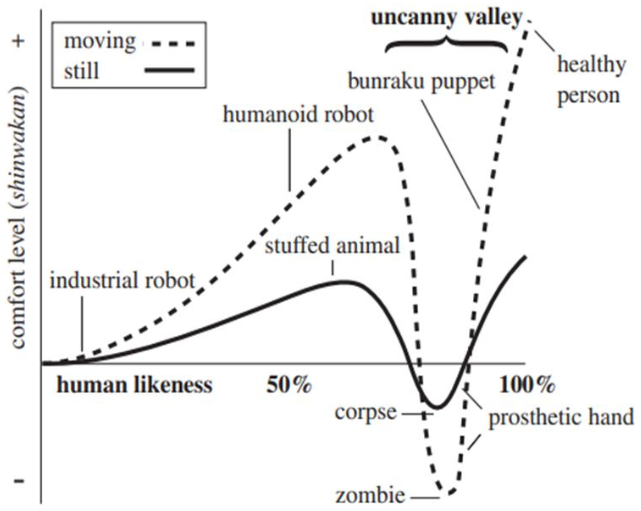
\includegraphics[width=\textwidth]{04-1_mori_1970_uncanny_valley_curve}\\[0.2em]
      {\tiny\color{kngrey}Mori 1970: comfort against human likeness~[1]\par}
    \end{column}
  \end{columns}
\end{frame}

%% ============================================================
%% CHAPTER 3 — RELATED WORK
%% ============================================================

\begin{frame}[plain]
  \vspace{2.4em}
  \begin{center}
    \colorbox{kncyan}{\parbox{0.52\textwidth}{\centering\vspace{7pt}\fontsize{24}{28}\selectfont\bfseries\color{black} Related Work\vspace{7pt}}}
  \end{center}
  \vfill
  \hbox{\color{knrule}\rule{\paperwidth}{0.9pt}}
  \vspace{0.6em}
\end{frame}

\begin{frame}{1. Measuring the Valley}{Chapter 3 — from a drawn curve, to data, to an instrument, to CG characters}
  \vspace{0.3em}
  \begin{columns}[c]
    \begin{column}{0.235\textwidth}\centering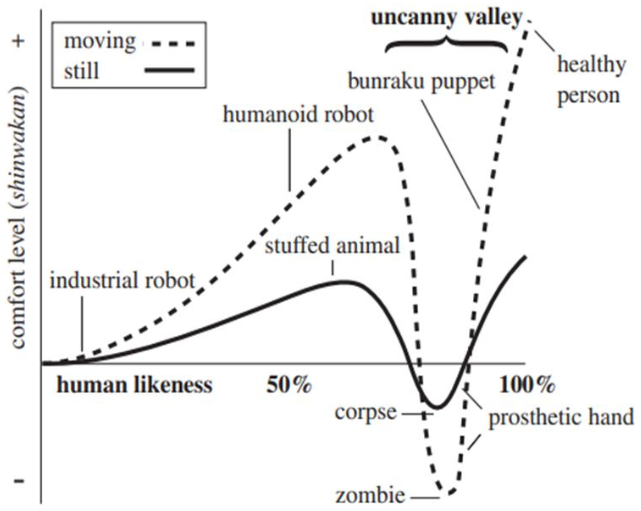
\includegraphics[height=1.75cm,width=0.95\textwidth,keepaspectratio]{04-1_mori_1970_uncanny_valley_curve}\end{column}
    \begin{column}{0.235\textwidth}\centering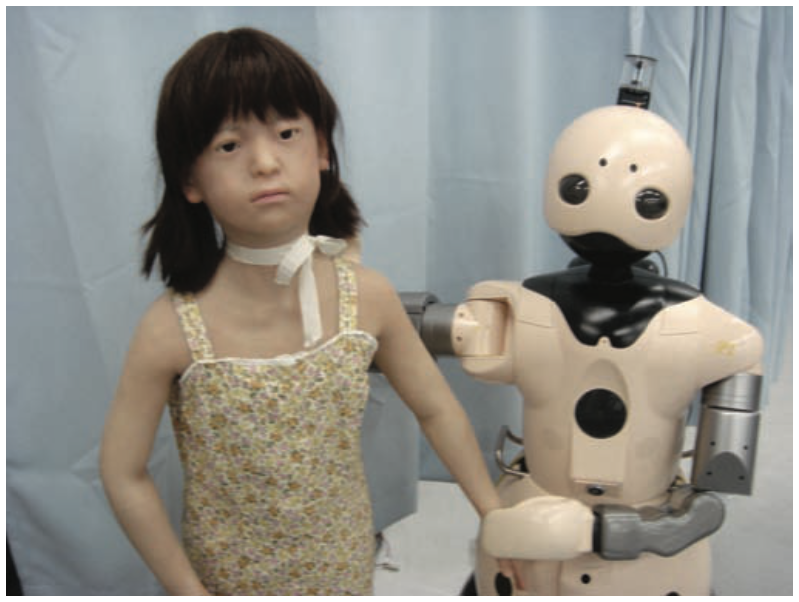
\includegraphics[height=1.75cm,width=0.95\textwidth,keepaspectratio]{04-2_macdorman_2006_android_and_robot}\end{column}
    \begin{column}{0.235\textwidth}\centering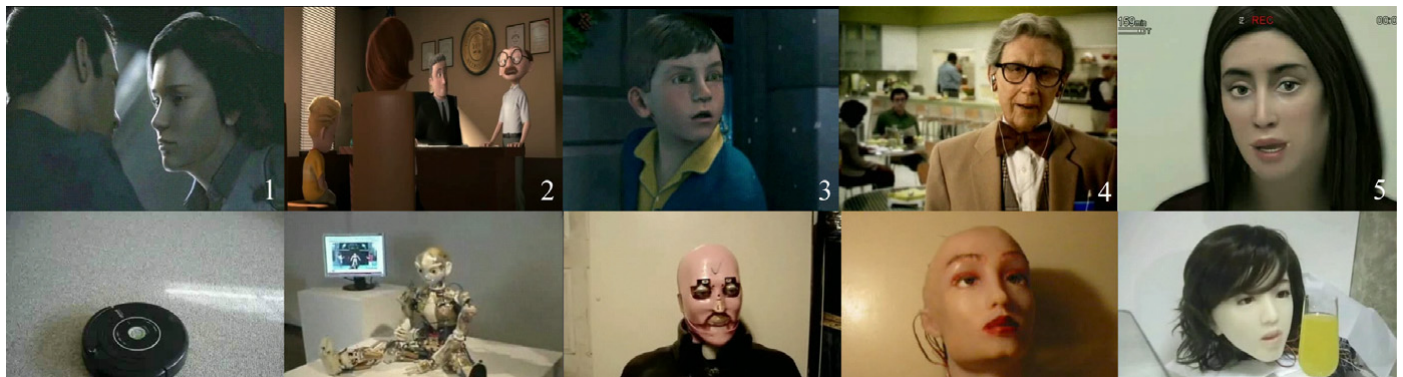
\includegraphics[height=1.75cm,width=0.95\textwidth,keepaspectratio]{04-3_ho_macdorman_2010_stimuli}\end{column}
    \begin{column}{0.235\textwidth}\centering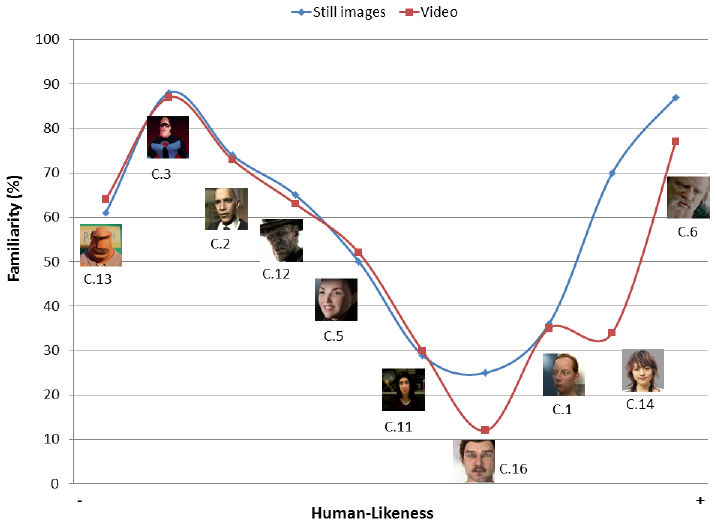
\includegraphics[height=1.75cm,width=0.95\textwidth,keepaspectratio]{04-4_dill_2012_cg_character_curve}\end{column}
  \end{columns}
  \vspace{0.35em}
  \begin{center}
  
\begin{tikzpicture}
    \draw[knrule, line width=1.1pt] (0,0) -- (0.93\textwidth,0);
    \foreach \i/\n in {0.115/01, 0.375/02, 0.635/03, 0.895/04}
      \node[circle, fill=kncyan, text=white, font=\tiny\bfseries, inner sep=2.2pt]
        at (\i*0.93\textwidth,0) {\n};
  \end{tikzpicture}
  \end{center}
  \vspace{0.15em}
  \begin{columns}[T]
    \begin{column}{0.235\textwidth}\centering
      {\scriptsize\bfseries 1970, Mori}\\[0.25em]
      {\tiny\color{knblue}\itshape The Uncanny Valley~[1]}\\[0.4em]
      {\scriptsize \hl{Proposed it.} Comfort drops just short of human, and \hl{motion deepens the dip}.}
    \end{column}
    \begin{column}{0.235\textwidth}\centering
      {\scriptsize\bfseries 2006, MacDorman \& Ishiguro}\\[0.25em]
      {\tiny\color{knblue}\itshape The Uncanny Advantage of Using Androids~[2]}\\[0.4em]
      {\scriptsize \hl{Measured it.} Eeriness peaks where \hl{comfort is lowest}.}
    \end{column}
    \begin{column}{0.235\textwidth}\centering
      {\scriptsize\bfseries 2010, Ho \& MacDorman}\\[0.25em]
      {\tiny\color{knblue}\itshape Revisiting the Uncanny Valley Theory~[3]}\\[0.4em]
      {\scriptsize \hl{Instrumented it.} Eeriness becomes \hl{separable from likeness}.}
    \end{column}
    \begin{column}{0.235\textwidth}\centering
      {\scriptsize\bfseries 2012, Dill et al.}\\[0.25em]
      {\tiny\color{knblue}\itshape Evaluation of the Uncanny Valley in CG Characters~[4]}\\[0.4em]
      {\scriptsize \hl{Extended it.} It appears for \hl{CG characters}, worst at the \hl{eyes and mouth}.}
    \end{column}
  \end{columns}
  \takeaway{The valley is real, measurable and reaches CG avatars. None of it says whether a viewer would \emph{rely} on one.}
\end{frame}

\begin{frame}{2. Trust and the Valley}{Chapter 3 — the valley reaches trust, and trust has three parts}
  \vspace{0.3em}
  \begin{columns}[T]
    \begin{column}{0.30\textwidth}\centering
      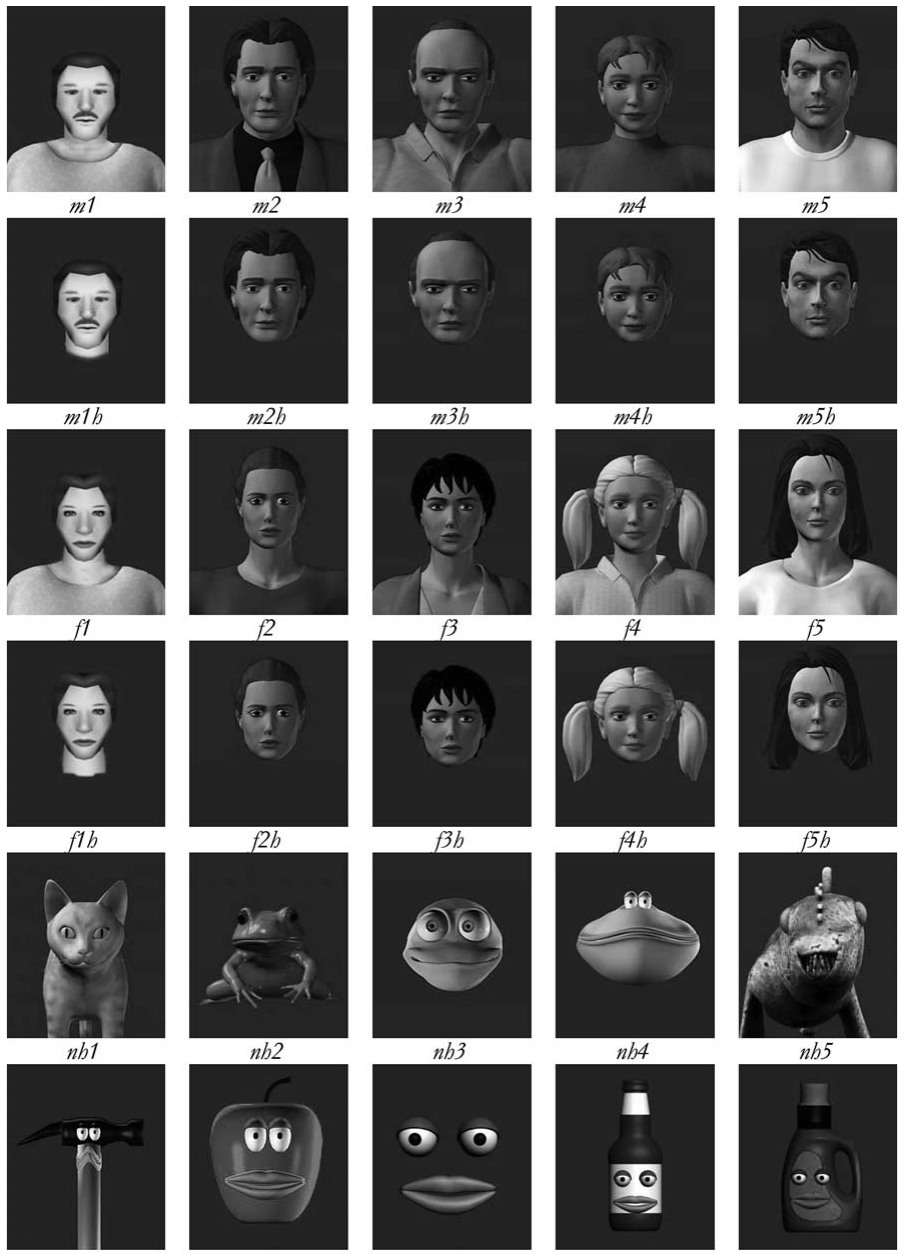
\includegraphics[height=2.0cm,width=0.92\textwidth,keepaspectratio]{05-1_nowak_rauh_2005_avatar_set}
      \vspace{0.35em}

      
\begin{tikzpicture}
        \draw[knrule, line width=1.1pt] (0,0) -- (0.26\textwidth,0);
        \node[circle, fill=kncyan, text=white, font=\tiny\bfseries, inner sep=2.2pt] at (0.13\textwidth,0) {01};
      \end{tikzpicture}
      \vspace{0.2em}

      {\scriptsize\bfseries 2005, Nowak \& Rauh}\\[0.2em]
      {\tiny\color{knblue}\itshape The Influence of the Avatar on Online Perceptions~[5]}\\[0.35em]
      {\scriptsize \hl{Tested credibility.} More human-like avatars rated \hl{more credible}.}
    \end{column}
    \begin{column}{0.66\textwidth}
      \panelheadsm{So How Is Trust Measured?}
      \noindent\colorbox{knlight}{\parbox{0.96\textwidth}{\vspace{2pt}\scriptsize
        \hl{Ability.} Can they actually do this? Competence inside one domain, not in general.\vspace{2pt}}}
      \vspace{0.3em}

      \noindent\colorbox{knlight}{\parbox{0.96\textwidth}{\vspace{2pt}\scriptsize
        \hl{Benevolence.} Are they on my side? The belief that the other party cares about my wellbeing.\vspace{2pt}}}
      \vspace{0.3em}

      \noindent\colorbox{knlight}{\parbox{0.96\textwidth}{\vspace{2pt}\scriptsize
        \hl{Integrity.} Do they play straight? Principles I accept, and saying what they mean.\vspace{2pt}}}
      \vspace{0.35em}

      {\scriptsize\color{knblue} Mayer et al.\ 1995: trustworthiness has three \emph{separable} dimensions, not one score~[6]. All three measured, once per advisor.\par}
    \end{column}
  \end{columns}
  \takeaway{The valley reaches trust, not only comfort. And trust is not one number, which is why nothing in this talk reports a single trust score.}
\end{frame}

\begin{frame}{3. Abstraction as the Exit}{Chapter 3 — three studies, one meta-analysis, and they do not agree}
  \vspace{0.25em}
  \begin{columns}[c]
    \begin{column}{0.235\textwidth}\centering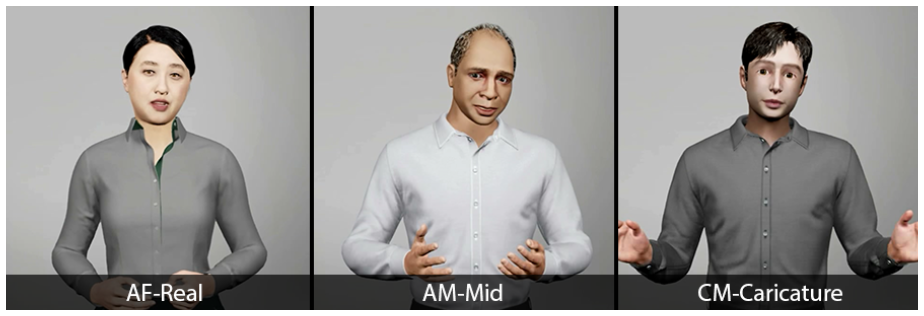
\includegraphics[height=1.9cm,width=0.95\textwidth,keepaspectratio]{06-2_canales_2024_stylisation_levels}\end{column}
    \begin{column}{0.235\textwidth}\centering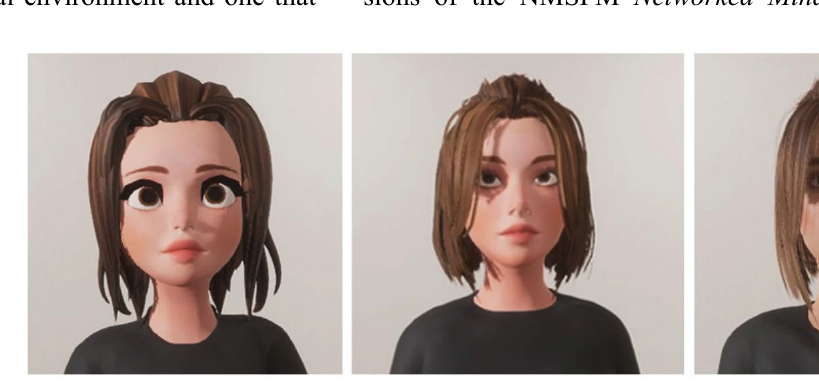
\includegraphics[height=1.9cm,width=0.95\textwidth,keepaspectratio]{06-4_dubosc_2025_stylisation_levels}\end{column}
    \begin{column}{0.235\textwidth}\centering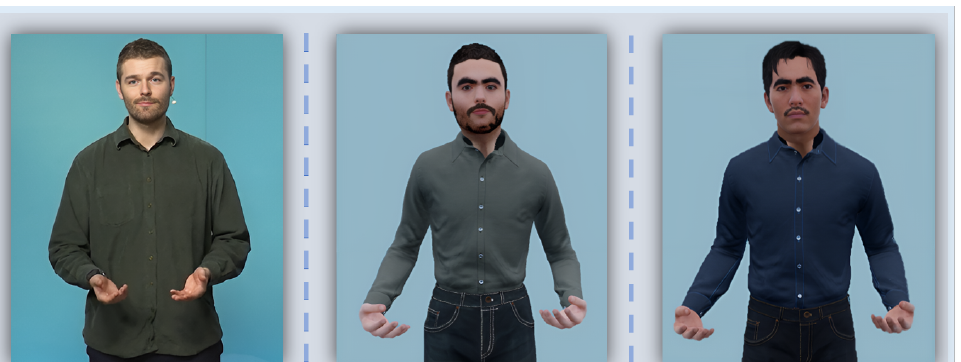
\includegraphics[height=1.9cm,width=0.95\textwidth,keepaspectratio]{06-3_gao_2025_real_vs_stylised}\end{column}
    \begin{column}{0.235\textwidth}\centering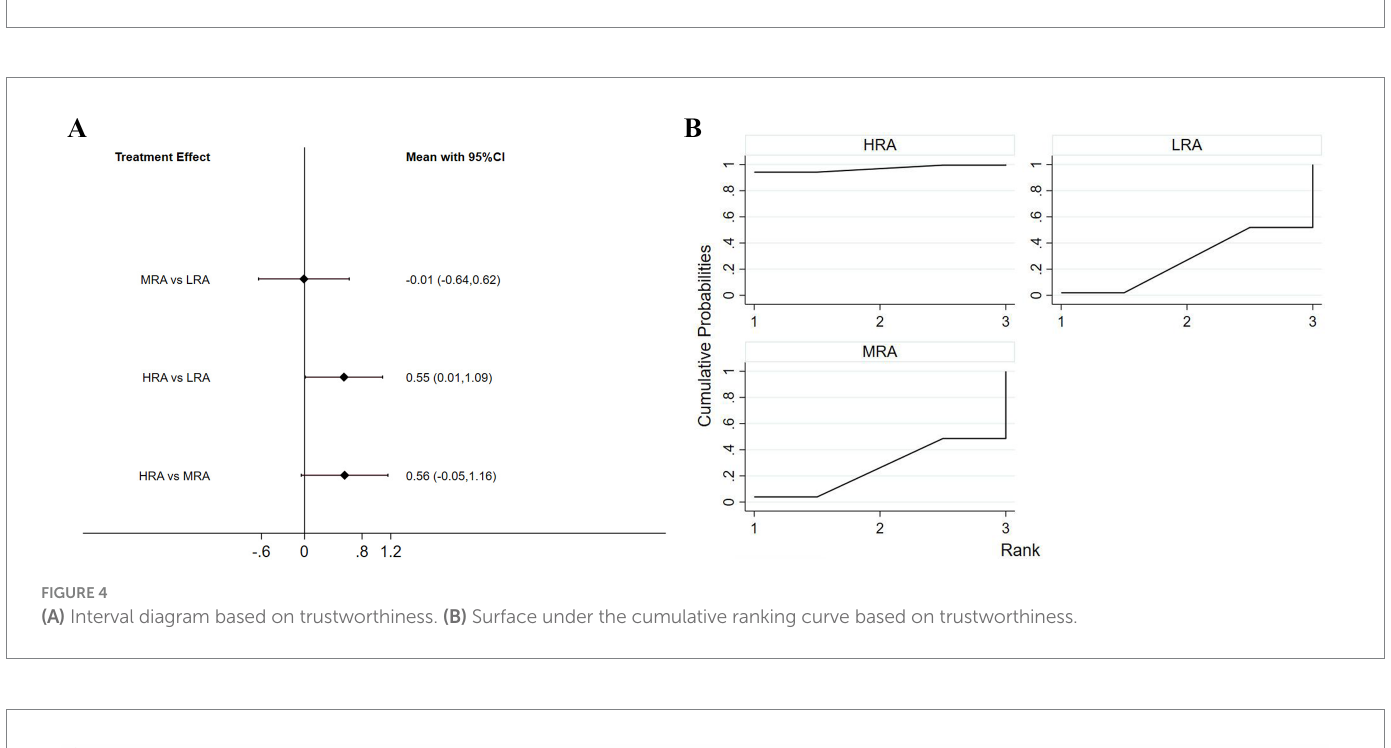
\includegraphics[height=1.9cm,width=0.95\textwidth,keepaspectratio]{06-5_tao_2025_trustworthiness_ranking}\end{column}
  \end{columns}
  \vspace{0.3em}
  \begin{center}
  
\begin{tikzpicture}
    \draw[knrule, line width=1.1pt] (0,0) -- (0.93\textwidth,0);
    \foreach \i/\n in {0.115/01, 0.375/02}
      \node[circle, fill=kngreen, text=white, font=\tiny\bfseries, inner sep=2.2pt]
        at (\i*0.93\textwidth,0) {\n};
    \foreach \i/\n in {0.635/03, 0.895/04}
      \node[circle, fill=knred, text=white, font=\tiny\bfseries, inner sep=2.2pt]
        at (\i*0.93\textwidth,0) {\n};
  \end{tikzpicture}
  \end{center}
  \vspace{0.15em}
  \begin{columns}[T]
    \begin{column}{0.235\textwidth}\centering
      {\scriptsize\bfseries 2024, Canales et al.}\\[0.2em]
      {\tiny\color{knblue}\itshape The Impact of Avatar Stylization on Trust~[7]}\\[0.3em]
      {\scriptsize \hl{Same Mayer model.} Three levels. Self-report \hl{flat}, but 48\% chose the \hl{semi-realistic} doctor.}
    \end{column}
    \begin{column}{0.235\textwidth}\centering
      {\scriptsize\bfseries 2025, Dubosc et al.}\\[0.2em]
      {\tiny\color{knblue}\itshape Effect of Avatar Stylization and Facial Expression Intensity~[8]}\\[0.3em]
      {\scriptsize Face to face in VR. Stylised avatars rated significantly \hl{less eerie}.}
    \end{column}
    \begin{column}{0.235\textwidth}\centering
      {\scriptsize\bfseries 2025, Gao et al.}\\[0.2em]
      {\tiny\color{knblue}\itshape Trust in Virtual Agents~[9]}\\[0.3em]
      {\scriptsize An agent against the real speaker. The \bad{real speaker} won on all three dimensions, but \hl{not on overall trust}.}
    \end{column}
    \begin{column}{0.235\textwidth}\centering
      {\scriptsize\bfseries 2025, Tao et al.}\\[0.2em]
      {\tiny\color{knblue}\itshape Impact of Virtual Avatar Appearance Realism~[10]}\\[0.3em]
      {\scriptsize \hl{Meta-analysis}, 13 studies. \bad{High realism} more trustworthy than low, but not than medium.}
    \end{column}
  \end{columns}
  \takeaway{Two say abstraction helps, two favour realism, and neither side is clean. The evidence has not converged, which is what RQ3 goes after.}
\end{frame}

\begin{frame}{Research Questions}{Chapter 1 — three gaps in the work just shown, three questions}
  \vspace{0.4em}
  \begin{columns}[T]
    \begin{column}{0.53\textwidth}
      \panelhead{Three Research Questions}
      \noindent\colorbox{knlight}{\parbox{0.96\textwidth}{\vspace{3pt}\scriptsize
        \textbf{RQ1} Technical transfer \hfill \hl{System}\\[0.15em]
        How can NPR techniques be adapted to platforms with different rendering architectures, and what capabilities and limitations does each impose?\\[0.5em]
        \textbf{RQ2} Technique selection \hfill \hl{Experiment 1}\\[0.15em]
        Which technique or combination best balances visual abstraction against facial and expressive legibility?\\[0.5em]
        \textbf{RQ3} Perception \hfill \hl{Experiment 2}\\[0.15em]
        How does stylisation affect eeriness and trustworthiness, and can it reach the trustworthiness of a photorealistic avatar and of a real human speaker?\vspace{3pt}}}
    \end{column}
    \begin{column}{0.45\textwidth}
      \panelhead{Four Contributions}
      \panel{%
        \item \hl{System:} eight NPR techniques, three production avatar platforms, runtime-selectable
        \item \hl{Calibration:} parameters set by preference testing, not by eye
        \item \hl{Design:} ratings and behavioural choice together, rendering style isolated from confounds
        \item \hl{Evidence:} trust against a photorealistic avatar \emph{and} a real human}
    \end{column}
  \end{columns}
\end{frame}

%% ============================================================
%% CHAPTER 4 — METHODOLOGY: THE SYSTEM
%% ============================================================

\begin{frame}[plain]
  \vspace{2.4em}
  \begin{center}
    \colorbox{kncyan}{\parbox{0.80\textwidth}{\centering\vspace{7pt}\fontsize{24}{28}\selectfont\bfseries\color{black} Methodology and Evaluation\vspace{7pt}}}
  \end{center}
  \vfill
  \hbox{\color{knrule}\rule{\paperwidth}{0.9pt}}
  \vspace{0.6em}
\end{frame}

\begin{frame}{Three Avatar Platforms}{Chapter 4.2 — chosen to span the range of pipeline access}
  \vspace{0.3em}
  \begin{columns}[T]
    \begin{column}{0.63\textwidth}
      \scriptsize
      \setlength{\tabcolsep}{4pt}\renewcommand{\arraystretch}{1.45}
      \begin{tabular}{@{}>{\raggedright\arraybackslash}m{0.21\textwidth}>{\raggedright\arraybackslash}m{0.24\textwidth}>{\raggedright\arraybackslash}m{0.26\textwidth}>{\raggedright\arraybackslash}m{0.24\textwidth}@{}}
        \toprule
        & \textbf{Mixamo} & \textbf{Meta SDK} & \textbf{Avaturn} \\
        \midrule
        Shader access    & \good{Full URP}, unrestricted & \bad{Hook injection only}, after SDK lighting & \good{Full URP}, unrestricted \\
        \rowrule
        Facial animation & \bad{None} & Requires \hl{Quest~Pro} hardware & \good{Blendshape animation} \\
        \rowrule
        Key challenge    & No facial rigging & Shader manipulation & Initial Unity import \\
        \rowrule
        Strength         & Full shader freedom~[11] & Native Quest~3 integration~[12] & \hl{High fidelity facial quality}~[13] \\
        \bottomrule
      \end{tabular}
    \end{column}
    \begin{column}{0.34\textwidth}
      \panelhead{Why Avaturn for the Study}
      \panel{%
        \item The only one with a \hl{realistic face} that can also be \hl{animated}
        \item The study avatar was built from photographs of the real speaker
        \item All three were used to develop the eight techniques}
    \end{column}
  \end{columns}
\end{frame}

\begin{frame}{Eight NPR Techniques}{Chapters 4 and 6.1 — built iteratively, then assessed against four criteria}
  \vspace{0.25em}
  {\centering\tiny
  \setlength{\tabcolsep}{3pt}\renewcommand{\arraystretch}{1.28}
  \begin{tabular}{@{}>{\raggedright\arraybackslash}m{0.19\textwidth}>{\raggedright\arraybackslash}m{0.145\textwidth}>{\raggedright\arraybackslash}m{0.125\textwidth}>{\raggedright\arraybackslash}m{0.11\textwidth}>{\raggedright\arraybackslash}m{0.125\textwidth}>{\raggedright\arraybackslash}m{0.125\textwidth}>{\raggedright\arraybackslash}m{0.08\textwidth}@{}}
    \toprule
    \textbf{Technique} & \textbf{What it adds} & \textbf{Facial readability} & \textbf{Temporal stability} & \textbf{Artefact suppression} & \textbf{Expressive abstraction} & \textbf{Candidate} \\
    \midrule
    V1 Geometric Silhouette Outline & Silhouette from geometry & \good{\checkmark} & \good{\checkmark} & (\checkmark) alpha cutout & \bad{$\times$} not in isolation & \good{\checkmark} \\
    \rowrule
    V2 Toon Shading & Quantised diffuse bands & \good{\checkmark} & \good{\checkmark} & \good{\checkmark} & (\checkmark) no interior lines & --- \\
    \rowrule
    V2.2 X-Toon Shading & 2D ramp: lighting \emph{and} abstraction & \good{\checkmark} & \good{\checkmark} & \good{\checkmark} & (\checkmark) manual mode & \good{\checkmark} \\
    \rowrule
    V3 Screen-Space Normal Edge Detection & Creases from normal derivatives & \bad{$\times$} landmarks missed & \good{\checkmark} & \good{\checkmark} & \good{\checkmark} & --- \\
    \rowrule
    V4 Sobel Edge Detection & Colour-buffer gradients & (\checkmark) threshold & (\checkmark) & (\checkmark) preprocessing & \good{\checkmark} & \good{\checkmark} \\
    \rowrule
    V4.2 Gaussian Prefiltered Sobel & Smoothing before differentiation & \bad{$\times$} no gain over V4 & (\checkmark) & \good{\checkmark} & \good{\checkmark} & --- \\
    \rowrule
    V5 Hierarchical Edge Detection with Multiple Cues & Depth, normal and colour merged & \bad{$\times$} segments unclear & \good{\checkmark} & \bad{$\times$} nose bridge & \good{\checkmark} & \good{\checkmark} \\
    \rowrule
    V6 Kuwahara Painterly Filter & Painterly surface abstraction & \bad{$\times$} at large radius & \good{\checkmark} & \good{\checkmark} & \good{\checkmark} & \good{\checkmark} \\
    \bottomrule
  \end{tabular}\par}
  \vspace{0.2em}
  {\centering\tiny\color{kngrey}{\color{kngreen}\checkmark} satisfactory without tuning \quad {\color{kngrey}(\checkmark)} satisfactory after tuning \quad {\color{knred}$\times$} limitation observed\par}
  \vfill
  \noindent\colorbox{knlight}{\parbox{0.975\textwidth}{\scriptsize\color{knblue}
  Each technique was built to resolve a limitation of the one before. \textbf{No technique satisfied all four criteria alone}, and \textbf{facial readability} failed most often, four times out of eight. \textbf{Five went forward} as candidates for the composite.}}
\end{frame}

\begin{frame}{Applying the Techniques}{Chapter 4 — the texture based detectors failed on the study avatar}
  \vspace{0.3em}
  \begin{columns}[T]
    \begin{column}{0.62\textwidth}
      \centering
      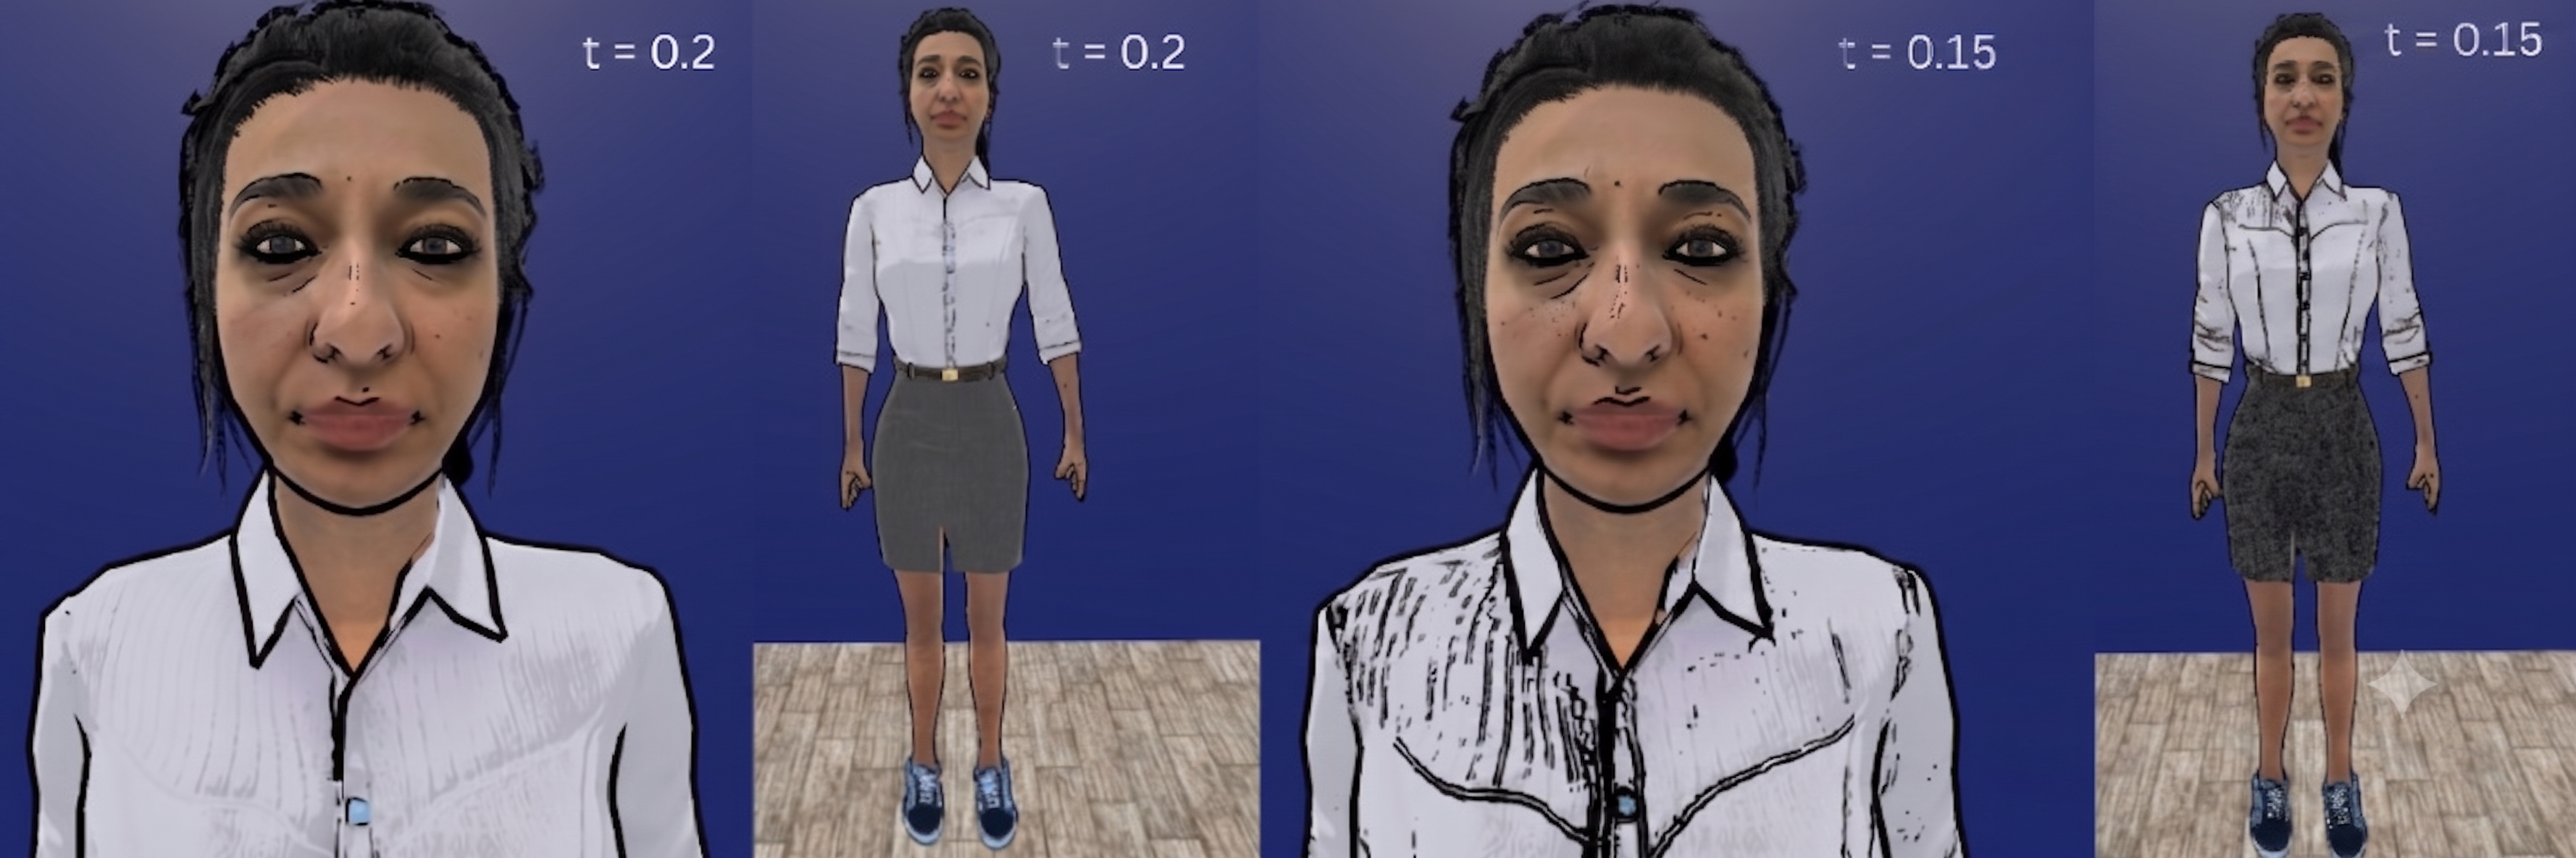
\includegraphics[width=0.80\textwidth]{technique_V4-2_gaussian_sobel_avaturn}\\[0.2em]
      {\scriptsize\color{knblue}\textbf{V4.2} Gaussian Prefiltered Sobel}
      \vspace{0.35em}

      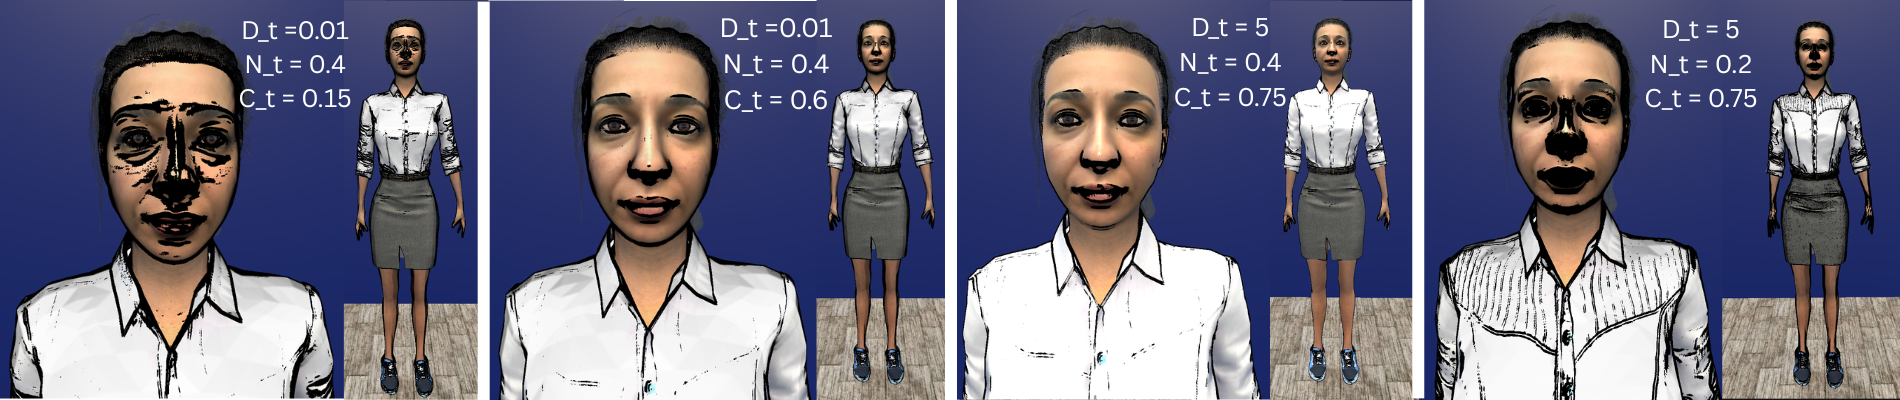
\includegraphics[width=0.80\textwidth]{technique_V5_hierarchical_sweep_avaturn}\\[0.2em]
      {\scriptsize\color{knblue}\textbf{V5} Hierarchical Edge Detection with Multiple Cues}
    \end{column}
    \begin{column}{0.35\textwidth}
      \panelhead{What the Detectors Produced}
      \panel{%
        \item Lines where there is no feature
        \item \hl{Eyebrows and lip line barely register}
        \item V4.2: smoother, features still missing
        \item V5: brow and nose shadow become hard edges}
      \vspace{0.4em}
      \panelhead{Why}
      \panel{%
        \item Head rebuilt from \hl{photographs}
        \item \hl{Baked illumination} and \hl{fine skin noise} both read as structure
        \item Smoothing removes the noise \emph{and} the real edges together
        \item No threshold separates them}
    \end{column}
  \end{columns}
\end{frame}

\begin{frame}{Avatar Texture Manipulation}{Chapter 4 — fixing the input instead of the operator}
  \vspace{0.25em}
  \begin{columns}[T]
    \begin{column}{0.36\textwidth}
      \panelhead{Three Edits in Blender}
      \panel{%
        \item Baked illumination blurred out
        \item Skin tone unified
        \item Mouth saturation raised, lip line added}
      \vspace{0.15em}
      \panelhead{What It Recovered}
      \panel{%
        \item \hl{Lip line and eyebrows} now detectable
        \item Gaussian prefilter no longer needed}
      \vspace{0.15em}
      \panelhead{Scope}
      \panel{%
        \item Applied to the \hl{NPR avatar} only
        \item Photorealistic version keeps original texture}
    \end{column}
    \begin{column}{0.61\textwidth}
      \centering
      \vspace{0.6em}
      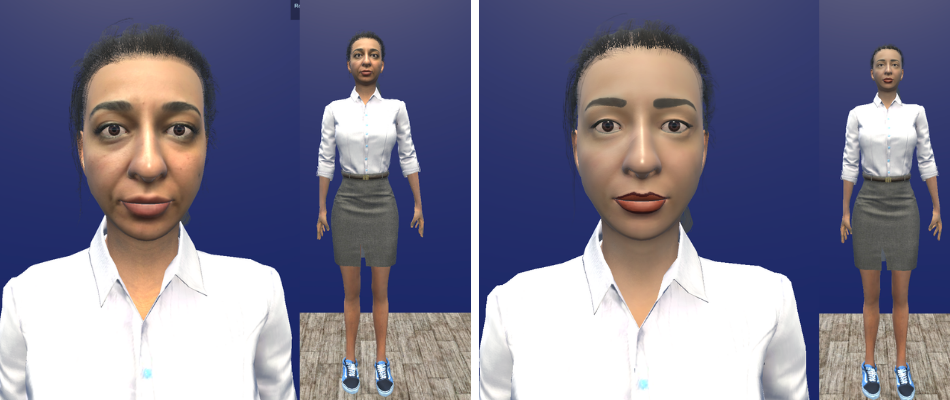
\includegraphics[width=\textwidth]{texture_0_default_vs_preprocessed}\\[0.45em]
      \makebox[0.48\textwidth]{\scriptsize\color{kngrey}Default Avaturn}\hfill
      \makebox[0.48\textwidth]{\scriptsize\color{kngrey}Preprocessed head texture}
    \end{column}
  \end{columns}
\end{frame}


%% ============================================================
%% EXPERIMENT 1 — PARAMETER ADJUSTMENT STUDY
%% ============================================================

\begin{frame}[plain]
  \vspace{2.4em}
  \begin{center}
    \colorbox{kncyan}{\parbox{0.72\textwidth}{\centering\vspace{7pt}\fontsize{24}{28}\selectfont\bfseries\color{black} Experiment 1 — Parameter Adjustment Study\vspace{7pt}}}
  \end{center}
  \vfill
  \hbox{\color{knrule}\rule{\paperwidth}{0.9pt}}
  \vspace{0.6em}
\end{frame}

\begin{frame}{Parameter Adjustment Study — Design}{Chapter 4.8 — calibration by preference, not by inspection}
  \vspace{0.3em}
  {\scriptsize
  \begin{itemize}\setlength{\itemsep}{0.2em}
    \item \hl{45 participants} ranked rendered variants of the avatar by \hl{perceived trustworthiness}
    \item One parameter group per round, five rounds, and each round's outcome frozen for every round after it
    \item A closing question asked for the \hl{overall most visually appealing} avatar across all rounds
  \end{itemize}}
  \vspace{0.3em}
  {\centering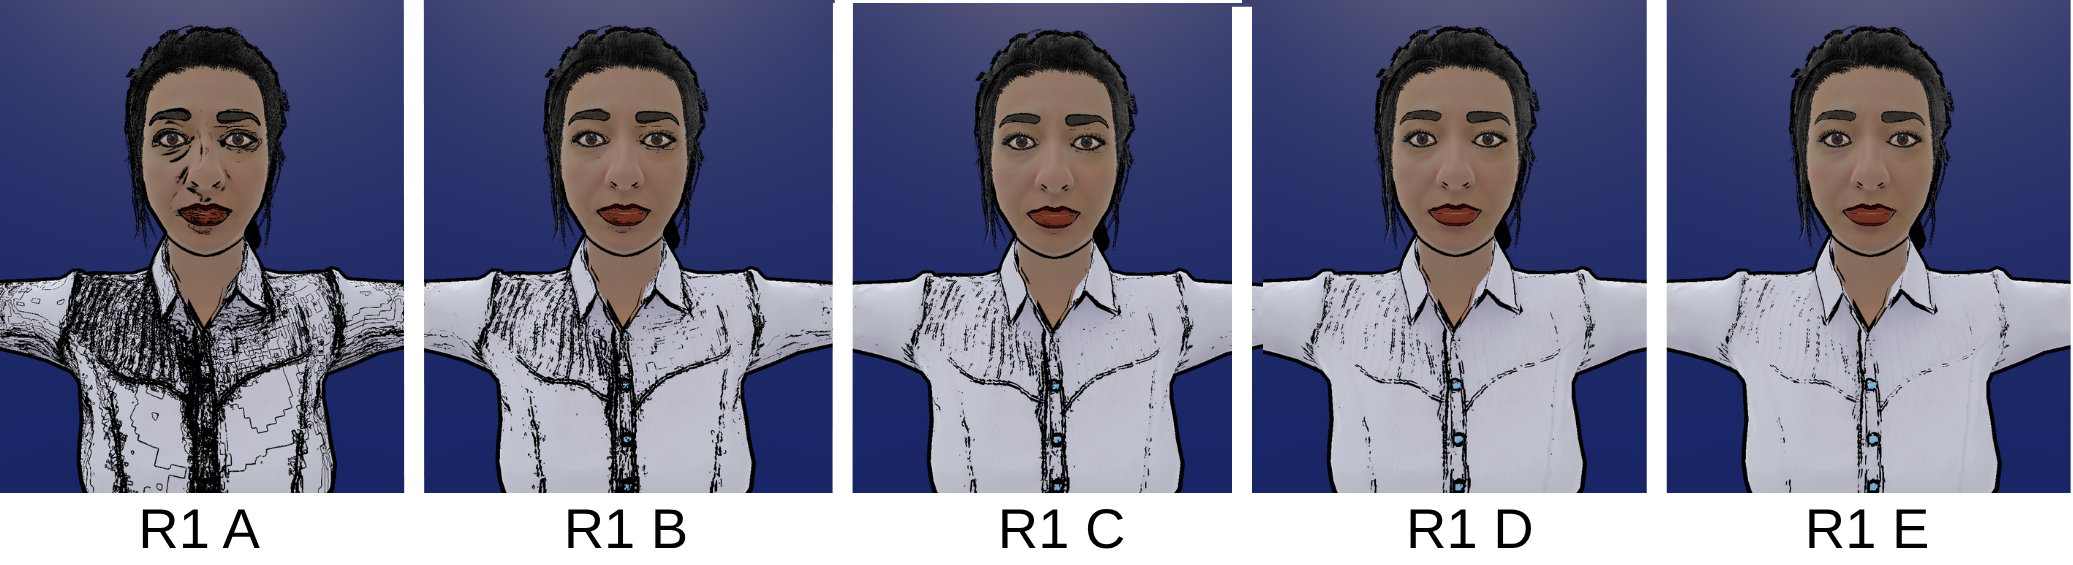
\includegraphics[width=0.66\textwidth]{prestudy_R1_threshold_sweep}\par}
  \vspace{0.05em}
  {\centering\tiny\color{kngrey} One round as an example. R1 inner line threshold, 0.01 to 0.05.\par}
  \vspace{0.3em}
  {\centering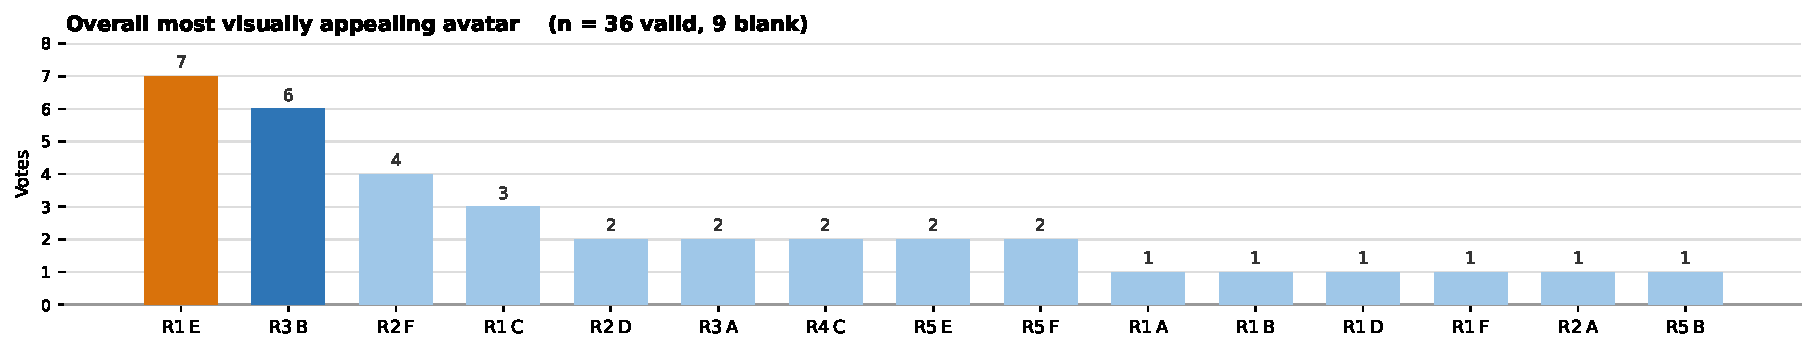
\includegraphics[width=0.74\textwidth]{prestudy_overall_appeal_wide}\par}
\end{frame}

\begin{frame}{Parameter Adjustment Study — Outcome}{Chapter 6.2.1 — what each round settled}
  \vspace{0.35em}
  \begin{columns}[T]
    \begin{column}{0.575\textwidth}
      \vspace{0.9em}
      \tiny
      \setlength{\tabcolsep}{4pt}\renewcommand{\arraystretch}{1.9}
      \begin{tabular}{@{}>{\raggedright\arraybackslash}m{0.05\textwidth}>{\raggedright\arraybackslash}m{0.325\textwidth}>{\raggedright\arraybackslash}m{0.15\textwidth}>{\raggedright\arraybackslash}m{0.185\textwidth}>{\raggedright\arraybackslash}m{0.235\textwidth}@{}}
        \toprule
        & \textbf{Parameter group} & \textbf{Winner} & \textbf{Significant?} & \textbf{Set to} \\
        \midrule
        R1 & Inner line threshold          & 0.03       & no, $p = .31$          & \hl{0.05} appeal \\
        \rowrule
        R2 & Outline width, depth offset   & 0.003, on  & no, $p = .82$          & \textbf{0.003, on} Borda \\
        \rowrule
        R3 & Shadow strength, detail bias  & 0.5 / 1.0  & no, $p = .53$          & \hl{0.0 / 0.5} appeal \\
        \rowrule
        R4 & Kuwahara hardness, sharpness  & \bad{none} & \good{yes, $p = .003$} & \bad{off} baseline won \\
        \rowrule
        R5 & Hierarchical depth threshold  & \bad{none} & \good{yes, $p < .001$} & \bad{off} baseline won \\
        \bottomrule
      \end{tabular}
    \end{column}
    \begin{column}{0.40\textwidth}
      \centering
      \vspace{-0.3em}
      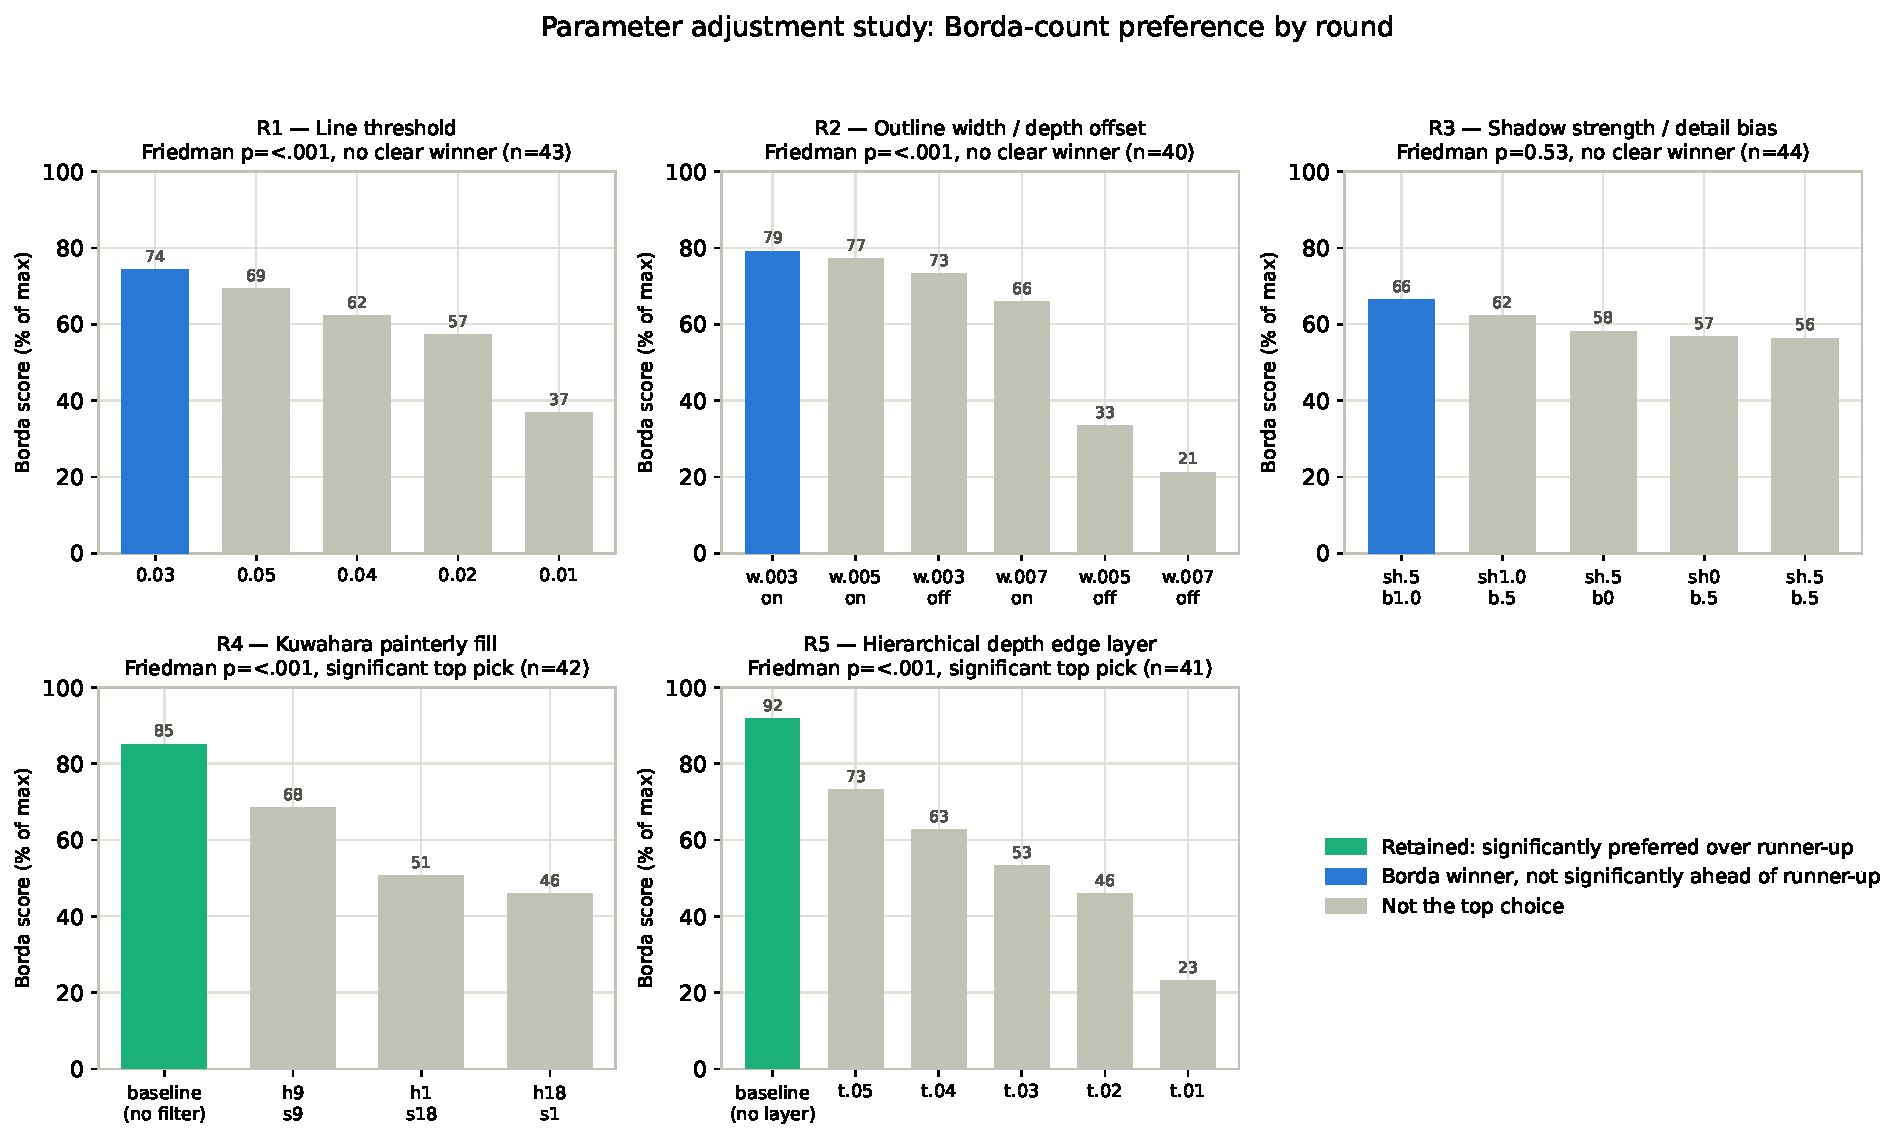
\includegraphics[height=0.36\textheight,width=\textwidth,keepaspectratio]{prestudy_summary}

      {\tiny\color{kngrey} Borda score per round. \textcolor{kngreen}{Green} = significantly preferred, \textcolor{knblue}{blue} = top choice, not clearly ahead.\par}
      \vspace{0.9em}

      \scriptsize
      \begin{itemize}\setlength{\itemsep}{0.2em}
        \item Ranks are \hl{ordinal}, so the tests are non-parametric
        \item \hl{Borda} scores the whole ballot, \hl{Friedman} tests the round against chance, \hl{Wilcoxon} compares the top two
        \item \bad{Kuwahara} and the \bad{hierarchical layer} dropped
        \item Composite: \hl{outline, X-Toon, Sobel}
      \end{itemize}
    \end{column}
  \end{columns}
\end{frame}

\begin{frame}{RQ1 and RQ2 Answers}{Chapters 4 and 6 — what the system work established}
  \vspace{0.4em}
  \begin{columns}[T]
    \begin{column}{0.49\textwidth}
      \panelhead{RQ1 \ Adaptation across Architectures}
      \panel{%
        \item All eight techniques ran on \hl{all three platforms}
        \item Same values, visibly different output per host: \hl{retuning always required}
        \item \bad{Meta SDK}: one fragment hook, no second pass, no depth buffer
        \item V5's depth cue became a \hl{camera-distance derivative}; V6's structure tensor lost its \hl{smoothing pass}}
    \end{column}
    \begin{column}{0.49\textwidth}
      \panelhead{RQ2 \ Abstraction versus Legibility}
      \panel{%
        \item On the raw texture, \bad{texture-based edge detection failed}
        \item After preprocessing, Sobel finds the \hl{eyebrows and lip line}; V4.2 no longer repays its 72 samples
        \item \good{Five of the eight} went forward as candidates
        \item The parameter study excluded \bad{V5} and \bad{V6}
        \item The answer is a \hl{composite}: V1 Geometric Silhouette Outline, V2.2 X-Toon Shading and V4 Sobel Edge Detection, over a preprocessed head texture}
    \end{column}
  \end{columns}
\end{frame}

%% ============================================================
%% EXPERIMENT 2 — MAIN USER STUDY
%% ============================================================

\begin{frame}[plain]
  \vspace{2.4em}
  \begin{center}
    \colorbox{kncyan}{\parbox{0.66\textwidth}{\centering\vspace{7pt}\fontsize{24}{28}\selectfont\bfseries\color{black} Experiment 2 — Main User Study\vspace{7pt}}}
  \end{center}
  \vfill
  \hbox{\color{knrule}\rule{\paperwidth}{0.9pt}}
  \vspace{0.6em}
\end{frame}

\begin{frame}{Main User Study — Design}{Chapter 4.10 — within-subjects, video based, three conditions}
  \vspace{-0.4em}
  \begin{columns}[T]
    \begin{column}{0.455\textwidth}
      \panelhead{Design}
      \panel{%
        \item 3 conditions $\times$ 3 scenarios (career, travel, learning)
        \item Three \hl{everyday domains}, avoiding carryover
        \item Recommended option alternates \hl{A, B, A}
        \item Paradigm after Canales et al.\ 2024~[7]}
      \vspace{0.1em}
      \panelheadsm{Order — $3\times3$ Latin Square, each condition once per slot}
      {\centering\tiny
      \setlength{\tabcolsep}{3pt}\renewcommand{\arraystretch}{1.12}
      \begin{tabular}{@{}lccc@{}}
        \toprule
        \textbf{Version} & \textbf{Video 1 Career} & \textbf{Video 2 Travel} & \textbf{Video 3 Learning} \\
        \midrule
        A & C2 & C1 & \hl{C3} \\
        B & \hl{C3} & C2 & C1 \\
        C & C1 & \hl{C3} & C2 \\
        \bottomrule
      \end{tabular}\par}
      \vspace{0.1em}
      \panelheadsm{Why Video Rather than VR}
      \noindent\colorbox{knlight}{\parbox{0.96\textwidth}{\vspace{2pt}\tiny
      \begin{itemize}\setlength{\itemsep}{0.15em}\setlength{\leftmargini}{0.9em}\setlength{\topsep}{0pt}\setlength{\parskip}{0pt}
        \item C1 has \bad{no VR equivalent}
        \item Video fixes \hl{one recorded performance}: the C2/C3 blendshape stream was captured while C1 was filmed
      \end{itemize}\vspace{2pt}}}
    \end{column}
    \begin{column}{0.525\textwidth}
      \begin{columns}[T]
        \begin{column}{0.315\textwidth}\centering
          \panelheadsm{C1 — Real}
          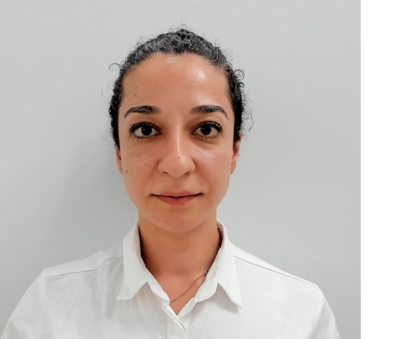
\includegraphics[height=2.35cm,width=\textwidth,keepaspectratio]{stimulus_C1_real}
        \end{column}
        \begin{column}{0.315\textwidth}\centering
          \panelheadsm{C2 — Photorealistic}
          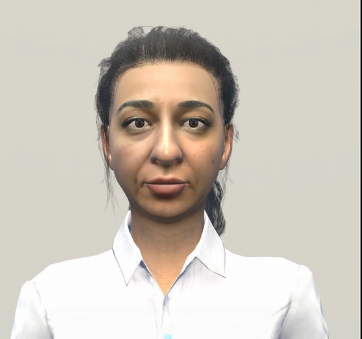
\includegraphics[height=2.35cm,width=\textwidth,keepaspectratio]{stimulus_C2_photorealistic}
        \end{column}
        \begin{column}{0.315\textwidth}\centering
          \panelheadsm{C3 — NPR}
          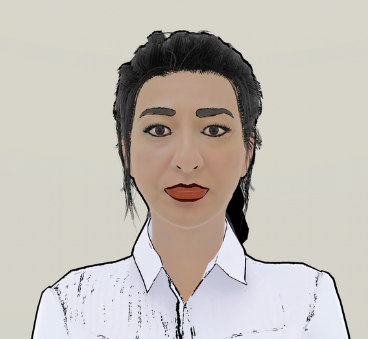
\includegraphics[height=2.35cm,width=\textwidth,keepaspectratio]{stimulus_C3_npr}
        \end{column}
      \end{columns}
      \vspace{0.2em}

      {\centering\tiny\color{kngrey}Same person, same animation, same voice. \textbf{C2 vs C3} is the critical pair.\par}
      \vspace{0.7em}

      \panelhead{Study Procedure}
      \centering
      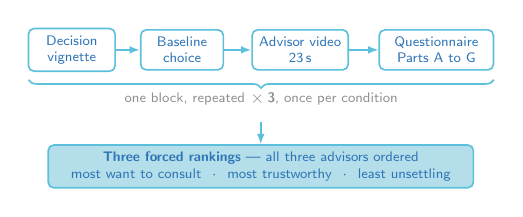
\begin{tikzpicture}[x=1cm, y=1cm,
          stepbox/.style={draw=knrule, line width=0.6pt, fill=white, rounded corners=2pt,
                          align=center, font=\tiny, text=knblue, inner sep=2.5pt, minimum height=0.48cm},
          arr/.style={-{Latex[length=1.3mm]}, knrule, line width=0.6pt},
          lbl/.style={font=\tiny, text=kngrey}]
        \node[stepbox, minimum width=1.10cm] (s1) at (0.72,0) {Decision\\vignette};
        \node[stepbox, minimum width=1.05cm] (s2) at (2.12,0) {Baseline\\choice};
        \node[stepbox, minimum width=1.22cm] (s3) at (3.62,0) {Advisor video\\23\,s};
        \node[stepbox, minimum width=1.45cm] (s4) at (5.35,0) {Questionnaire\\Parts A to G};
        \foreach \a/\b in {s1/s2, s2/s3, s3/s4} \draw[arr] (\a) -- (\b);
        \draw[decorate, decoration={brace, amplitude=3pt, mirror}, knrule, line width=0.6pt]
          (0.17,-0.38) -- (6.08,-0.38)
          node[midway, below=1pt, lbl] {one block, repeated \textbf{$\times$\,3}, once per condition};
        \node[stepbox, fill=knpale, minimum width=5.4cm] (r) at (3.12,-1.48)
          {\textbf{Three forced rankings} --- all three advisors ordered\\
           most want to consult \ $\cdot$ \ most trustworthy \ $\cdot$ \ least unsettling};
        \draw[arr] (3.12,-0.92) -- (r);
      \end{tikzpicture}
    \end{column}
  \end{columns}
\end{frame}

\begin{frame}{Hypotheses and the Subscales}{Chapter 4.10.1 — what was predicted, and what the ratings did}
  \vspace{0.3em}
  \begin{columns}[T]
    \begin{column}{0.40\textwidth}
      \panelhead{4 Hypotheses \& Statistical Tests}
      \noindent\colorbox{knlight}{\parbox{0.96\textwidth}{\vspace{3pt}\scriptsize
      \textbf{H1} \ NPR (C3) is rated \emph{less eerie} than the photorealistic avatar (C2).\newline
      {\color{knblue}\textbf{Test:}} RM-ANOVA, Holm pairwise\\[0.5em]
      \textbf{H2} \ NPR (C3) does \emph{not} cost trust relative to C2.\newline
      {\color{knblue}\textbf{Test:}} Pairwise plus TOST equivalence, $d = 0.3$ bound\\[0.5em]
      \textbf{H3} \ Eeriness lowers trust, likeability raises it, within participant.\newline
      {\color{knblue}\textbf{Test:}} Person-centred multilevel regression\\[0.5em]
      \textbf{H4} \ NPR (C3) does \emph{not} cost trust relative to the real speaker (C1).\newline
      {\color{knblue}\textbf{Test:}} Same as H2, against C1\vspace{3pt}}}
      \vspace{0.5em}

      {\scriptsize\color{knblue} H2 and H4 predict a \textbf{null}. A non-significant $p$ is not equivalence, hence the \textbf{TOST} bound, fixed in advance.\par}
    \end{column}
    \begin{column}{0.575\textwidth}
      \centering
      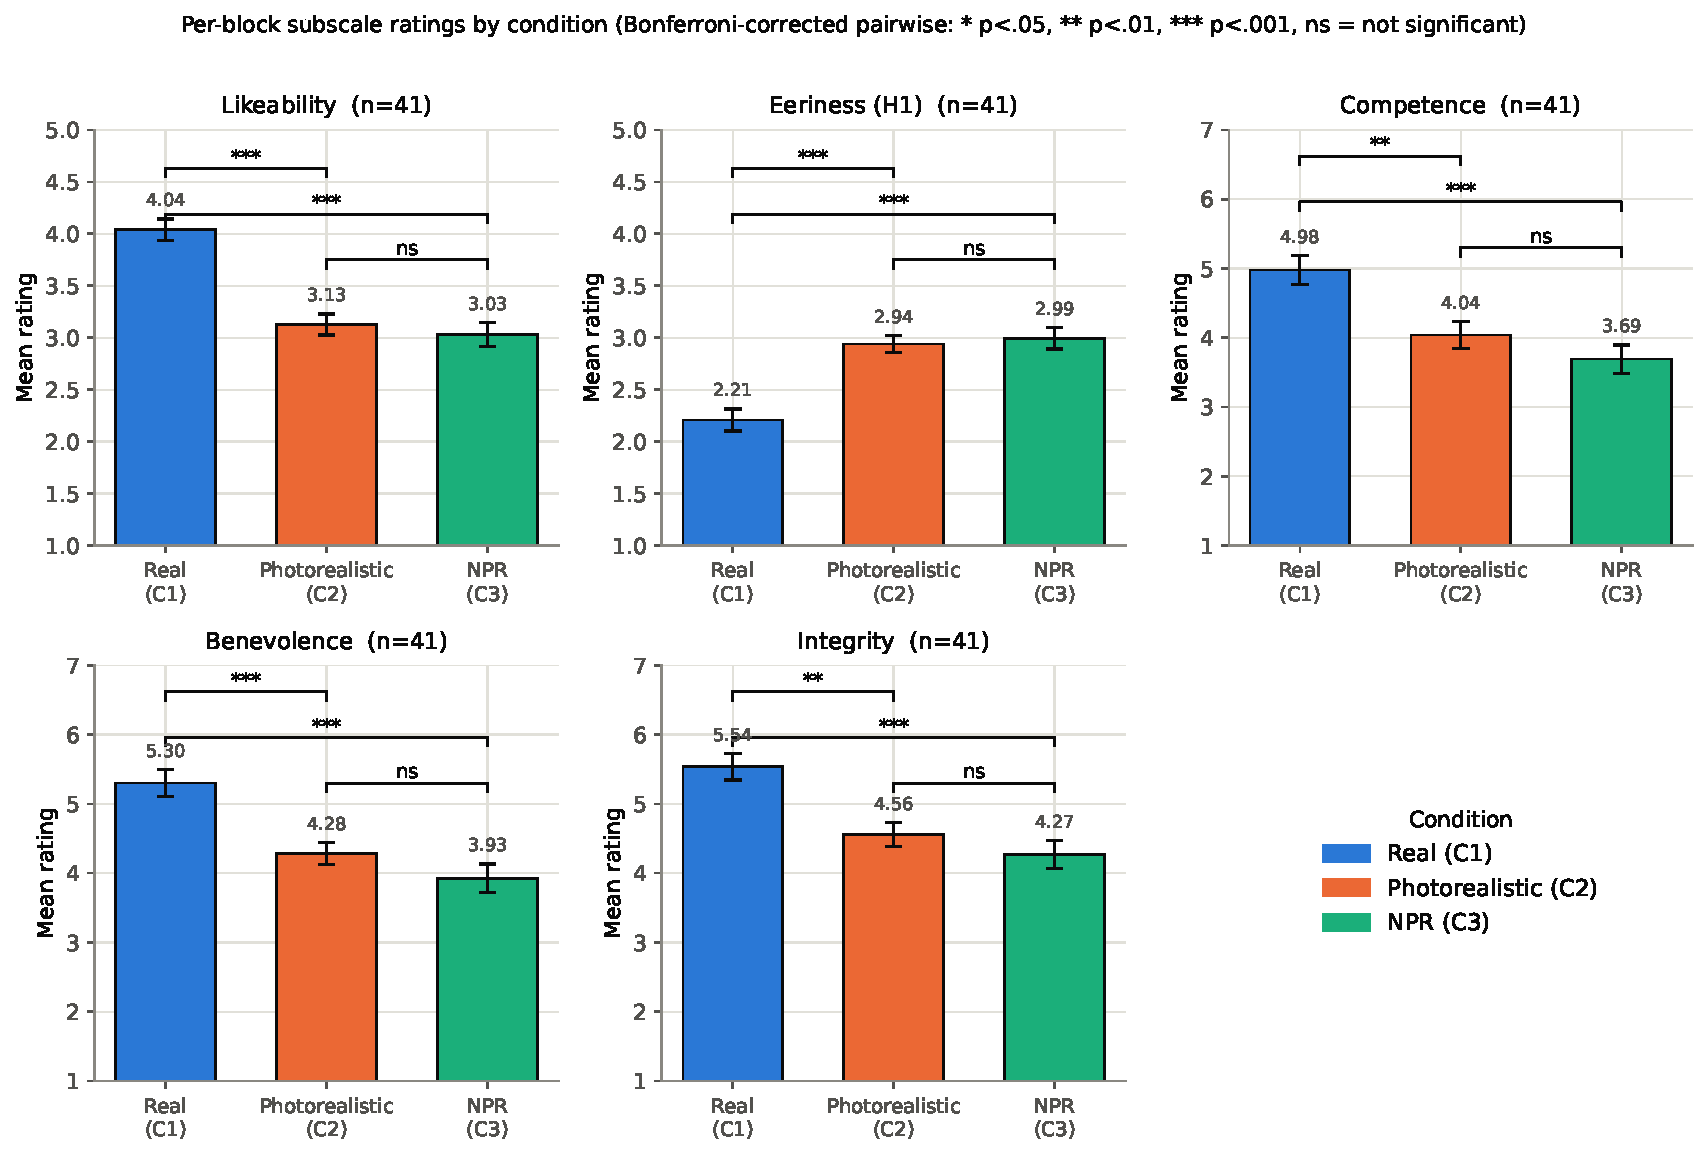
\includegraphics[width=\textwidth]{fig_subscales_grid}\\[0.3em]
      {\scriptsize\color{knblue}\textbf{The real speaker separates from both avatars on every subscale. The two avatars separate from each other on \emph{none} of them.}\par}
    \end{column}
  \end{columns}
\end{frame}

\begin{frame}{Measures and Analysis Plan}{Chapter 4.10.4 and 6.2.4 — validated instruments, the power carried, and did they see the difference?}
  \vspace{0.3em}
  \begin{columns}[T]
    \begin{column}{0.325\textwidth}
      \panelheadsm{Per-Block Questionnaire}
      \noindent\colorbox{knlight}{\parbox{0.96\textwidth}{\vspace{2pt}\tiny
      \setlength{\tabcolsep}{3pt}\renewcommand{\arraystretch}{1.28}
      \begin{tabular}{@{}>{\raggedright\arraybackslash}m{0.05\textwidth}>{\raggedright\arraybackslash}m{0.34\textwidth}>{\raggedright\arraybackslash}m{0.53\textwidth}@{}}
        A & Comprehension, gating & \bad{exclusion rule} \\
        B & Likeability, 5 items & Godspeed, Bartneck et al.\ 2009~[14] \\
        C & Eeriness, 8 items & Ho \& MacDorman 2010~[3] \\
        D & Ability, 3 items & Mayer et al.\ 1995~[6], wording adapted from Canales et al.\ 2024~[7] \\
        E & Benevolence, 3 items & Mayer et al.\ 1995~[6], wording adapted from Canales et al.\ 2024~[7] \\
        F & Integrity, 3 items & Mayer et al.\ 1995~[6], wording adapted from Canales et al.\ 2024~[7] \\
        G & Recommendation agreement & secondary \\
      \end{tabular}\vspace{2pt}}}
      \vspace{0.2em}
      {\tiny\color{kngrey}B and C on a 5-point semantic differential, D to G on a 7-point Likert.\par}
      \vspace{0.15em}
      {\tiny\color{kngrey}Composite reliability $\alpha=.87$ to $.96$.\par}
    \end{column}
    \begin{column}{0.275\textwidth}
      \panelheadsm{Analysis Plan}
      \noindent\colorbox{knlight}{\parbox{0.96\textwidth}{\vspace{2pt}\tiny
      \begin{itemize}\setlength{\itemsep}{0.18em}\setlength{\leftmargini}{1.0em}
        \item RM-ANOVA, Holm-corrected pairwise
        \item \hl{TOST equivalence}, $d=0.3$ bound, for H2 and H4
        \item Person-centred multilevel regression for H3
        \item Friedman and Wilcoxon for the rankings
      \end{itemize}\vspace{2pt}}}
      \vspace{0.35em}
      \panelheadsm{Sample Size}
      \noindent\colorbox{knlight}{\parbox{0.96\textwidth}{\vspace{2pt}\tiny
      \begin{itemize}\setlength{\itemsep}{0.18em}\setlength{\leftmargini}{1.0em}
        \item Power target \hl{$n=38$}, recruited for \hl{48}
        \item 52 enrolled, \bad{11 excluded} on gating
        \item \hl{$n=41$} valid in all three, age $M=27.6$
        \item A paired TOST needs near \bad{$n=120$}
      \end{itemize}\vspace{2pt}}}
    \end{column}
    \begin{column}{0.345\textwidth}
      \panelheadsm{Did They See the Difference?}
      \centering
      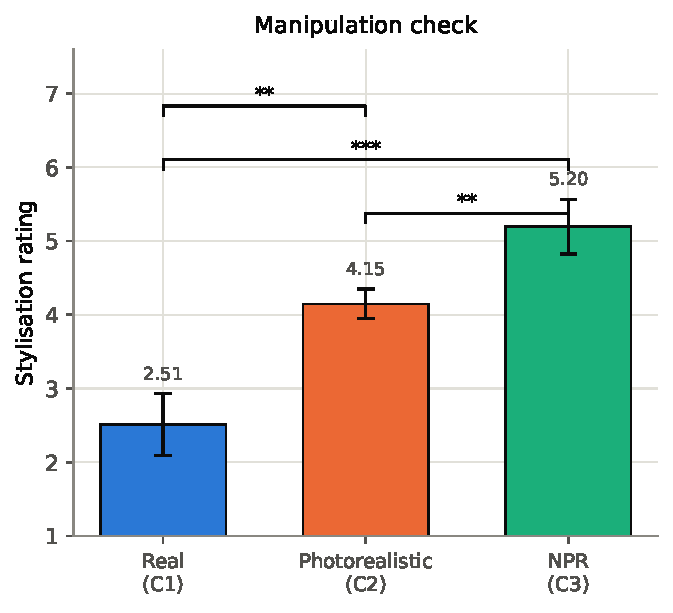
\includegraphics[height=0.40\textheight,width=0.97\textwidth,keepaspectratio]{fig_manipulation_check}\\[0.2em]
      {\tiny\color{kngrey}How stylised each advisor looked, 1 to 7.\par}
      \vspace{0.3em}
      \noindent\colorbox{knlight}{\parbox{0.96\textwidth}{\vspace{2pt}\tiny
      \setlength{\tabcolsep}{3pt}\renewcommand{\arraystretch}{1.25}
      \begin{tabular}{@{}ll@{}}
        Omnibus & $F(2,80)=15.45$, $p<.001$, $\eta^2_p=.28$ \\
        C1 vs C2 & $p=.001$, $g=0.87$ \\
        C1 vs C3 & $p<.001$, $g=1.23$ \\
        C2 vs C3 & \good{$p=.004$, $g=0.55$} \\
      \end{tabular}\vspace{2pt}}}
      \vspace{0.25em}
      {\tiny\good{All three conditions separate.}\par}
    \end{column}
  \end{columns}
\end{frame}

%% ============================================================
%% CHAPTER 6 — OUTCOMES
%% ============================================================

\begin{frame}[plain]
  \vspace{2.4em}
  \begin{center}
    \colorbox{kncyan}{\parbox{0.52\textwidth}{\centering\vspace{7pt}\fontsize{24}{28}\selectfont\bfseries\color{black} Results\vspace{7pt}}}
  \end{center}
  \vfill
  \hbox{\color{knrule}\rule{\paperwidth}{0.9pt}}
  \vspace{0.6em}
\end{frame}



\begin{frame}{H1 — Eeriness, C2 vs C3}
  \vspace{0.3em}
  \begin{columns}[T]
    \begin{column}{0.30\textwidth}
      \centering
      \vspace{0.3em}
      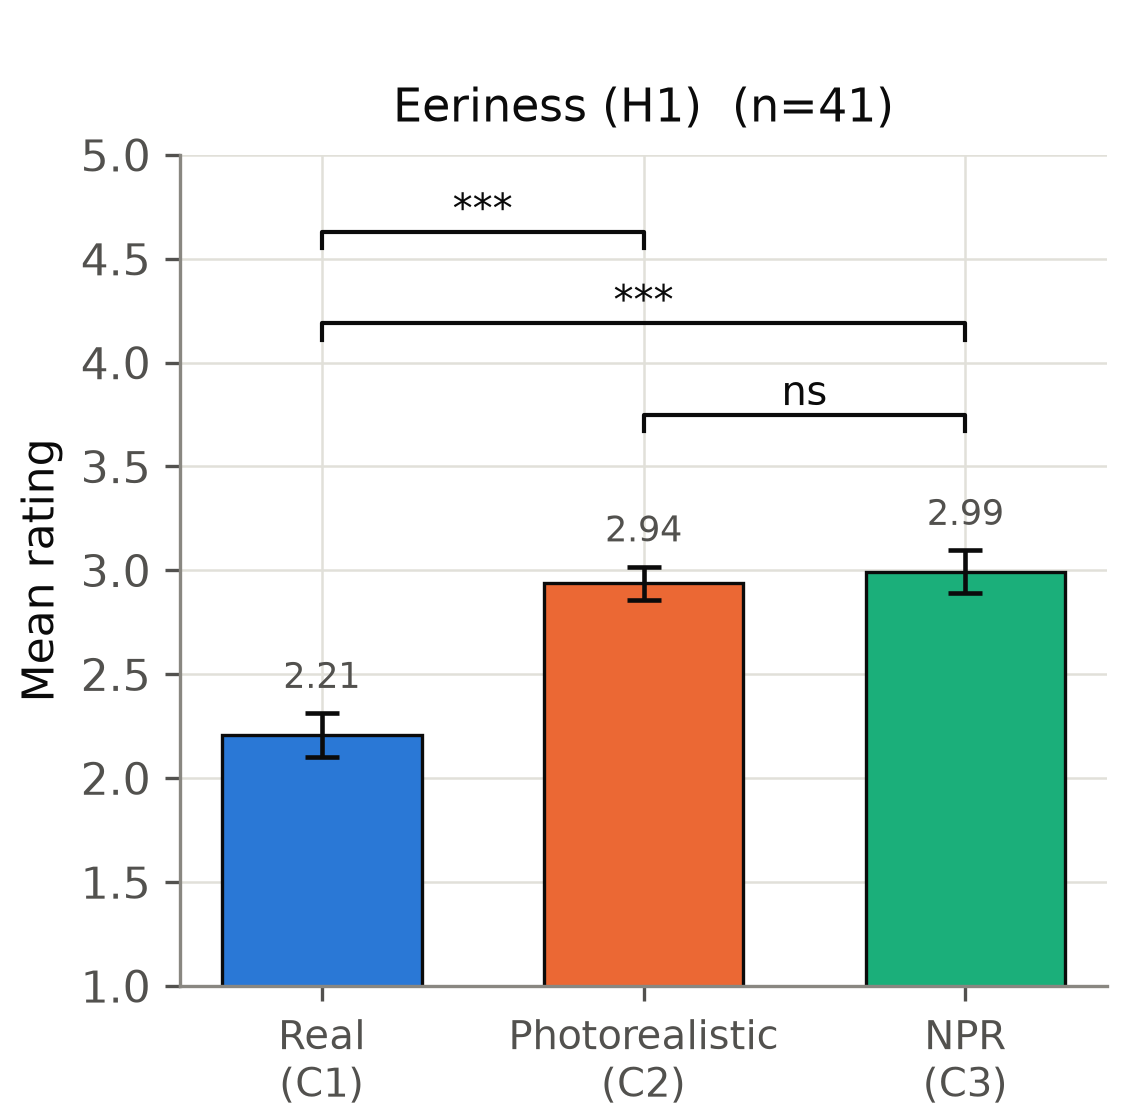
\includegraphics[width=\textwidth]{subscale_2_eeriness}
    \end{column}
    \begin{column}{0.66\textwidth}
      \vspace{0.3em}
      \begin{center}\verdict{knred}{\ H1 NOT SUPPORTED\ }\end{center}
      \vspace{0.5em}

      \scriptsize
      \begin{tabular}{@{}lccc@{}}
        \toprule
        \textbf{Eeriness} & \textbf{C1 vs C2} & \textbf{C1 vs C3} & \textbf{C2 vs C3} \\
        \midrule
        $p$ & $<.001$ & $<.001$ & \bad{$.66$} \\
        $g$ & $0.98$ & $0.98$ & \bad{$0.07$} \\
        \bottomrule
      \end{tabular}
      \vspace{0.25em}

      {\color{kngrey}\scriptsize Omnibus: $F(2,80)=20.39$, $p<.001$, $\eta^2_p=.34$\par}
      \vspace{0.7em}

      \scriptsize
      \begin{itemize}\setlength{\itemsep}{0.35em}
        \item Eeriness rose from C1 to C2 to C3, with C3 \emph{above} C2, the \hl{opposite} of the prediction
        \item Real speaker differs from both avatars
        \item The two avatars \hl{statistically indistinguishable}, $g=0.07$
        \item \hl{Stylisation and eeriness are separate effects}: seen, but not felt as less eerie
      \end{itemize}
    \end{column}
  \end{columns}
\end{frame}

\begin{frame}{H2 — Trust, C2 vs C3}
  \vspace{0.25em}
  \begin{columns}[T]
    \begin{column}{0.615\textwidth}
      \centering
      \begin{columns}[T]
        \begin{column}{0.32\textwidth}\centering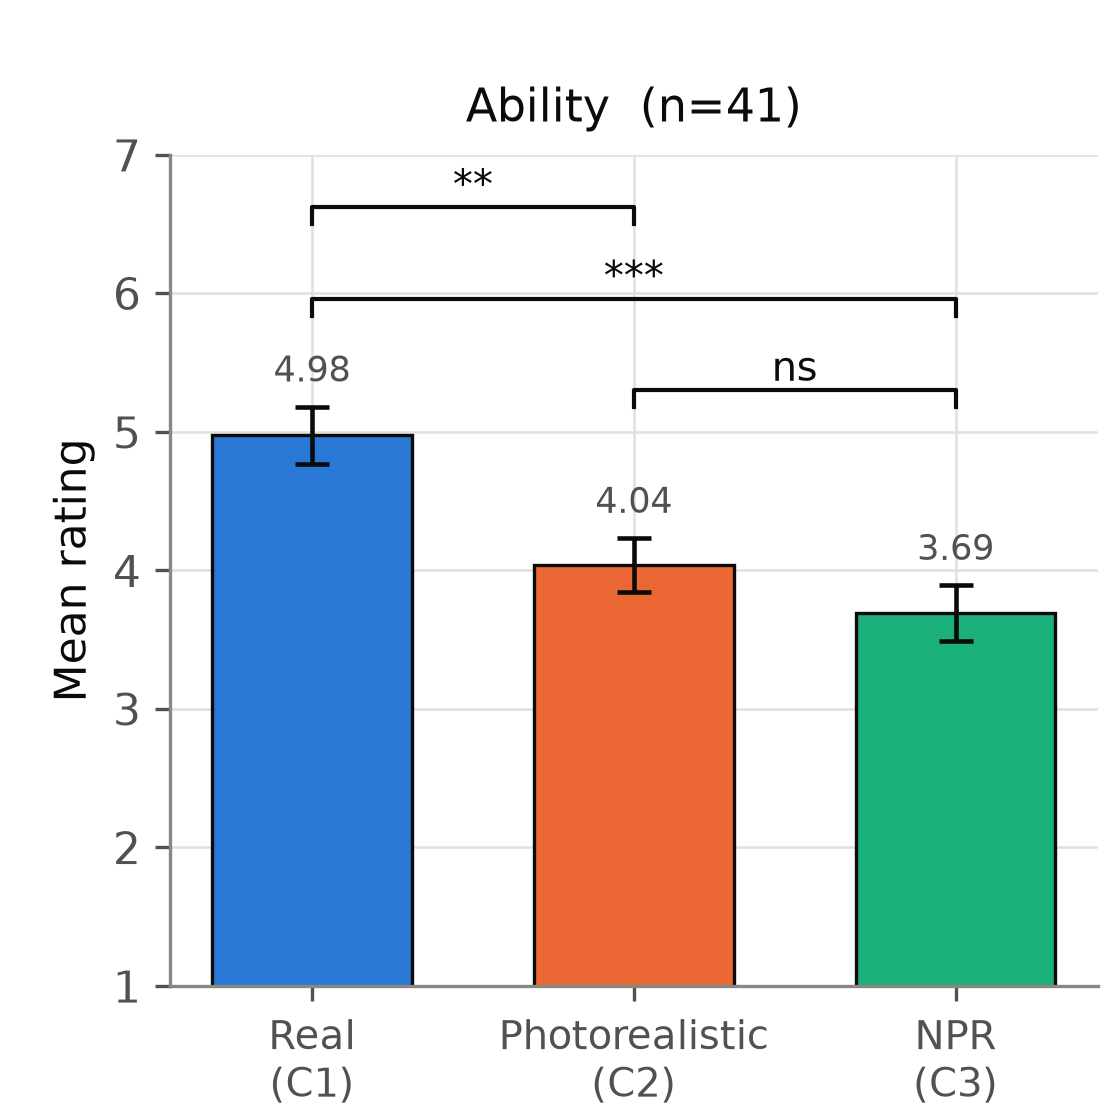
\includegraphics[width=\textwidth]{subscale_3_ability}\end{column}
        \begin{column}{0.32\textwidth}\centering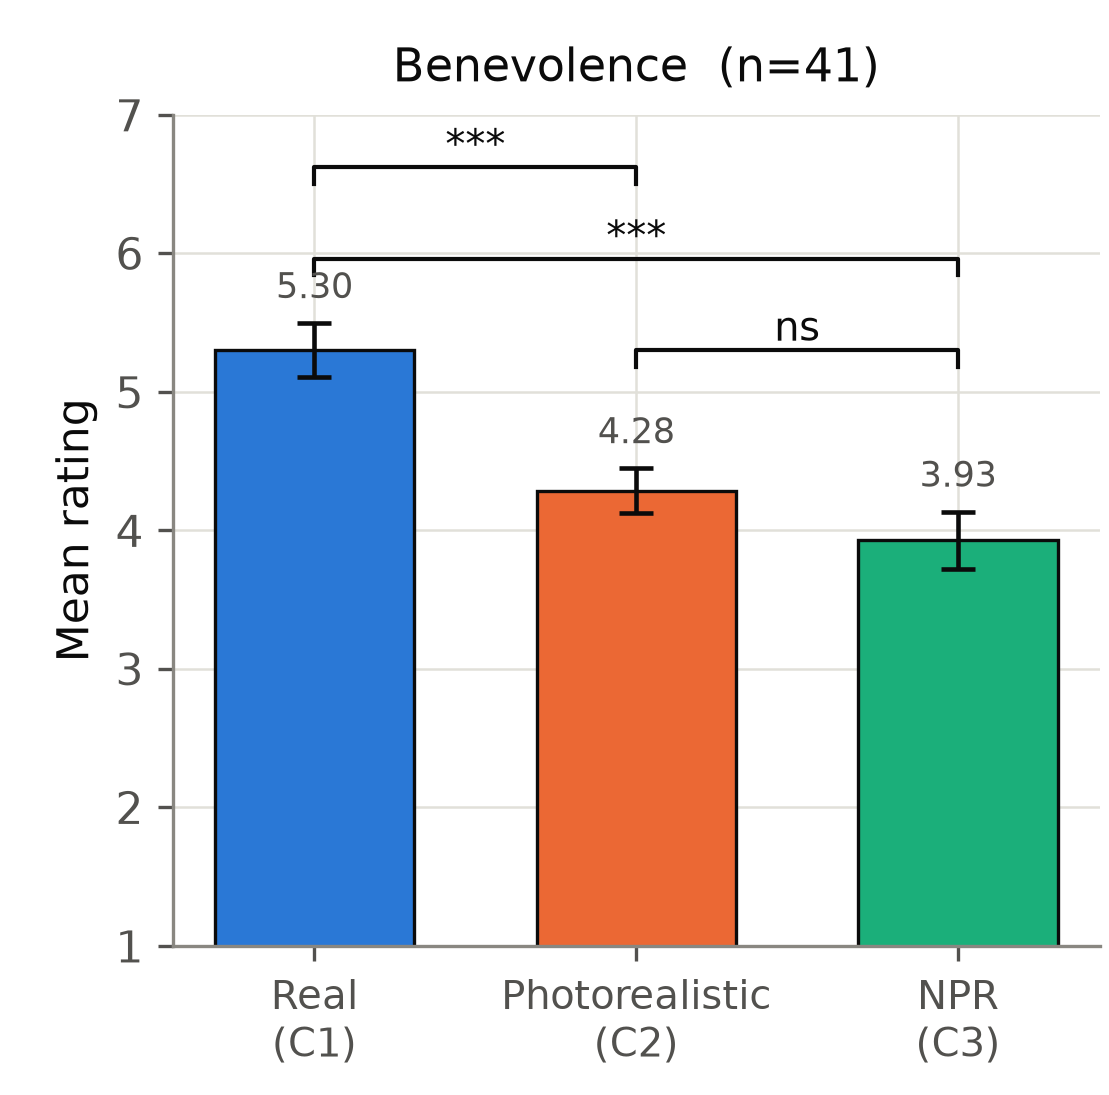
\includegraphics[width=\textwidth]{subscale_4_benevolence}\end{column}
        \begin{column}{0.32\textwidth}\centering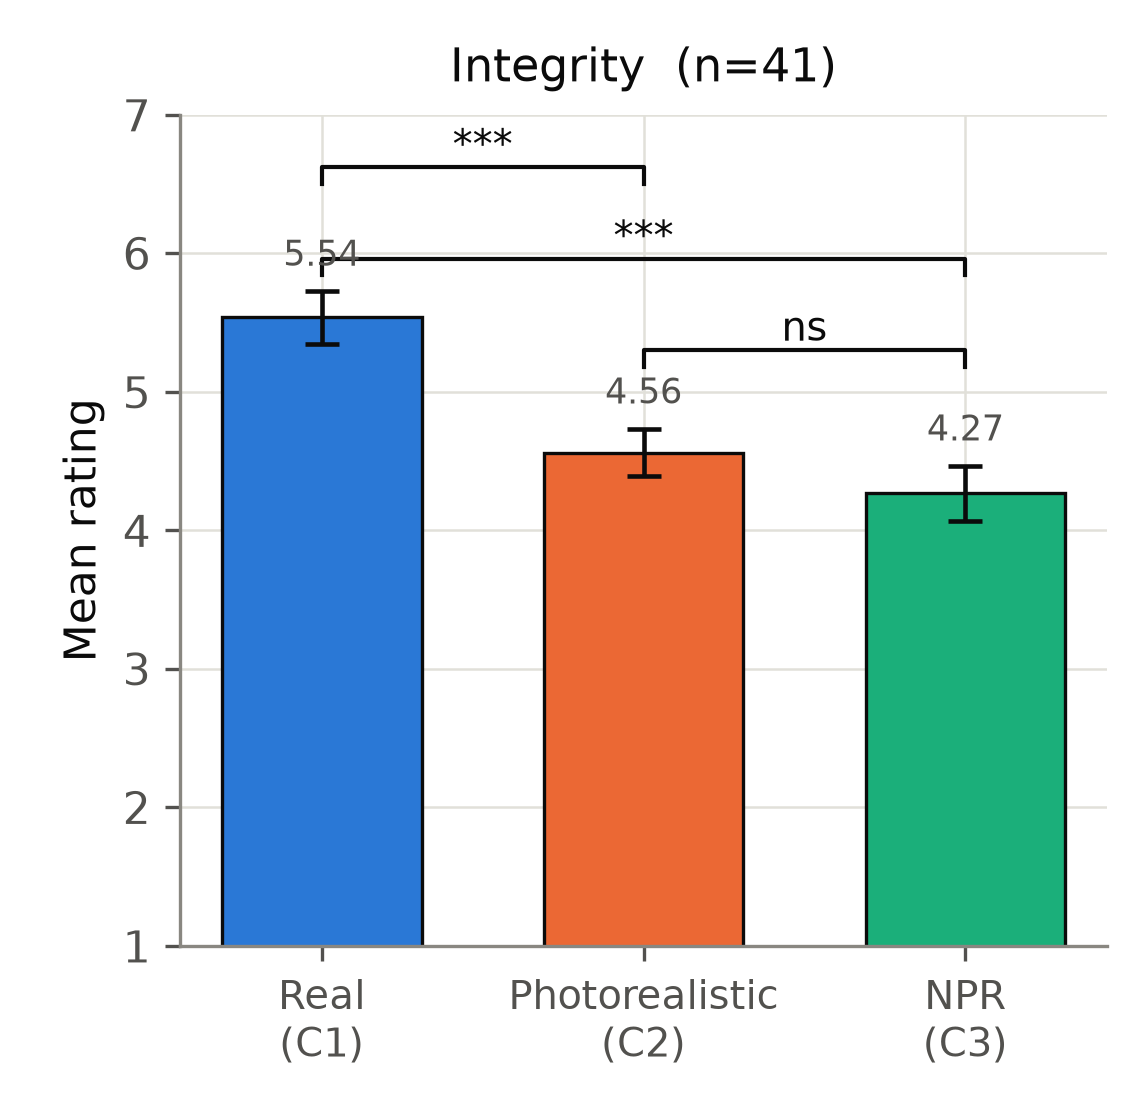
\includegraphics[width=\textwidth]{subscale_5_integrity}\end{column}
      \end{columns}
      \vspace{0.1em}

      {\tiny\color{kngrey}\textbf{ns} between the two avatars on all three trust dimensions.\par}
    \end{column}
    \begin{column}{0.355\textwidth}
      \begin{center}\verdict{kngreen}{\ H2 SUPPORTED\ }\end{center}
      \vspace{0.3em}
      \noindent\colorbox{knlight}{\parbox{0.96\textwidth}{\vspace{2pt}\tiny
      \begin{itemize}\setlength{\itemsep}{0.22em}\setlength{\leftmargini}{1.0em}
        \item \good{No statistically significant difference} across the trust subscales
        \item \bad{No difference detected}, but equivalence unestablished
        \item Realised power near $0.20$ at $n=41$
        \item Roughly \hl{three times} the sample required to separate the conditions
      \end{itemize}\vspace{2pt}}}
    \end{column}
  \end{columns}
  \vspace{0.5em}

  \begin{columns}[c]
    \begin{column}{0.26\textwidth}
      \scriptsize
      \textbf{Step 1. Pairwise, C2 vs C3}
      \vspace{0.2em}

      \begin{tabular}{@{}lcc@{}}
        \toprule
        & $p$ & $g$ \\
        \midrule
        Ability      & $.21$ & $0.20$ \\
        Benevolence  & $.18$ & $0.19$ \\
        Integrity    & $.27$ & $0.16$ \\
        \bottomrule
      \end{tabular}
    \end{column}
    \begin{column}{0.30\textwidth}
      \scriptsize
      \textbf{Step 2. TOST, trust composite}
      \vspace{0.2em}

      \begin{tabular}{@{}lccc@{}}
        \toprule
        & Diff. & Bound & TOST $p$ \\
        \midrule
        C2 vs C3 & $0.33$ & $\pm0.51$ & \bad{$.240$} \\
        \bottomrule
      \end{tabular}
    \end{column}
    \begin{column}{0.40\textwidth}
      \centering
      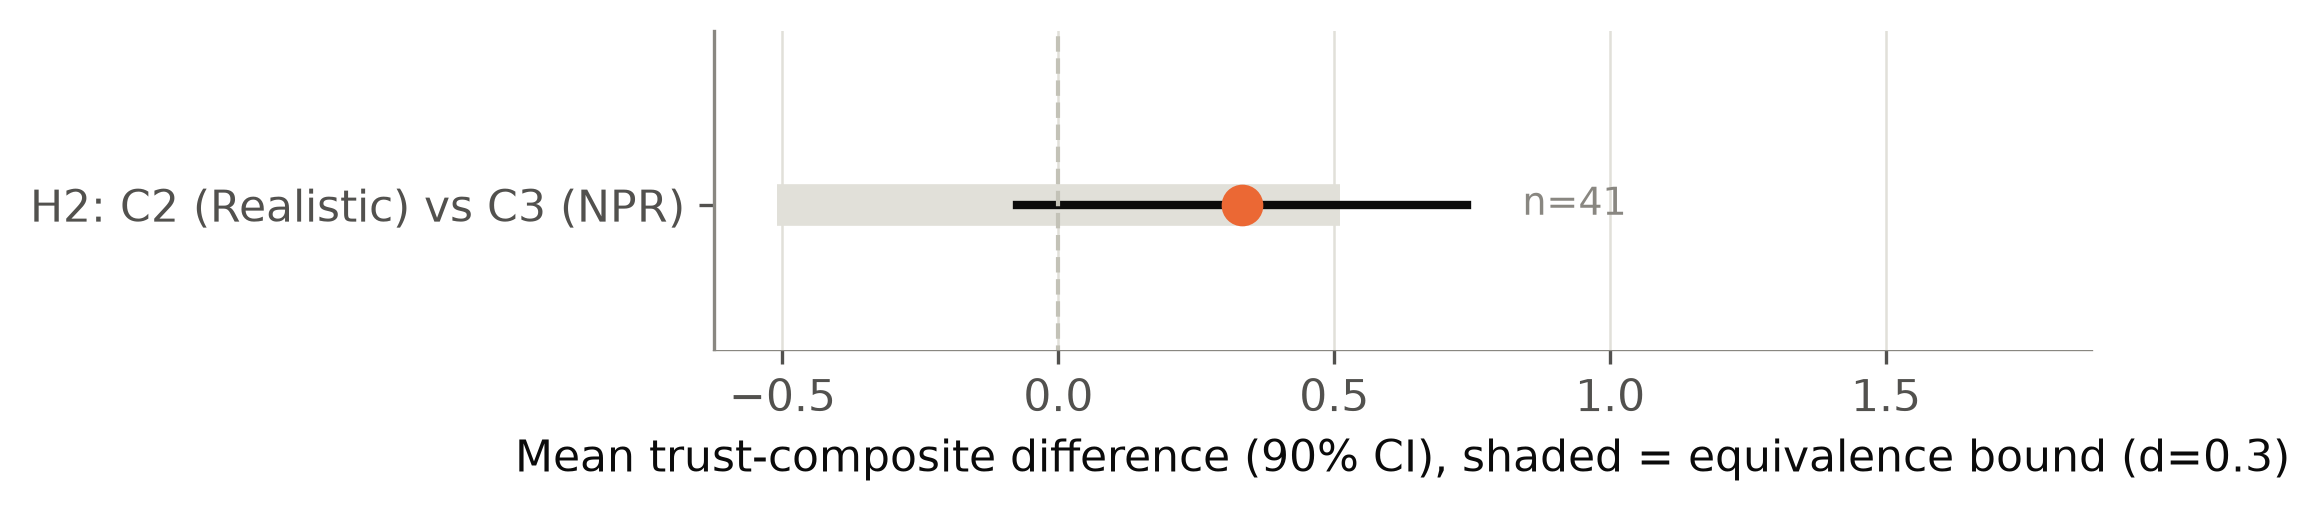
\includegraphics[width=\textwidth]{tost_H2_row}
    \end{column}
  \end{columns}
\end{frame}

\begin{frame}{H3 — Eeriness, likeability and trust}
  \vspace{0.2em}
  \begin{columns}[T]
    \begin{column}{0.60\textwidth}
      \centering
      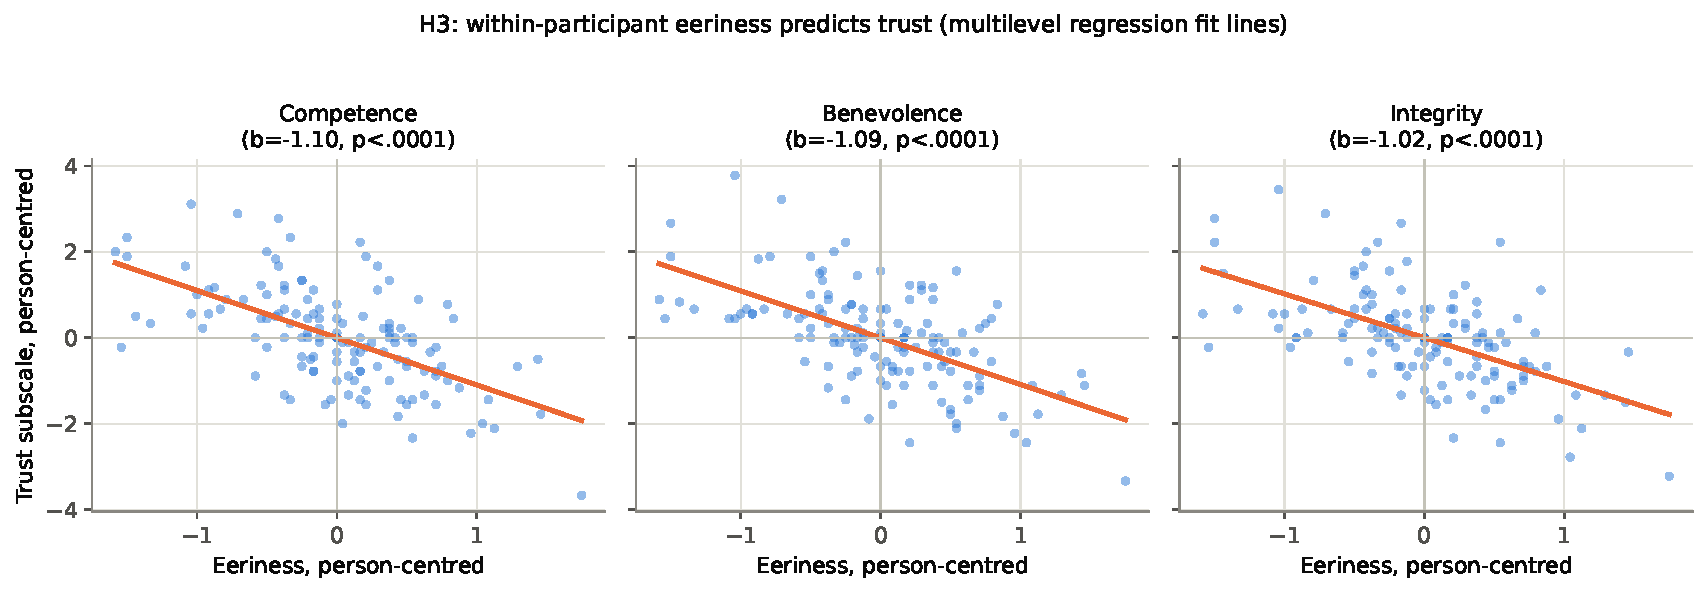
\includegraphics[height=0.50\textheight]{fig_h3_eeriness_trust}
    \end{column}
    \begin{column}{0.38\textwidth}
      \vspace{0.2em}
      \begin{center}\verdict{kngreen}{\ H3 CONFIRMED\ }\end{center}
      \vspace{0.4em}

      \noindent\colorbox{knlight}{\parbox{0.96\textwidth}{\vspace{2pt}\scriptsize
      \begin{itemize}\setlength{\itemsep}{0.18em}\setlength{\leftmargini}{1.0em}
        \item \hl{Within} participants, not between conditions
        \item Eeriness \bad{lowers} trust, likeability \good{raises} it
        \item About \hl{one point for one point}, on every dimension
        \item Confirmed in \hl{both} directions
        \item Caveat: the two correlate at $r=-.72$, and cannot be separated cleanly here
      \end{itemize}\vspace{2pt}}}
      \vspace{0.3em}

      \scriptsize
      \begin{tabular}{@{}lcc@{}}
        \toprule
        \textbf{Predictor} & \textbf{Eeriness} & \textbf{Likeability} \\
        \midrule
        Ability      & $-1.17$ & $+1.10$ \\
        Benevolence  & $-1.10$ & $+1.10$ \\
        Integrity    & $-1.02$ & $+1.08$ \\
        \bottomrule
      \end{tabular}\\[0.2em]
      {\color{kngrey}\scriptsize Fixed-effect slopes, all $p<.001$}
    \end{column}
  \end{columns}
\end{frame}

\begin{frame}{H4 — Trust, C1 vs C3}
  \vspace{0.25em}
  \begin{columns}[T]
    \begin{column}{0.615\textwidth}
      \centering
      \begin{columns}[T]
        \begin{column}{0.32\textwidth}\centering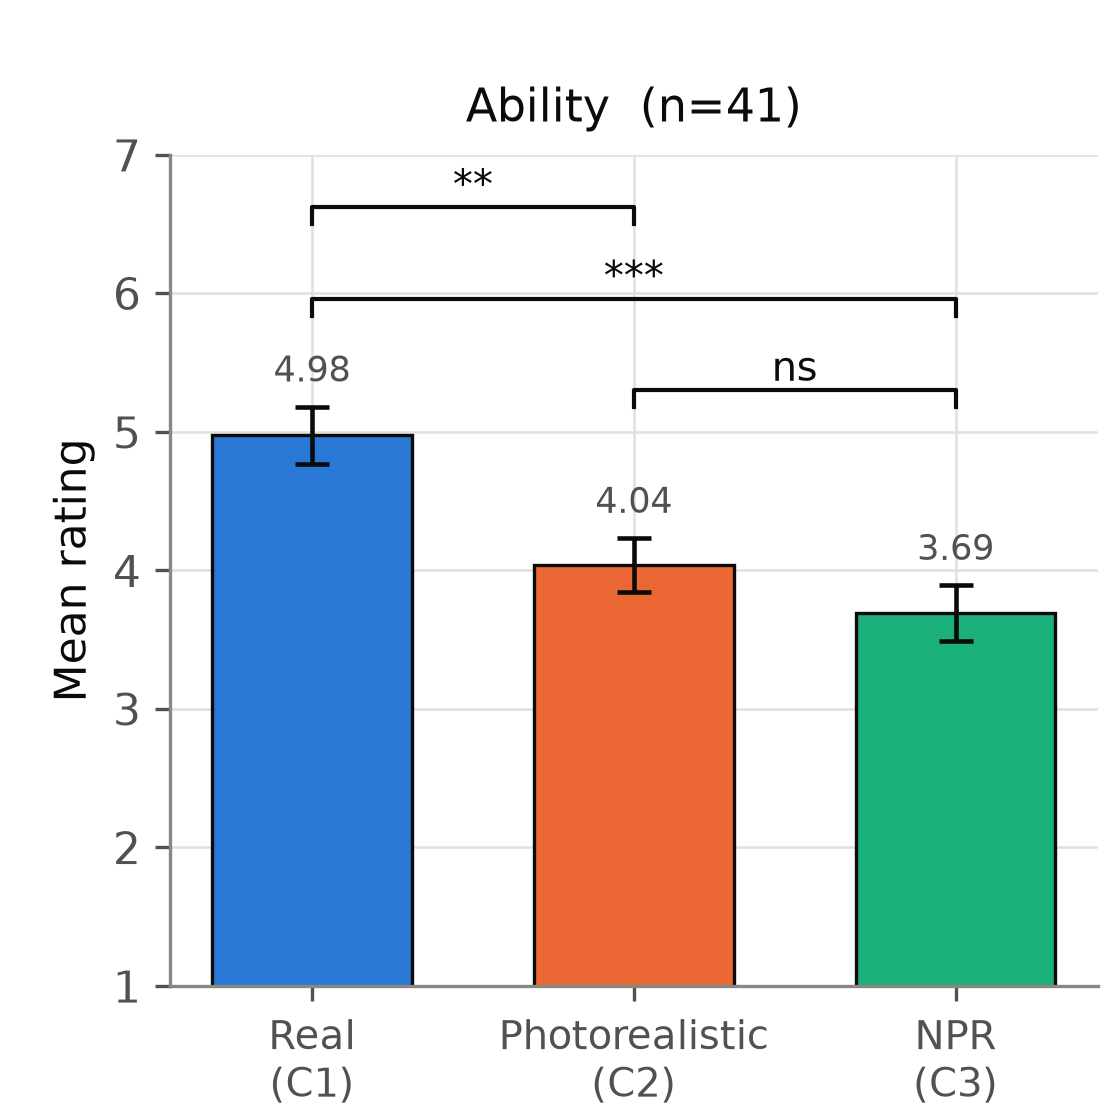
\includegraphics[width=\textwidth]{subscale_3_ability}\end{column}
        \begin{column}{0.32\textwidth}\centering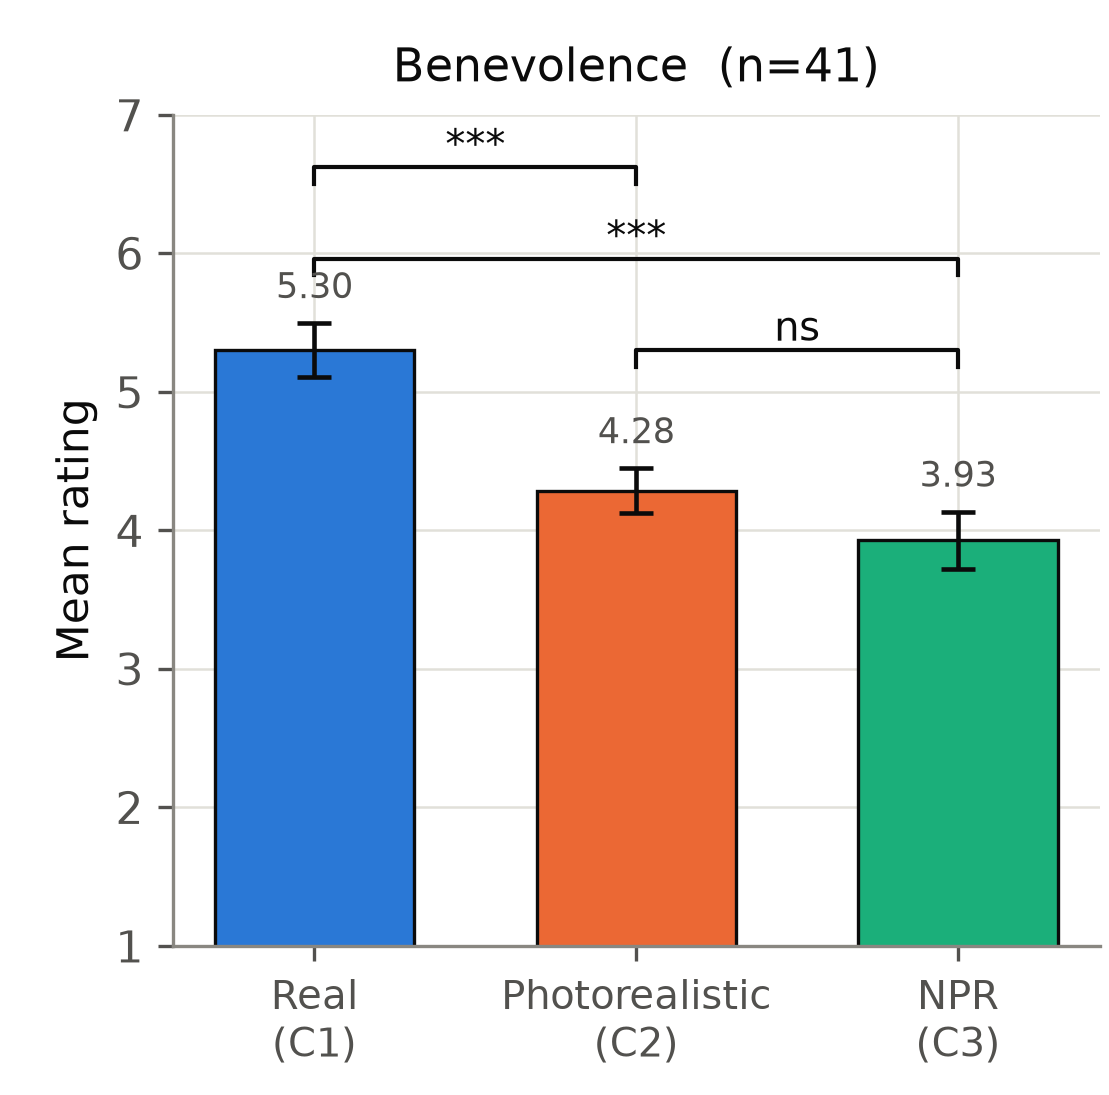
\includegraphics[width=\textwidth]{subscale_4_benevolence}\end{column}
        \begin{column}{0.32\textwidth}\centering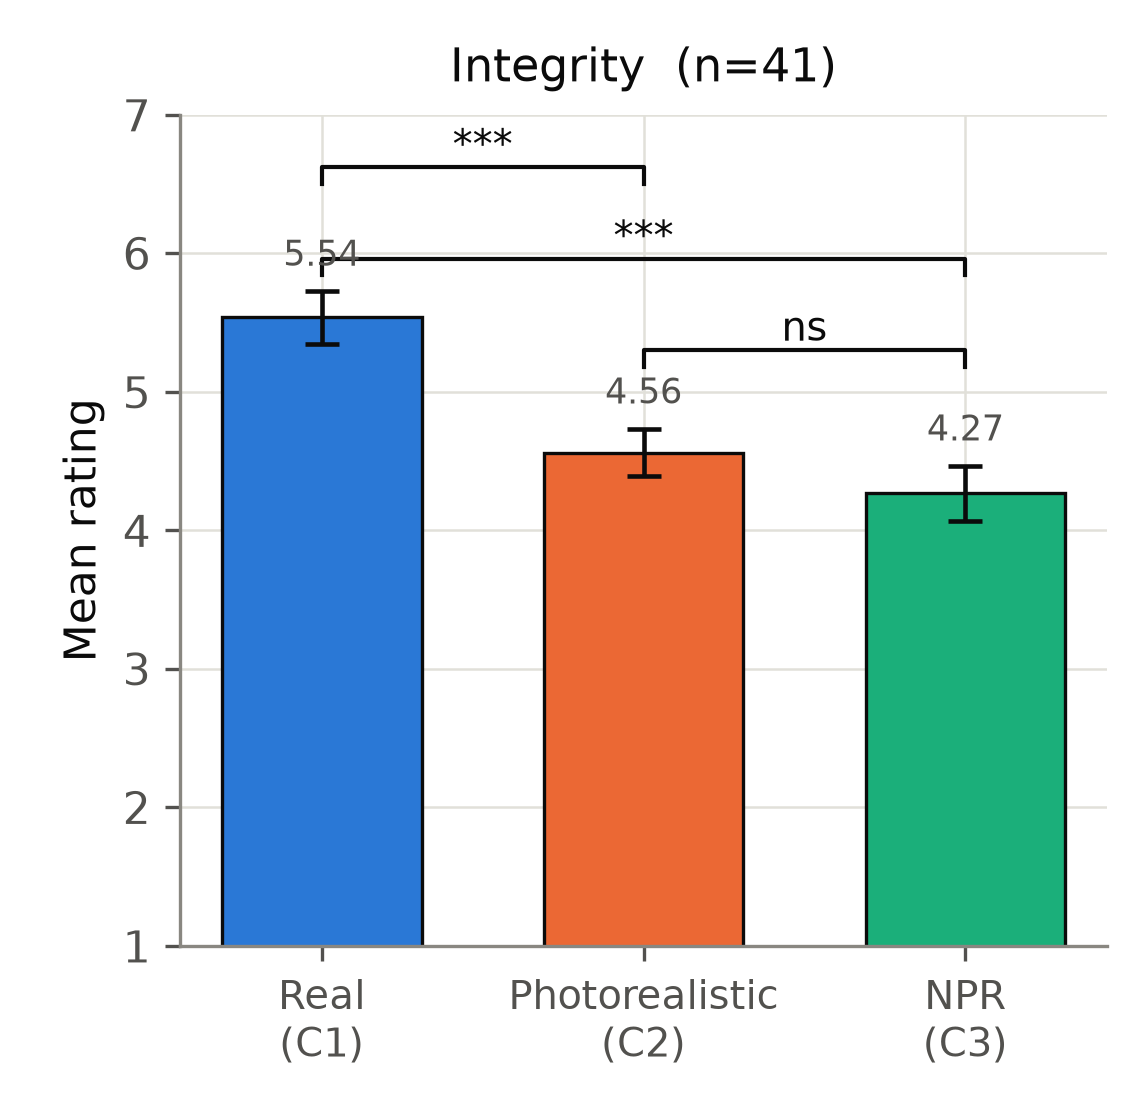
\includegraphics[width=\textwidth]{subscale_5_integrity}\end{column}
      \end{columns}
      \vspace{0.1em}

      {\tiny\color{kngrey}The real speaker is \textbf{significantly above} the NPR avatar on all three.\par}
    \end{column}
    \begin{column}{0.355\textwidth}
      \begin{center}\verdict{knred}{\ H4 NOT SUPPORTED\ }\end{center}
      \vspace{0.3em}
      \noindent\colorbox{knlight}{\parbox{0.96\textwidth}{\vspace{2pt}\tiny
      \begin{itemize}\setlength{\itemsep}{0.22em}\setlength{\leftmargini}{1.0em}
        \item All three subscales \hl{significantly higher} for the real speaker
        \item Nearly \hl{three times} the equivalence bound
        \item Not a marginal shortfall
        \item Two explanations stay open: the uncanny valley, or participants recognising the speaker
      \end{itemize}\vspace{2pt}}}
    \end{column}
  \end{columns}
  \vspace{0.5em}

  \begin{columns}[c]
    \begin{column}{0.26\textwidth}
      \scriptsize
      \textbf{Step 1. Pairwise, C1 vs C3}
      \vspace{0.2em}

      \begin{tabular}{@{}lcc@{}}
        \toprule
        & $p$ & $g$ \\
        \midrule
        Ability      & $<.001$ & $0.75$ \\
        Benevolence  & $<.001$ & $0.79$ \\
        Integrity    & $<.001$ & $0.80$ \\
        \bottomrule
      \end{tabular}
    \end{column}
    \begin{column}{0.30\textwidth}
      \scriptsize
      \textbf{Step 2. TOST, trust composite}
      \vspace{0.2em}

      \begin{tabular}{@{}lccc@{}}
        \toprule
        & Diff. & Bound & TOST $p$ \\
        \midrule
        C1 vs C3 & \bad{$1.31$} & $\pm0.47$ & $.998$ \\
        \bottomrule
      \end{tabular}
    \end{column}
    \begin{column}{0.40\textwidth}
      \centering
      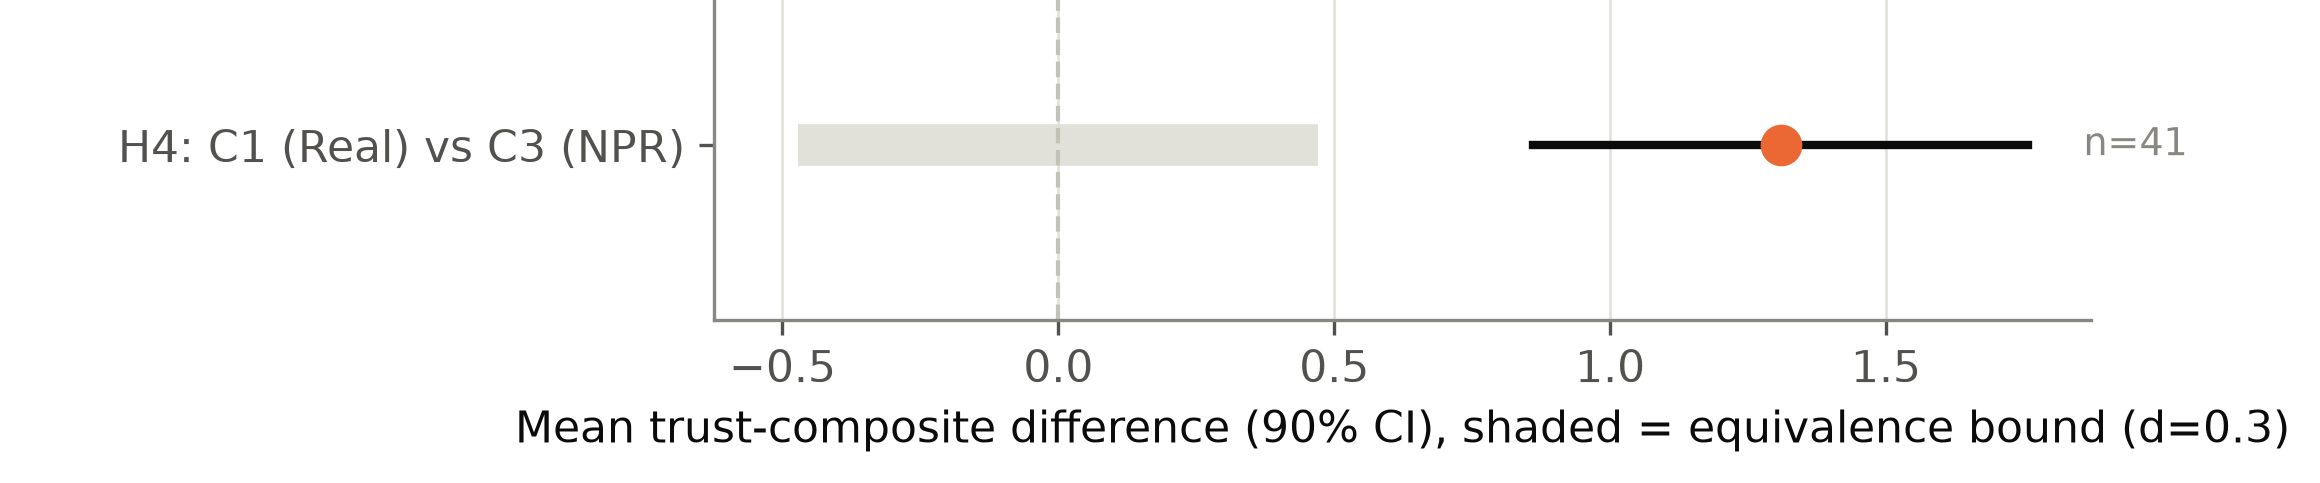
\includegraphics[width=\textwidth]{tost_H4_row}
    \end{column}
  \end{columns}
\end{frame}

\begin{frame}{The Behavioural Measure}{Chapter 6.2.6 — the three rankings}
  \vspace{0.2em}
  \centering
  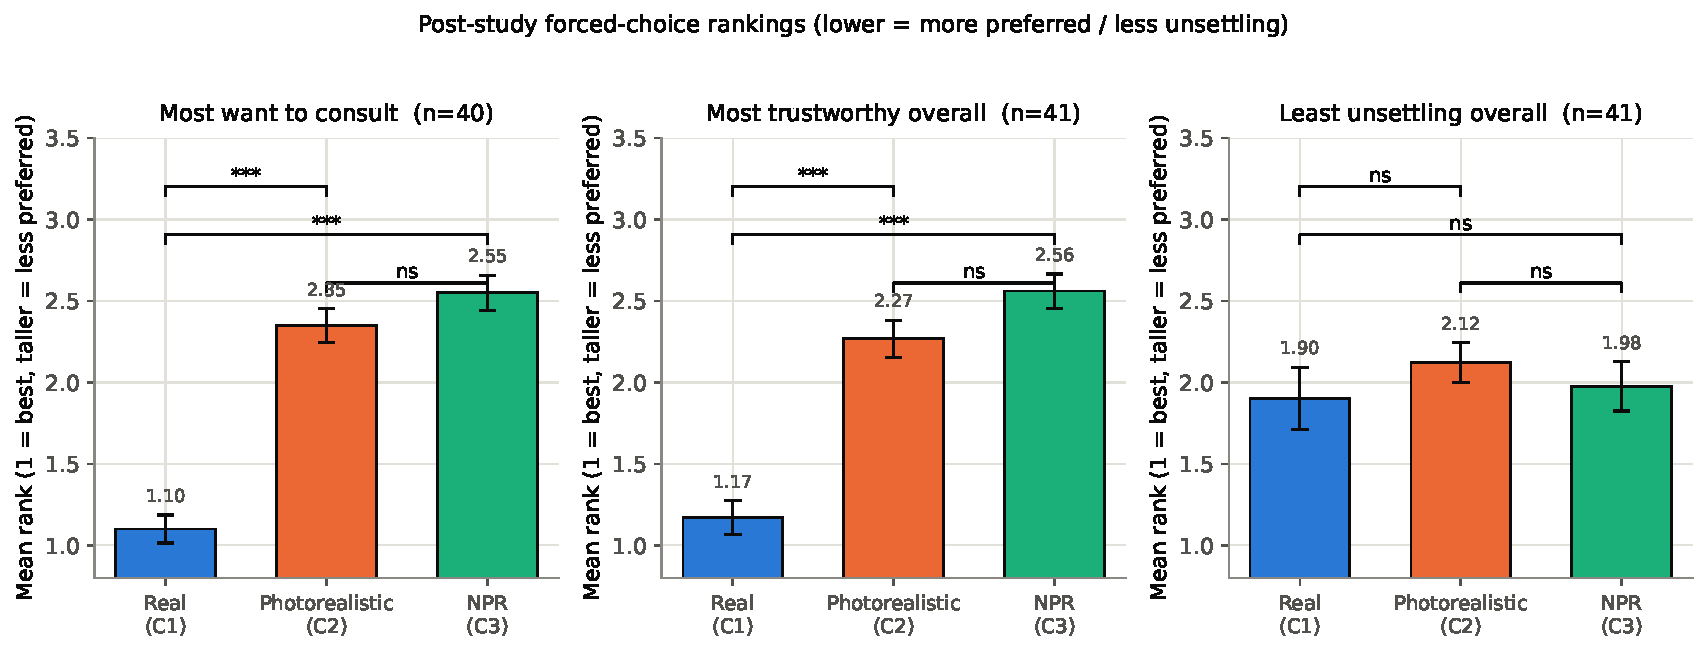
\includegraphics[height=0.39\textheight]{fig_rankings}
  \vspace{0.3em}

  {\scriptsize
  \setlength{\tabcolsep}{5pt}\renewcommand{\arraystretch}{1.2}
  \begin{tabular}{@{}llll@{}}
    \toprule
    \textbf{Question} & \textbf{Friedman} & \textbf{C1 vs C2/C3} & \textbf{C2 vs C3} \\
    \midrule
    Most want to consult & $\chi^2_F(2)=49.40$, $p<.001$ & $p<.001$ & $p=.21$ \\
    Most trustworthy     & $\chi^2_F(2)=44.05$, $p<.001$ & $p<.001$ & $p=.07$ \\
    Least unsettling     & $\chi^2_F(2)=1.02$, $p=.60$   & $p=.97$  & $p=.97$ \\
    \bottomrule
  \end{tabular}\par}
  \vspace{0.3em}
  {\scriptsize\color{knblue}\textbf{Lower is better} — rank 1 = most preferred.\par}
  \vspace{0.3em}
  \colorbox{knlight}{\parbox{0.6\textwidth}{\centering\vspace{2pt}\scriptsize\color{knblue}
  The real speaker ranks first. The \textbf{two avatars tie}.\vspace{2pt}}}
\end{frame}


%% ============================================================
%% DISCUSSION, LIMITATIONS, CONCLUSION
%% ============================================================

\begin{frame}{RQ3 Answer}{What stylisation did to eeriness and trustworthiness, and how far it reached}
  \vspace{0.45em}
  \begin{columns}[T]
    \begin{column}{0.315\textwidth}
      \panelhead{What Did Not Happen}
      \panel{%
        \item Eeriness \bad{did not fall}, it rose slightly
        \item The two avatars \hl{indistinguishable} on all five subscales
        \item No behavioural advantage either}
    \end{column}
    \begin{column}{0.315\textwidth}
      \panelhead{What Did Happen}
      \panel{%
        \item \good{No trust penalty} detected for stylisation
        \item Within a person, eeriness \bad{lowers} trust and likeability \good{raises} it
        \item About \hl{one point for one point}, on all three trust dimensions
        \item The route from appearance to trust is real, the composite just never used it}
    \end{column}
    \begin{column}{0.315\textwidth}
      \panelhead{The Dividing Line}
      \panel{%
        \item The gap is \hl{not between render styles}
        \item C2 vs C3: $0.33$ points, inside the noise
        \item C1 vs C3: \bad{$1.31$ points}, nearly three times the bound}
    \end{column}
  \end{columns}
  \vfill
  \begin{center}
    \setlength{\tabcolsep}{10pt}\renewcommand{\arraystretch}{1.0}
    \begin{tabular}{@{}ccc@{}}
      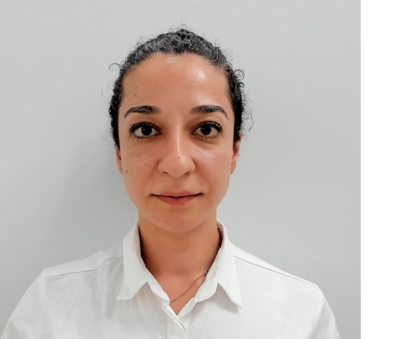
\includegraphics[height=1.35cm,keepaspectratio]{stimulus_C1_real} &
      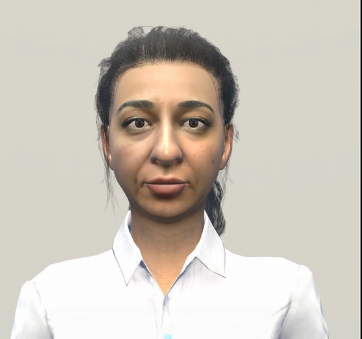
\includegraphics[height=1.35cm,keepaspectratio]{stimulus_C2_photorealistic} &
      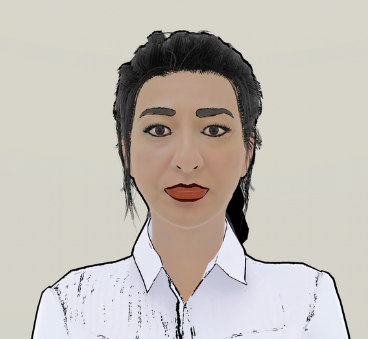
\includegraphics[height=1.35cm,keepaspectratio]{stimulus_C3_npr} \\[0.1em]
      {\tiny\color{kngrey}C1 — Real} &
      {\tiny\color{kngrey}C2 — Photorealistic} &
      {\tiny\color{kngrey}C3 — NPR} \\
    \end{tabular}
  \end{center}
\end{frame}

\begin{frame}[plain]
  \vspace{2.4em}
  \begin{center}
    \colorbox{kncyan}{\parbox{0.58\textwidth}{\centering\vspace{7pt}\fontsize{24}{28}\selectfont\bfseries\color{black} Discussion\vspace{7pt}}}
  \end{center}
  \vfill
  \hbox{\color{knrule}\rule{\paperwidth}{0.9pt}}
  \vspace{0.6em}
\end{frame}

\begin{frame}{Why the two avatars scored the same}{Two mismatches inside the composite}
  \vspace{0.3em}
  \begin{columns}[T,onlytextwidth]
    \begin{column}{\textwidth}
      \panelhead{What Needs Explaining}
      \panel{%
        \item Real speaker \bad{far above} both avatars
        \item The two avatars: \hl{seen as different}, \hl{scored the same}
        \item H3: appearance \good{moves trust}, but the composite never used that route}
    \end{column}
  \end{columns}
  \par\vspace*{1.6em}
  \begin{columns}[T,onlytextwidth]
    \begin{column}{0.485\textwidth}
      \panelhead{1. Material vs.\ Shape}
      \panel{%
        \item The composite stylises the \hl{material}, not the \hl{shape}
        \item Zell et al.\ 2015: eeriness \bad{rises} when material and shape disagree~[15]
        \item Stronger stylisation would only \bad{widen} the gap}
    \end{column}
    \begin{column}{0.485\textwidth}
      \panelhead{2. Appearance vs.\ Performance}
      \panel{%
        \item Both avatars share the \hl{same} recorded voice and animation
        \item C3 puts a \hl{human performance} on an abstracted face
        \item Cihodaru 2025, K\"atsyri et al.\ 2015: mismatched human likeness is \bad{rated eerier}~[16,\,17]}
    \end{column}
  \end{columns}
\end{frame}

\begin{frame}{What this design could not show}{Chapter 6.3 — four factors this design cannot rule out}
  \vspace{0.1em}
  \begin{columns}[T,onlytextwidth]
    \begin{column}{0.485\textwidth}
      \panelhead{1. The Comparison Set}
      \panel{%
        \item Real speaker sets the top: only \hl{how far below?}
        \item Rendering gap vs.\ \hl{human versus CG} gap
        \item Fits the tiny C2--C3 likeability and eeriness gap
        \item C3 right after C1 in 2 of 3 versions, C2 \bad{never}
        \item Without C1, abstraction is the \hl{only axis}}
    \end{column}
    \begin{column}{0.485\textwidth}
      \panelhead{2. Familiarity with the Speaker}
      \panel{%
        \item C1 is \hl{the researcher}
        \item Recognition adds trust \bad{no rendering can match}
        \item Lifts C1 above a stranger, widening the gap
        \item No recognition item: share \bad{unknown}}
    \end{column}
  \end{columns}
  \par\vspace*{0.6em}
  \begin{columns}[T,onlytextwidth]
    \begin{column}{0.485\textwidth}
      \panelhead{3. The Video Setting}
      \panel{%
        \item Flat, prerecorded, \hl{no interaction}
        \item Zibrek \& McDonnell 2019: in VR, realism raised \hl{presence}~[18]
        \item Interaction lets mismatches show more
        \item VR \hl{may separate} C2 and C3}
    \end{column}
    \begin{column}{0.485\textwidth}
      \panelhead{4. Expectations of Generative Video}
      \panel{%
        \item One participant asked \hl{which AI} made the videos
        \item One remark: an \hl{observation}, not a result
        \item AI doubt lowers \bad{both} avatars equally
        \item Nobody was told the videos were \hl{not} AI}
    \end{column}
  \end{columns}
\end{frame}

\begin{frame}{Limitations}{Five, and each one bounds a different claim}
  \vspace{0.2em}
  \begin{columns}[T]
    \begin{column}{0.315\textwidth}
      \panelhead{Session Length}
      \panel{%
        \item 10 to 15 minutes per study
        \item Every measure completed \hl{three times}
        \item Capped the measures and the breadth of the design}
    \end{column}
    \begin{column}{0.315\textwidth}
      \panelhead{One Configuration}
      \panel{%
        \item One composite, one avatar, one platform, three scenarios
        \item Characterises \hl{this configuration}, not NPR as a category}
    \end{column}
    \begin{column}{0.315\textwidth}
      \panelhead{Parameter Study Scope}
      \panel{%
        \item Only the \hl{most influential} parameters tested
        \item The rest fixed by inspection in development
        \item Highest \bad{among those tested}, not necessarily the best available}
    \end{column}
  \end{columns}
  \vspace{0.35em}

  \begin{columns}[T]
    \begin{column}{0.315\textwidth}
      \panelhead{Sample Size}
      \panel{%
        \item Deadline set the collection window, in the semester break
        \item $n=41$ \good{detects} a difference
        \item \bad{Not} the far larger sample equivalence demands}
    \end{column}
    \begin{column}{0.315\textwidth}
      \panelhead{Counterbalancing}
      \panel{%
        \item \hl{Full} balancing of three conditions needs all \hl{six} orders
        \item Six would have demanded about \hl{twice} the sample
        \item A Latin square with \hl{three} was used instead}
    \end{column}
  \end{columns}
\end{frame}

\begin{frame}{Conclusion}{What was built, what it showed, and what it means}
  \vspace{0.5em}
  \begin{columns}[T]
    \begin{column}{0.315\textwidth}
      \panelhead{What This Thesis Built}
      \panel{%
        \item NPR stylisation for \hl{Mixamo, the Meta SDK and Avaturn}
        \item Eight techniques in sequence, each answering a limitation of the one before
        \item Narrowed to \hl{three} by visual assessment and a parameter adjustment study}
    \end{column}
    \begin{column}{0.315\textwidth}
      \panelhead{What the Study Showed}
      \panel{%
        \item The composite \bad{did not reduce eeriness} against the photorealistic baseline
        \item It produced \good{no observed trust penalty} either
        \item The evidence does not indicate stylisation reduced trust
        \item It is \bad{not sufficient} to establish that the two are equivalent}
    \end{column}
    \begin{column}{0.315\textwidth}
      \panelhead{What It Means}
      \panel{%
        \item A developer choosing between the two styles need not assume \good{an inherent disadvantage}
        \item The gap that matters is \bad{not between render styles}
        \item It is the distance to the \hl{real human}, and neither avatar closed any part of it}
    \end{column}
  \end{columns}
  \vfill
  \noindent\colorbox{knlight}{\parbox{0.975\textwidth}{\centering\color{knblue}\scriptsize
  \textbf{Reaching the credibility of an actual human is a harder challenge than selecting a rendering style.}\\
  It is also the problem that decides whether virtual advisors become genuinely trusted participants rather than a passing novelty.}}
\end{frame}

\begin{frame}{Future work}{Six steps, in the order the thesis sets them out}
  \vspace{0.6em}
  \begin{columns}[T,onlytextwidth]
    \begin{column}{0.158\textwidth}
      \panelheadsm{1. Larger Replication}
      \panel{%
        \item Repeat C2 versus C3 with roughly \hl{120 participants}
        \item Settles the equivalence question either way}
    \end{column}
    \begin{column}{0.158\textwidth}
      \panelheadsm{2. Stylise the Geometry}
      \panel{%
        \item Shift proportion and feature scale \hl{alongside the shading}
        \item Tests the material-versus-shape mismatch
        \item Match \hl{voice and motion} to the stylised face}
    \end{column}
    \begin{column}{0.158\textwidth}
      \panelheadsm{3. Drop the Real Speaker}
      \panel{%
        \item Removes the human \hl{anchor}
        \item Shows whether the two avatars separate with no human in view}
    \end{column}
    \begin{column}{0.158\textwidth}
      \panelheadsm{4. Rule Out Generative AI}
      \panel{%
        \item State at the outset that the videos were \hl{not AI-generated}
        \item That belief may have lowered trust for both avatars}
    \end{column}
    \begin{column}{0.158\textwidth}
      \panelheadsm{5. Sweep Abstraction}
      \panel{%
        \item Replace the single point with a \hl{curve}
        \item Can reveal an optimum between full realism and full abstraction}
    \end{column}
    \begin{column}{0.158\textwidth}
      \panelheadsm{6. Restore Interaction}
      \panel{%
        \item Reciprocal behaviour and shared space, in \hl{VR}
        \item Across multiple avatar identities and platforms}
    \end{column}
  \end{columns}
\end{frame}
\begin{frame}[plain]
  \vspace{2.2em}
  \begin{center}
    {\LARGE\bfseries\color{knblue} Thank you}\\[1.2em]
    {\large\color{kngrey} Questions}\\[2.0em]
    \colorbox{knlight}{\parbox{0.78\textwidth}{\centering\color{knblue}\small
    Eight NPR techniques, three avatar platforms, two studies, 86 participants.\\[0.6em]
    Stylisation was clearly seen, cost no measurable trust,\\ and did not close the gap to a real human.}}\\[1.6em]
    {\footnotesize\color{kngrey} Nidanur Günay \quad|\quad nidanur.guenay@uni-konstanz.de}
  \end{center}
\end{frame}

%% ============================================================
%% 27 — References
%% ============================================================


\begin{frame}{References}
  \vspace{0.2em}
  \tiny
  \begin{columns}[T]
    \begin{column}{0.325\textwidth}
      [1] Mori, M. The Uncanny Valley. \textit{Energy} 7(4), 33--35, 1970.\\[0.3em]
      [2] MacDorman, K.\,F., Ishiguro, H. The Uncanny Advantage of Using Androids in Cognitive and Social Science Research. \textit{Interaction Studies} 7(3), 297--337, 2006.\\[0.3em]
      [3] Ho, C.-C., MacDorman, K.\,F. Revisiting the Uncanny Valley Theory. \textit{Computers in Human Behavior} 26(6), 1508--1518, 2010.\\[0.3em]
      [4] Dill, V.\ et al. Evaluation of the Uncanny Valley in CG Characters. \textit{IVA 2012}, 511--513.\\[0.3em]
      [5] Nowak, K.\,L., Rauh, C. The Influence of the Avatar on Online Perceptions of Anthropomorphism, Androgyny, Credibility, Homophily, and Attraction. \textit{JCMC} 11(1), 153--178, 2005.\\[0.3em]
      [6] Mayer, R.\,C., Davis, J.\,H., Schoorman, F.\,D. An Integrative Model of Organizational Trust. \textit{AMR} 20(3), 709--734, 1995.\\[0.3em]
      [7] Canales, R., Roble, D., Neff, M. The Impact of Avatar Stylization on Trust. \textit{IEEE VR}, 418--428, 2024.\\[0.3em]
      [8] Dubosc, C.\ et al. Effect of Avatar Stylization and Facial Expression Intensity in Virtual Interactions. \textit{Virtual Reality} 29(4), 2025.\\[0.3em]
      [9] Gao, Y.\ et al. Trust in Virtual Agents: Exploring the Role of Stylization and Voice. \textit{IEEE TVCG} 31(5), 3623--3633, 2025.\\[0.3em]
    \end{column}
    \begin{column}{0.325\textwidth}
      [10] Tao, Z.\ et al. Impact of Virtual Avatar Appearance Realism. \textit{Frontiers in Psychology} 16, 2025.\\[0.3em]
      [11] Adobe Inc. Mixamo: 3D Character Rigging and Animation Service. \url{https://www.mixamo.com/}, 2024.\\[0.3em]
      [12] Meta Platforms, Inc. Meta Avatars SDK Documentation. \url{https://developers.meta.com/horizon/documentation/unity/meta-avatars-overview/}, 2024.\\[0.3em]
      [13] Avaturn. Avaturn: Realistic Avatars from a Photo. \url{https://avaturn.me/}, 2024.\\[0.3em]
      [14] Bartneck, C.\ et al. Measurement Instruments for Anthropomorphism, Animacy, Likeability\ldots \textit{Int.\ J.\ Social Robotics} 1(1), 71--81, 2009.\\[0.3em]
      [15] Zell, E.\ et al. To Stylize or Not to Stylize? \textit{ACM TOG} 34(6), 184:1--184:12, 2015.\\[0.3em]
      [16] Cihodaru-\c{S}tefanache, \c{S}., Podina, I.\,R. The Uncanny Valley Effect in Embodied Conversational Agents. \textit{Frontiers in Psychology} 16, 2025.\\[0.3em]
    \end{column}
    \begin{column}{0.325\textwidth}
      [17] K\"atsyri, J.\ et al. A Review of Empirical Evidence on Different Uncanny Valley Hypotheses. \textit{Frontiers in Psychology} 6, 390, 2015.\\[0.3em]
      [18] Zibrek, K., McDonnell, R. Social Presence and Place Illusion are Affected by Photorealism in Embodied VR. \textit{ACM MIG}, 1--7, 2019.\\[0.3em]
      [19] McDonnell, R., Breidt, M., B\"ulthoff, H.\,H. Render Me Real? \textit{ACM TOG} 31(4), 91:1--91:11, 2012.\\[0.3em]
      [20] Seymour, M.\ et al. Have We Crossed the Uncanny Valley? \textit{JAIS} 22(3), 591--617, 2021.\\[0.3em]
      [21] Alipour, A., Hartmann, T., Alimardani, M. Would You Rely on an Eerie Agent? \textit{Computers in Human Behavior Reports} 23, 2026.\\[0.3em]
      [22] Latoschik, M.\,E.\ et al. The Effect of Avatar Realism in Immersive Social Virtual Realities. \textit{ACM VRST}, 2017.\\[0.3em]
      [23] Lakens, D. Equivalence Tests: A Practical Primer for $t$ Tests, Correlations, and Meta-Analyses. \textit{Social Psychological and Personality Science} 8(4), 355--362, 2017.\\[0.3em]
      [24] Dem\v{s}ar, J. Statistical Comparisons of Classifiers over Multiple Data Sets. \textit{JMLR} 7, 1--30, 2006.\\[0.3em]
    \end{column}
  \end{columns}
\end{frame}%% ============================================================
%% 28 — Media credits
%% ============================================================
\begin{frame}{Media credits}
  \vspace{0.4em}
  \footnotesize
  \begin{columns}[T]
    \begin{column}{0.52\textwidth}
      \colorbox{knlight}{\parbox{0.95\textwidth}{\color{knblue}\textbf{Video, slide 2}}}\\[0.6em]
      \scriptsize
      \textit{Mark Zuckerberg: First Interview in the Metaverse}, Lex Fridman Podcast \#398. YouTube.\\
      {\color{kngrey}youtube.com/watch?v=MVYrJJNdrEg}\\[0.6em]
      \textit{Avaturn: Realistic 3D Avatars for Gaming from Photo}. YouTube.\\
      {\color{kngrey}youtube.com/watch?v=rSb0Io92\_R8}\\[0.6em]
      \textit{How Apple Vision Pro's New Spatial Persona Changes Everything}. YouTube, 11 April 2024.\\
      {\color{kngrey}youtube.com/watch?v=H3PB2zA6Q-c}\\[0.9em]
      {\scriptsize Excerpts shown for scholarly illustration under the German right of quotation, \S\,51 UrhG.}
    \end{column}
    \begin{column}{0.44\textwidth}
      \colorbox{knlight}{\parbox{0.95\textwidth}{\color{knblue}\textbf{Figures}}}\\[0.6em]
      \scriptsize
      \textbf{Slide 2}, uncanny valley curve: Mori, reference [1].\\[0.6em]
      \textbf{Slide 4}, android photograph: reference [2].\\[0.6em]
      \textbf{Slide 5}, avatar set: reference [5].\\[0.6em]
      \textbf{Slides 4 to 6}: every figure is reproduced from the study cited in the same card. The number under the title covers the figure as well as the claim, references [1] to [10].\\[0.6em]
      \textbf{Slides 10, 11, 13, 14, 16, 17 and 19}, and all backup slides: own work. Renders from the Unity project, plots from the study data.\\[0.6em]
      \textbf{Backup, design compared with Zibrek}: the render style images and the result chart are reproduced from reference [18].\\[0.6em]
      \textbf{Avatars}: Avaturn, Meta Avatars SDK and Mixamo, used under their respective terms.\\[0.6em]
      \textbf{Logo}: University of Konstanz.
    \end{column}
  \end{columns}
\end{frame}

%% ============================================================
%% BACKUP SLIDES
%% ============================================================

\begin{frame}[plain]
  \vspace{3.0em}
  \begin{center}
    {\Large\color{kngrey} Backup slides}
  \end{center}
\end{frame}

%% Macros used by the backup slides (moved here so the order can change freely)

%% PowerPoint-style helpers for the redesigned backup slides
\newcommand{\keymsg}[1]{\noindent\colorbox{knblue}{\parbox{\dimexpr\textwidth-2\fboxsep\relax}{\vspace{4pt}\color{white}\small\bfseries #1\vspace{4pt}}}\par\vspace{0.6em}}
\newcommand{\stat}[3]{\noindent\colorbox{knlight}{\parbox{\dimexpr\linewidth-2\fboxsep\relax}{\centering\vspace{4pt}{\color{#3}\fontsize{20}{22}\selectfont\bfseries #1}\\[2pt]{\scriptsize\color{kngrey}#2}\vspace{4pt}}}}
\newcommand{\pts}[1]{\begin{itemize}\setlength{\itemsep}{0.45em}\small #1\end{itemize}}
\newcommand{\stp}[1]{\tikz[baseline=(x.base)]{\node[circle,fill=kncyan,text=white,font=\tiny\bfseries\upshape,inner sep=1pt,minimum size=9pt] (x) {#1};}\,}
\newcommand{\scriptlegend}{\vspace{0.35em}{\tiny\color{kngrey}\stp{1} recommendation \quad \stp{2} its drawback \quad \stp{3} its key advantage, after a contrastive \emph{but} \quad \stp{4} weakness of the alternative \quad \stp{5} restatement\par}}

%% ============================================================
%% BACKUP — TECHNICAL REVIEW OF THE TECHNIQUES ON THREE PLATFORMS
%% Source: Implementation 5.2 to 5.4 (incl. Table 5.x), Methodology 4.4
%% ============================================================

\newcommand{\techhead}[1]{\multicolumn{3}{@{}l}{\textbf{\color{knblue}#1}} \\[1pt]}
\newcommand{\techtab}[1]{%
  {\scriptsize\setlength{\tabcolsep}{3pt}\renewcommand{\arraystretch}{1.22}%
  \begin{tabular}{@{}>{\raggedright\arraybackslash}m{0.10\textwidth}>{\raggedright\arraybackslash}m{0.445\textwidth}>{\raggedright\arraybackslash}m{0.425\textwidth}@{}}
    \toprule
    & \textbf{Mixamo and Avaturn} \ (shared code, open URP) & \textbf{Meta SDK} \ (one fragment hook, after SDK lighting) \\
    \midrule
    #1
    \bottomrule
  \end{tabular}\par}}

%% ============================================================
%% BACKUP — STATISTICS EXPLAINED (thesis content only)
%% Source: Methodology 4.8.4 Analysis Plan and Sample Size, Evaluation 6.2.3 to 6.2.7
%% ============================================================

\begin{frame}{Backup — How the evidence developed}{Fifty years of it, and it still points both ways}
  \vspace{0.3em}
  \begin{center}
  \scriptsize
  \setlength{\tabcolsep}{5pt}\renewcommand{\arraystretch}{1.12}
  \begin{tabular}{@{}>{\raggedright\arraybackslash}p{0.085\textwidth}>{\raggedright\arraybackslash}p{0.20\textwidth}>{\raggedright\arraybackslash}p{0.46\textwidth}>{\raggedright\arraybackslash}p{0.165\textwidth}@{}}
    \toprule
    \textbf{Period} & \textbf{What changed} & \textbf{The evidence} & \textbf{Points towards} \\
    \midrule
    1970\newline to 2012 & The valley is real, and it reaches avatars
      & Mori proposes it~[1], MacDorman \& Ishiguro measure it~[2], Dill et al.\ confirm it for CG film and game characters~[4]
      & {\color{kngrey}valley confirmed} \\
    2012 & Render style moves \emph{trust}, in the same shape
      & McDonnell et al.: eleven styles on two actors. Appeal, reassurance and trustworthiness all valley-shaped, and the cartoon styles sat in the top trust group~[19]
      & \hl{abstraction} \\
    2015 & What drives it is the material, and consistency
      & Zell et al.: material governs eeriness, and a mismatch between material and shape makes it worse~[15]
      & {\color{kngrey}depends on the pairing} \\
    2024\newline to 2025 & Abstraction looks promising
      & Canales et al.: self-report equal, semi-realistic won the behavioural choice~[7]. Dubosc et al.: stylised significantly less eerie~[8]
      & \hl{abstraction} \\
    2021\newline to 2026 & But realism keeps winning too
      & Seymour et al.: photorealistic beat a caricature on trust~[20]. Gao et al.: real speaker higher on all three dimensions, not on overall trust~[9]. Tao et al.: high realism more trustworthy than low~[10]. Alipour et al.: inconsistent across 53 studies~[21]
      & \bad{realism} \\
    \bottomrule
  \end{tabular}
  \end{center}
  \vspace{-0.1em}
  \noindent\colorbox{knlight}{\parbox{0.975\textwidth}{\scriptsize\color{knblue}
  \textbf{The last two rows are the reason this thesis exists.} The evidence has not converged, and nobody has tested one avatar under both treatments against the real person it was built from.}}
\end{frame}

\begin{frame}{Backup — Platform integration}{Technical review 1/6: how the NPR shader reaches the avatar on each platform}
  \vspace{0.1em}
  {\tiny\setlength{\tabcolsep}{3pt}\renewcommand{\arraystretch}{1.3}
  \begin{tabular}{@{}>{\raggedright\arraybackslash}m{0.13\textwidth}>{\raggedright\arraybackslash}m{0.27\textwidth}>{\raggedright\arraybackslash}m{0.27\textwidth}>{\raggedright\arraybackslash}m{0.29\textwidth}@{}}
    \toprule
    & \textbf{Mixamo} & \textbf{Avaturn} & \textbf{Meta SDK} \\
    \midrule
    Asset & FBX, standard skinned mesh & \texttt{.glb} (glTF~2.0), loaded at runtime by \hl{GLTFast}, blendshapes kept & Built by the SDK at runtime, shader generated from templates \\
    \rowrule
    Applying NPR & \multicolumn{2}{>{\raggedright\arraybackslash}m{0.555\textwidth}}{Direct \hl{material replacement}: custom multi-pass NPR shader per material (Avaturn after load)} & NPR shader named in the SDK's \hl{shader configuration asset}, code injected in \texttt{AppSpecificPostManipulation} \\
    \rowrule
    Switching & \multicolumn{2}{>{\raggedright\arraybackslash}m{0.555\textwidth}}{Replace the active material set} & One shader, technique chosen by an \hl{active keyword} \\
    \rowrule
    Materials & 4 submesh materials & 6 submesh materials (skin, hair, eyelashes \ldots) & Managed by the SDK \\
    \rowrule
    Inputs & \multicolumn{2}{>{\raggedright\arraybackslash}m{0.555\textwidth}}{Raw albedo, normal map, lighting term, URP \hl{depth, normal and colour buffers}} & Lit colour, interpolated normal, world position. \bad{No depth-normals pass}, posed mesh only inside the SDK shader \\
    \rowrule
    Extra passes & \multicolumn{2}{>{\raggedright\arraybackslash}m{0.555\textwidth}}{\good{Yes}: URP renderer feature, avatar mask on its own rendering layer} & \bad{No}: a mask pass would draw the bind pose \\
    \rowrule
    Normal map & Unity importer, \texttt{UnpackNormalScale} & \texttt{rgb*2-1}, GLTFast skips the importer & Decoded by the SDK before the hook \\
    \rowrule
    Face & \bad{No facial rig} & 52 ARKit blendshapes, Live Link Face & Requires \hl{Quest Pro} \\
    \bottomrule
  \end{tabular}\par}
  \vspace{0.3em}
  {\tiny\color{kngrey}Unity 2022.3.62f3 LTS, URP, Meta Avatars SDK v40.0.1, Quest~3. Parameters editable in the Inspector and an in-VR panel, no recompilation.\par}
  \takeaway{Every Meta SDK divergence traces back to a stage the SDK resolves before the hook, or does not expose to it at all.}
\end{frame}

\begin{frame}{Backup — Meta SDK: why hook injection}{The SDK owns the rendering, so code can only enter at one point}
  \vspace{0.2em}
  \begin{columns}[T,onlytextwidth]
    \begin{column}{0.485\textwidth}
      \panelhead{Why a Hook}
      \panel{%
        \item Shader source is \hl{generated} from SDK templates, not editable
        \item No standard URP material slots for custom shaders
        \item Skinning on the GPU, posed mesh in \hl{internal buffers}
        \item Only entry point: \texttt{AppSpecificPostManipulation}
        \item Runs \hl{per fragment}, after all SDK lighting
        \item Takes the lit colour, returns a modified colour}
      \vspace{0.4em}
      \panelhead{Why Use the Meta SDK at All}
      \panel{%
        \item Built-in body tracking: avatar driven live by the wearer
        \item No external motion capture needed}
    \end{column}
    \begin{column}{0.485\textwidth}
      \panelhead{What the Hook Cannot Do}
      \panel{%
        \item No \bad{second pass}, no screen-space post-processing
        \item No \bad{depth or normal buffer}
        \item No avatar mask: an extra pass draws the \bad{bind pose}
        \item Input is the \bad{composited} colour, not the raw albedo}
      \vspace{0.4em}
      \panelhead{What That Changed}
      \panel{%
        \item V2: quantises the final RGB, not a lighting term
        \item V4: Sobel on lit colour, plus seam rejection
        \item V5: camera-distance derivative instead of depth
        \item V6: no blur pass, so an \hl{unblurred} structure tensor}
    \end{column}
  \end{columns}
\end{frame}

\begin{frame}{Backup — Why these eight techniques}{Each one answers a limitation of the one before}
  \vspace{0.1em}
  {\tiny
  \setlength{\tabcolsep}{4pt}\renewcommand{\arraystretch}{1.3}
  \begin{tabular}{@{}>{\raggedright\arraybackslash}m{0.22\textwidth}>{\raggedright\arraybackslash}m{0.23\textwidth}>{\raggedright\arraybackslash}m{0.27\textwidth}>{\raggedright\arraybackslash}m{0.22\textwidth}@{}}
    \toprule
    \textbf{Technique} & \textbf{What it adds} & \textbf{What it still misses} & \textbf{Outcome} \\
    \midrule
    V1 Geometric Silhouette Outline & silhouette from geometry & no interior detail & \good{kept}: base outline \\
    V2 Toon Shading & quantised shading bands & no control over abstraction level & replaced by V2.2 \\
    V2.2 X-Toon Shading & 2D ramp: lighting and abstraction & shading only, no edges & \good{kept}: manual mode \\
    V3 Screen-Space Normal Edge Detection & creases from normal derivatives & colour boundaries: eyebrows, lips & \bad{excluded}: facial readability \\
    V4 Sobel Edge Detection & colour edges & noisy on photographic texture & \good{kept}: after texture preprocessing \\
    V4.2 Gaussian Prefiltered Sobel & smoothing before differentiation & no gain after preprocessing, up to 72 samples & \bad{excluded} \\
    V5 Hierarchical Edge Detection with Multiple Cues & depth, normal and colour cues merged & facial segments unclear, nose bridge artefact & \bad{excluded}: parameter study, $p<.001$ \\
    V6 Kuwahara Painterly Filter & painterly surface & features lost at a painterly radius & \bad{excluded}: parameter study, $p=.003$ \\
    \bottomrule
  \end{tabular}\par}
  \vspace{0.5em}
  {\scriptsize\color{knblue}Order: shape, then shading, then edges, then post-processing. Final composite: V1 + V2.2 + V4.\par}
\end{frame}

\begin{frame}{Backup — The four assessment criteria}{Unity editor and Quest 3, idle animation, several distances including 1\,m}
  \vspace{0.1em}
  {\scriptsize
  \setlength{\tabcolsep}{5pt}\renewcommand{\arraystretch}{1.45}
  \begin{tabular}{@{}>{\raggedright\arraybackslash}m{0.20\textwidth}>{\raggedright\arraybackslash}m{0.42\textwidth}>{\raggedright\arraybackslash}m{0.32\textwidth}@{}}
    \toprule
    \textbf{Criterion} & \textbf{What it checks} & \textbf{Why it matters} \\
    \midrule
    Facial readability & eyes, mouth boundary, nose bridge and jaw line stay legible & the face carries the advisor; RQ2 asks for legibility \\
    Temporal stability & edges stay stable while the avatar moves & stimuli are animated video; screen-space methods flicker \\
    Artefact suppression & no seam lines, hair card outlines, z-fighting or false skin edges & an artefact reads as a rendering error \\
    Expressive abstraction & the style reads as a deliberate choice & RQ2 asks for abstraction, not noise \\
    \bottomrule
  \end{tabular}\par}
  \vspace{0.5em}
  {\scriptsize\color{knblue}Facial readability separated the techniques most: it failed for V3, V4.2, V5 and V6.\par}
\end{frame}

\begin{frame}{Backup — V1 — Geometric Silhouette Outline}{Inverted hull, drawn from geometry alone}
  \vspace{0.5em}
  \begin{columns}[c]
    \begin{column}{0.313\textwidth}\centering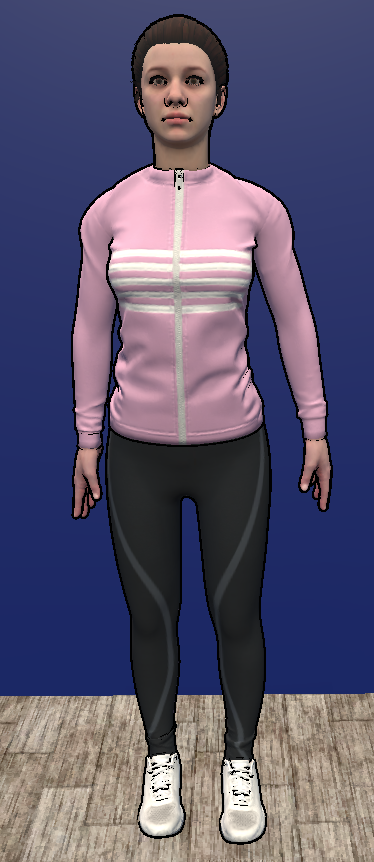
\includegraphics[height=4.70cm,width=0.95\textwidth,keepaspectratio]{Mixamo/Mixamo_vhull.png}\\[0.15em]{\color{kngrey}\tiny Mixamo (Jody)}\end{column}
    \begin{column}{0.313\textwidth}\centering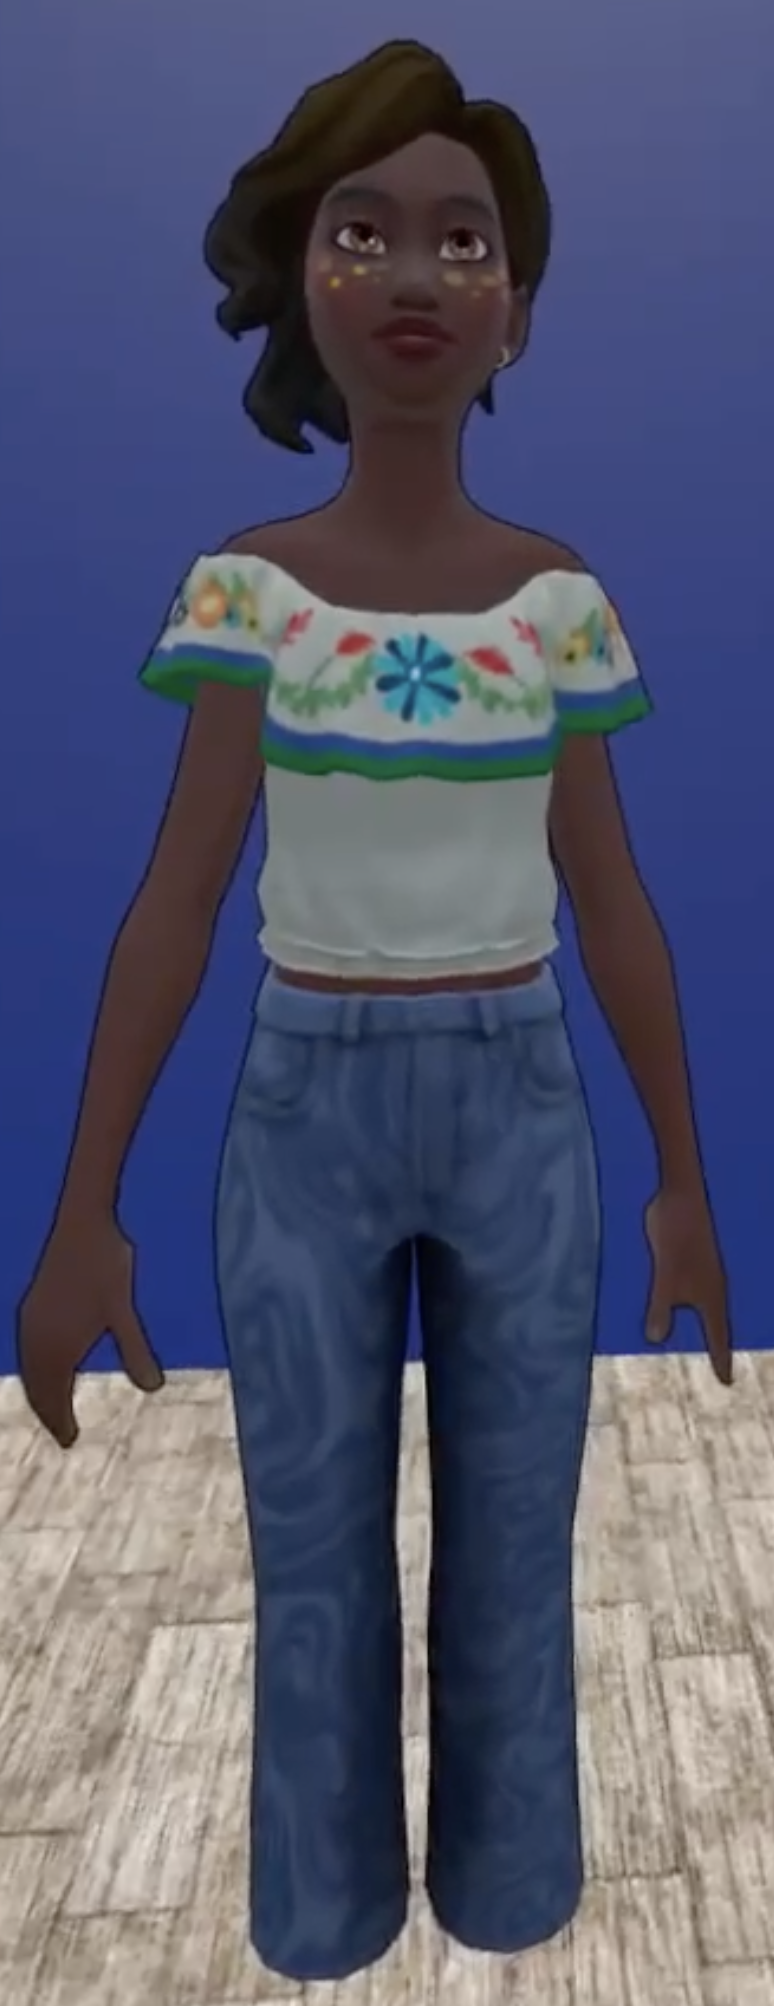
\includegraphics[height=4.70cm,width=0.95\textwidth,keepaspectratio]{Meta/Meta_vhull.png}\\[0.15em]{\color{kngrey}\tiny Meta SDK}\end{column}
    \begin{column}{0.313\textwidth}\centering\includegraphics[height=4.70cm,width=0.95\textwidth,keepaspectratio]{Avaturn/Avaturn_vhull.png}\\[0.15em]{\color{kngrey}\tiny Avaturn}\end{column}
  \end{columns}
\end{frame}

\begin{frame}{Backup — V2 — Toon Shading}{The diffuse term quantised into bands}
  \vspace{0.5em}
  \begin{columns}[c]
    \begin{column}{0.313\textwidth}\centering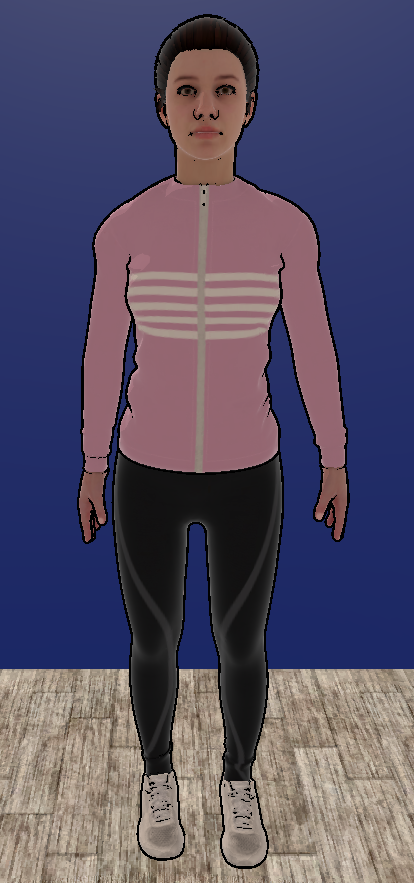
\includegraphics[height=4.70cm,width=0.95\textwidth,keepaspectratio]{Mixamo/Mixamo_v1_toon.png}\\[0.15em]{\color{kngrey}\tiny Mixamo (Jody)}\end{column}
    \begin{column}{0.313\textwidth}\centering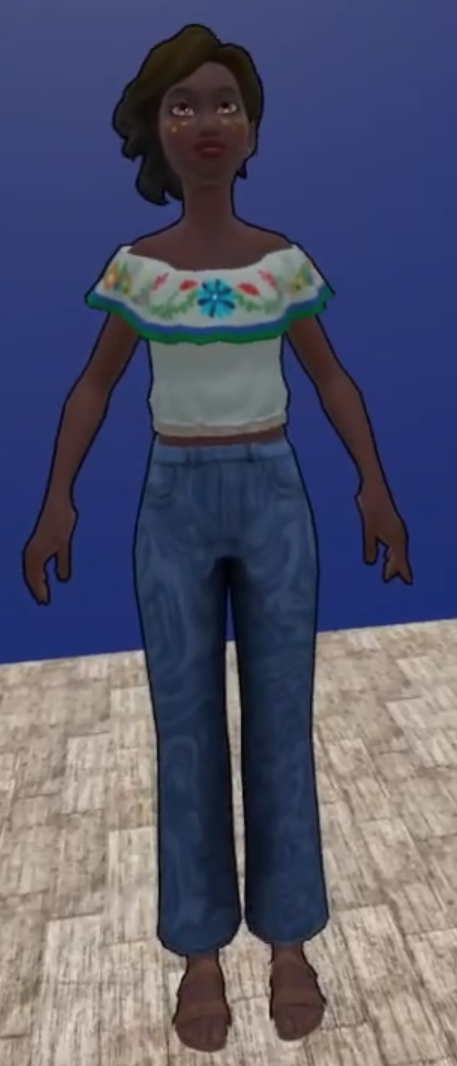
\includegraphics[height=4.70cm,width=0.95\textwidth,keepaspectratio]{Meta/Meta_v1_toon_2.png}\\[0.15em]{\color{kngrey}\tiny Meta SDK}\end{column}
    \begin{column}{0.313\textwidth}\centering\includegraphics[height=4.70cm,width=0.95\textwidth,keepaspectratio]{Avaturn/Avaturn_v1_toon.png}\\[0.15em]{\color{kngrey}\tiny Avaturn}\end{column}
  \end{columns}
\end{frame}

\begin{frame}{Backup — V2.2 — X-Toon Shading}{A 2D ramp: lighting on one axis, abstraction on the other}
  \vspace{0.5em}
  \begin{columns}[c]
    \begin{column}{0.313\textwidth}\centering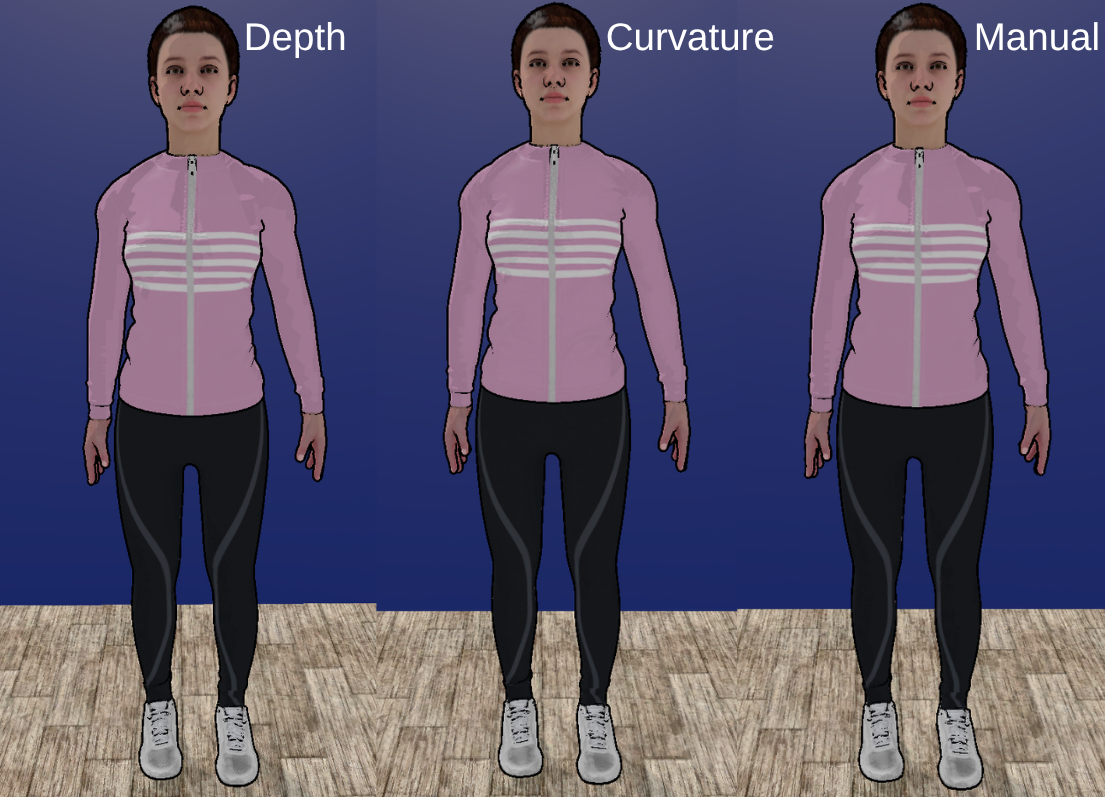
\includegraphics[height=3.30cm,width=0.95\textwidth,keepaspectratio]{Jade/Jody_Xtoon_Comparison.png.png}\\[0.15em]{\color{kngrey}\tiny Mixamo (Jody)}\end{column}
    \begin{column}{0.313\textwidth}\centering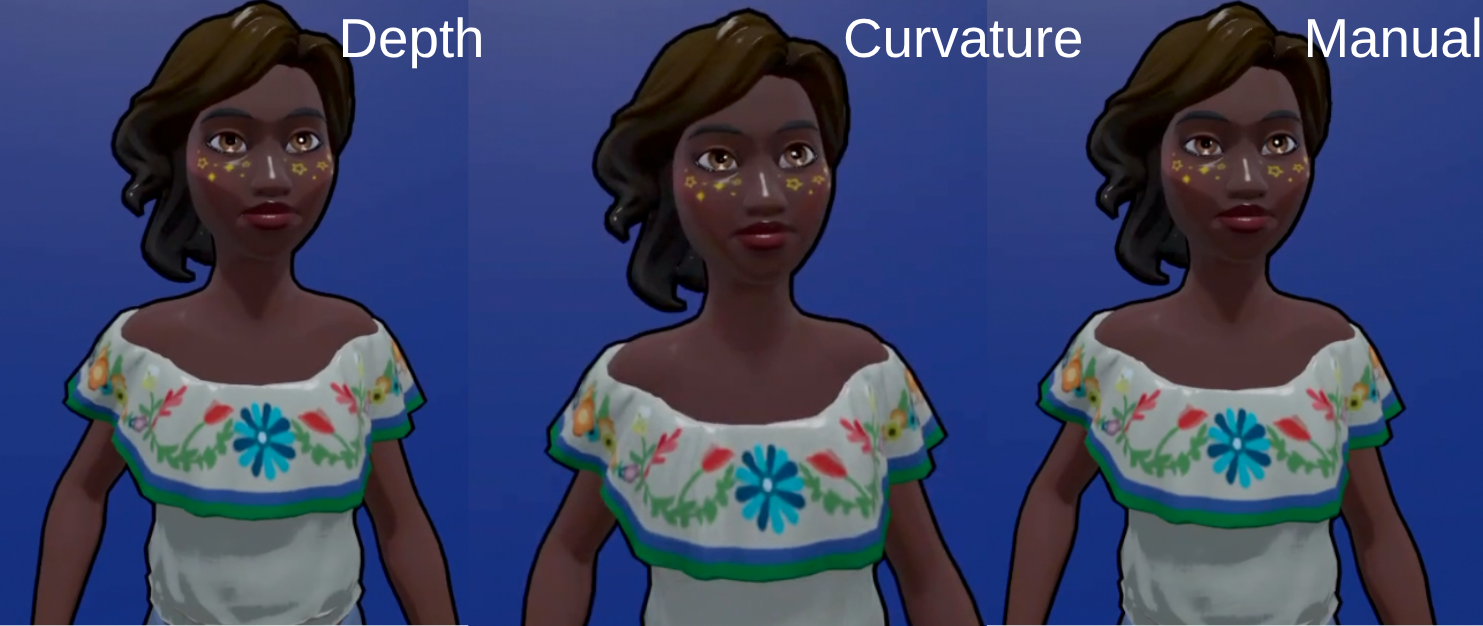
\includegraphics[height=3.30cm,width=0.95\textwidth,keepaspectratio]{mataAvatars/Metavatar_Xtoon_Comparison.png}\\[0.15em]{\color{kngrey}\tiny Meta SDK}\end{column}
    \begin{column}{0.313\textwidth}\centering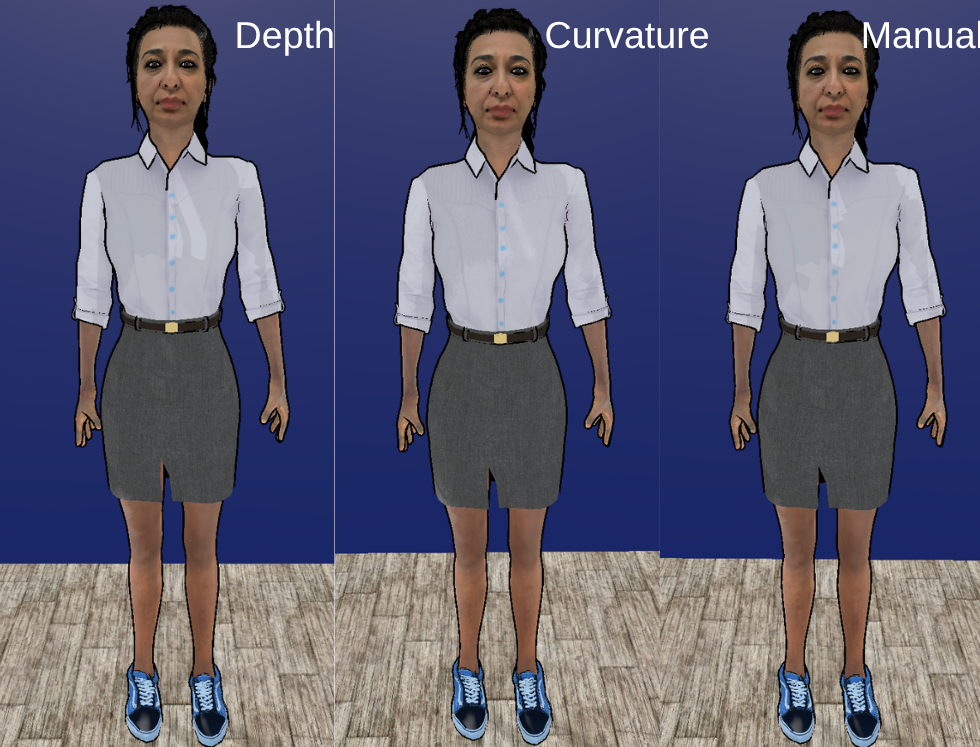
\includegraphics[height=3.30cm,width=0.95\textwidth,keepaspectratio]{Avaturn/Avaturn_Xtoon_Comparison.png.png}\\[0.15em]{\color{kngrey}\tiny Avaturn}\end{column}
  \end{columns}
\end{frame}

\begin{frame}{Backup — V3 — Screen-Space Normal Edge Detection}{Normal derivatives. Creases yes, colour boundaries no}
  \vspace{0.35em}
  \begin{columns}[c]
    \begin{column}{0.48\textwidth}\centering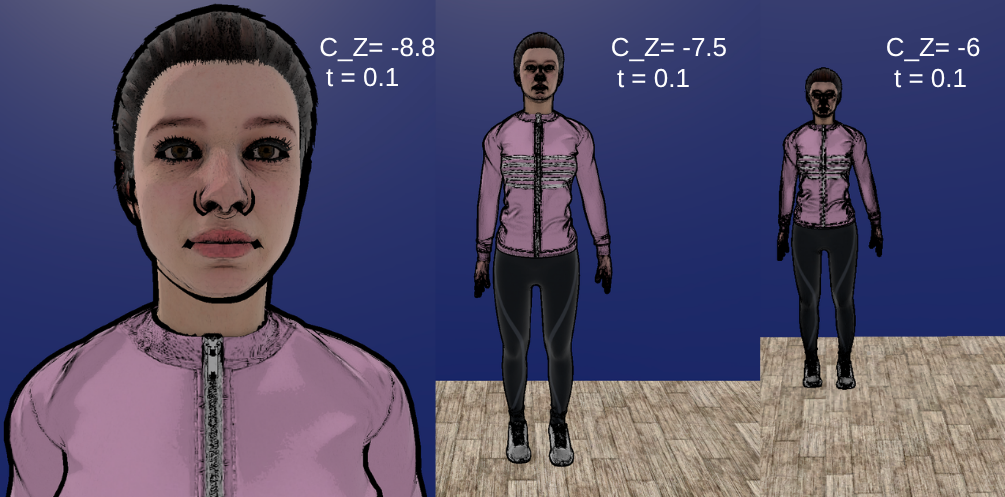
\includegraphics[width=0.66\textwidth]{Jade/Jody_normal.png}\\[0.15em]{\color{kngrey}\tiny Mixamo (Jody)}\end{column}
    \begin{column}{0.48\textwidth}\centering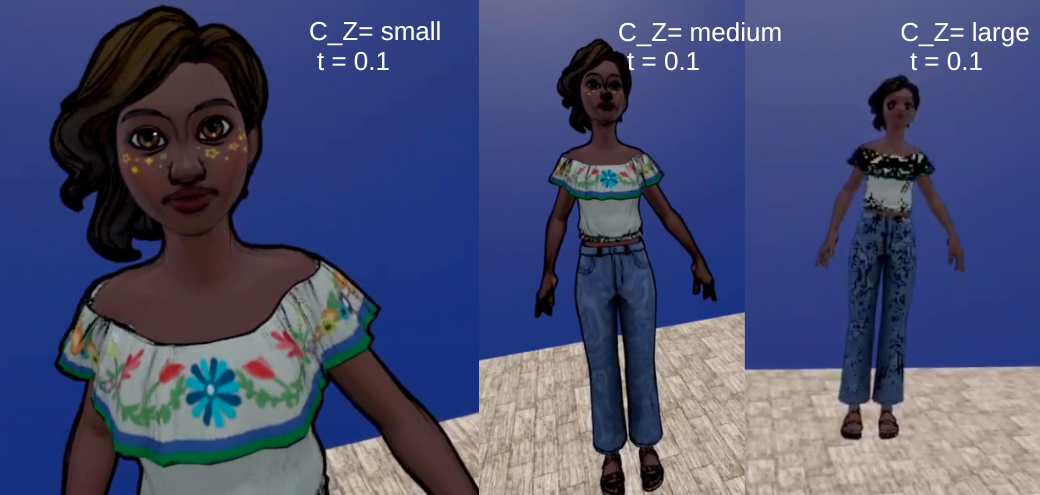
\includegraphics[width=0.66\textwidth]{mataAvatars/metavatar_normal.png}\\[0.15em]{\color{kngrey}\tiny Meta SDK}\end{column}
  \end{columns}
  \vspace{0.4em}
  \begin{columns}[c]
    \begin{column}{0.48\textwidth}\end{column}
    \begin{column}{0.48\textwidth}\centering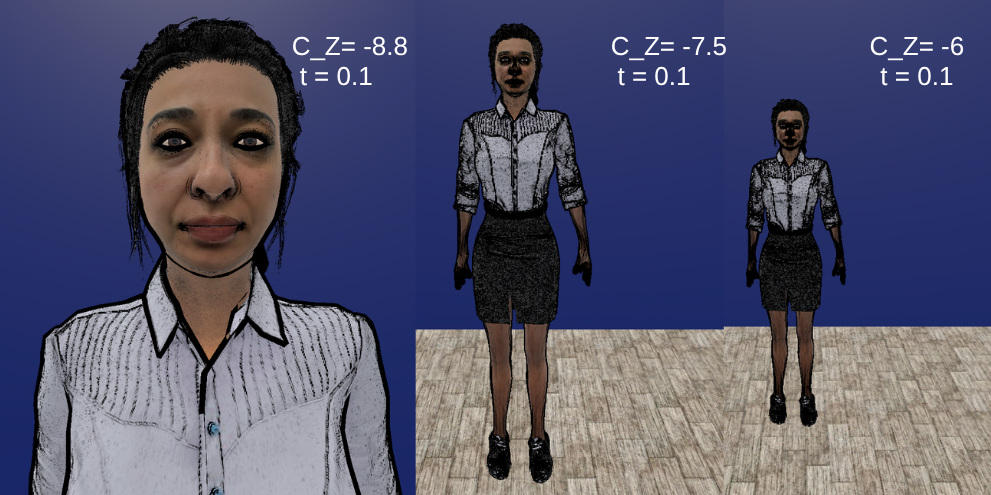
\includegraphics[width=0.66\textwidth]{Avaturn/Avaturn Normal.png}\\[0.15em]{\color{kngrey}\tiny Avaturn}\end{column}
  \end{columns}
\end{frame}

\begin{frame}{Backup — V4 — Sobel Edge Detection}{Gradient on the colour buffer, at rising thresholds}
  \vspace{0.35em}
  \begin{columns}[c]
    \begin{column}{0.48\textwidth}\centering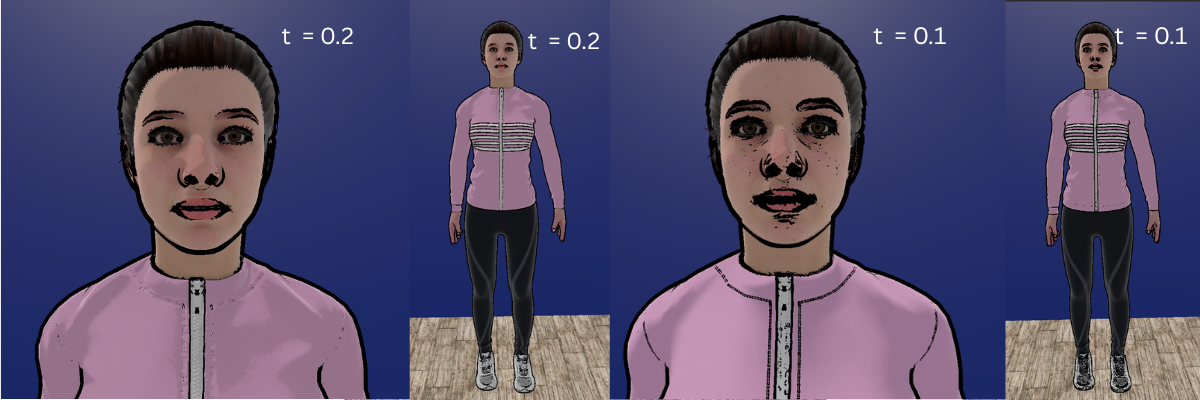
\includegraphics[width=0.96\textwidth]{Jade/jody_sobel.png}\\[0.15em]{\color{kngrey}\tiny Mixamo (Jody)}\end{column}
    \begin{column}{0.48\textwidth}\centering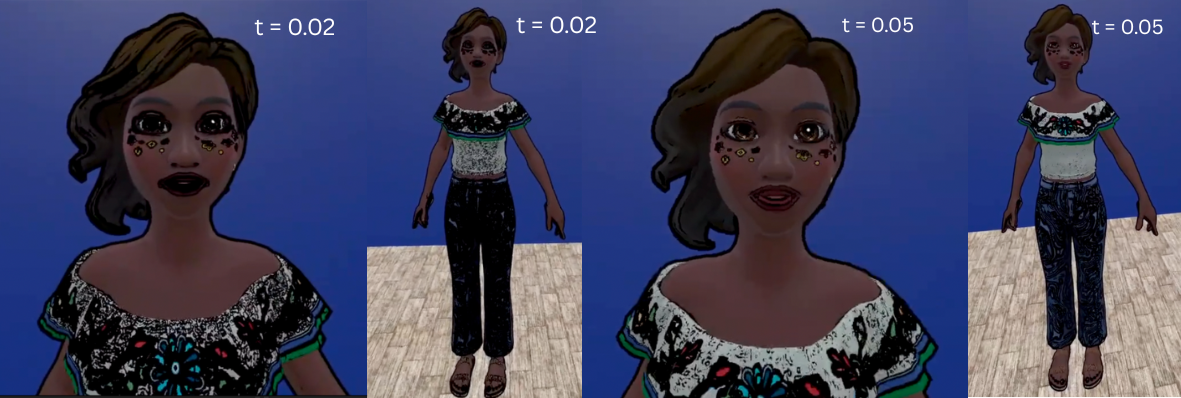
\includegraphics[width=0.96\textwidth]{mataAvatars/metaavatar_sobel.png}\\[0.15em]{\color{kngrey}\tiny Meta SDK}\end{column}
  \end{columns}
  \vspace{0.6em}
  \begin{columns}[c]
    \begin{column}{0.48\textwidth}\end{column}
    \begin{column}{0.48\textwidth}\centering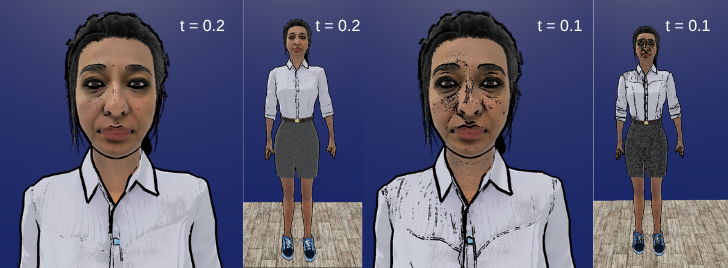
\includegraphics[width=0.96\textwidth]{Avaturn/Avaturn Sobel.png}\\[0.15em]{\color{kngrey}\tiny Avaturn}\end{column}
  \end{columns}
\end{frame}

\begin{frame}{Backup — V4.2 — Gaussian Prefiltered Sobel}{Smoothing before differentiation}
  \vspace{0.35em}
  \begin{columns}[c]
    \begin{column}{0.48\textwidth}\centering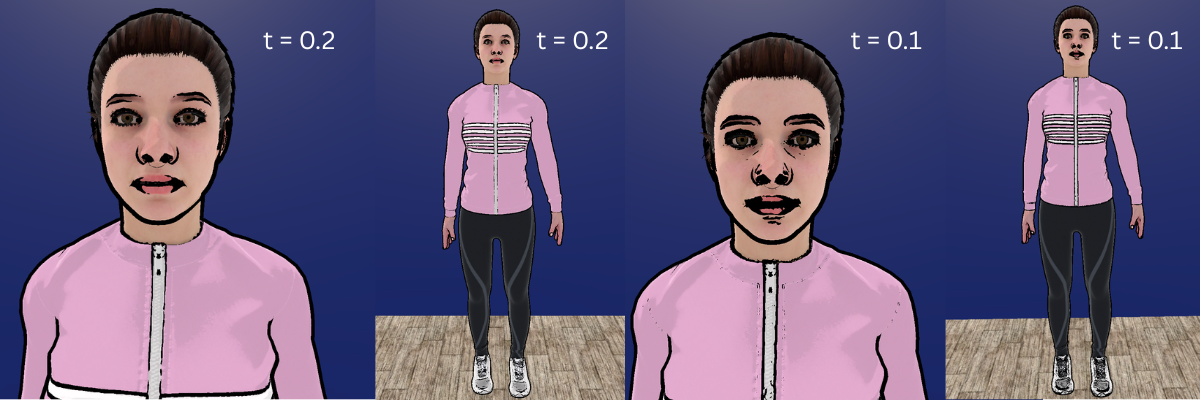
\includegraphics[width=0.96\textwidth]{Jade/Jody_GAussian.png}\\[0.15em]{\color{kngrey}\tiny Mixamo (Jody)}\end{column}
    \begin{column}{0.48\textwidth}\centering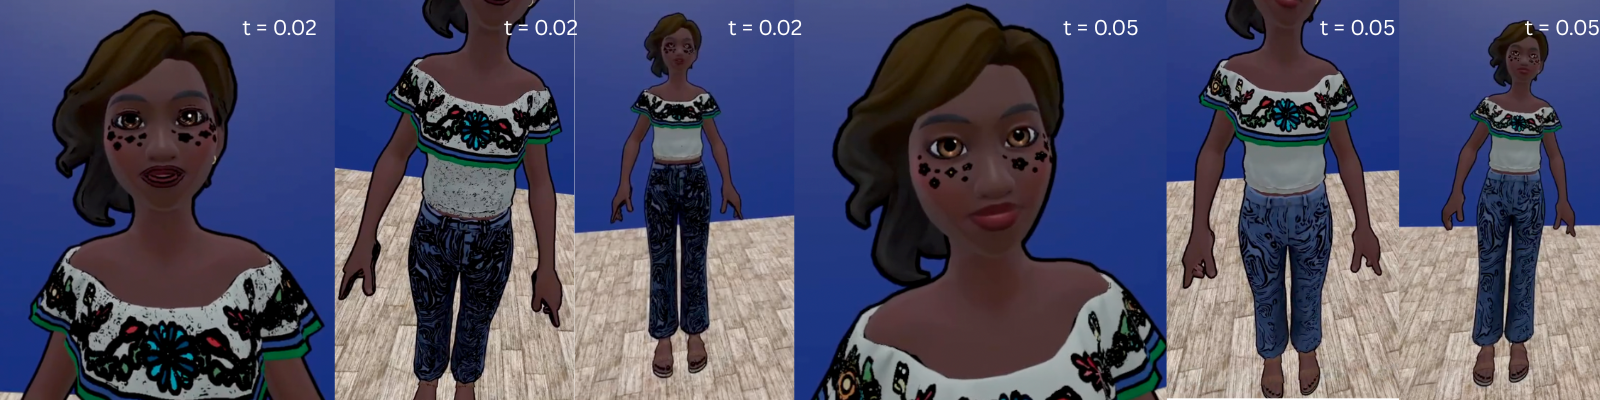
\includegraphics[width=0.96\textwidth]{mataAvatars/metavatar_gaussian.png}\\[0.15em]{\color{kngrey}\tiny Meta SDK}\end{column}
  \end{columns}
  \vspace{0.6em}
  \begin{columns}[c]
    \begin{column}{0.48\textwidth}\end{column}
    \begin{column}{0.48\textwidth}\centering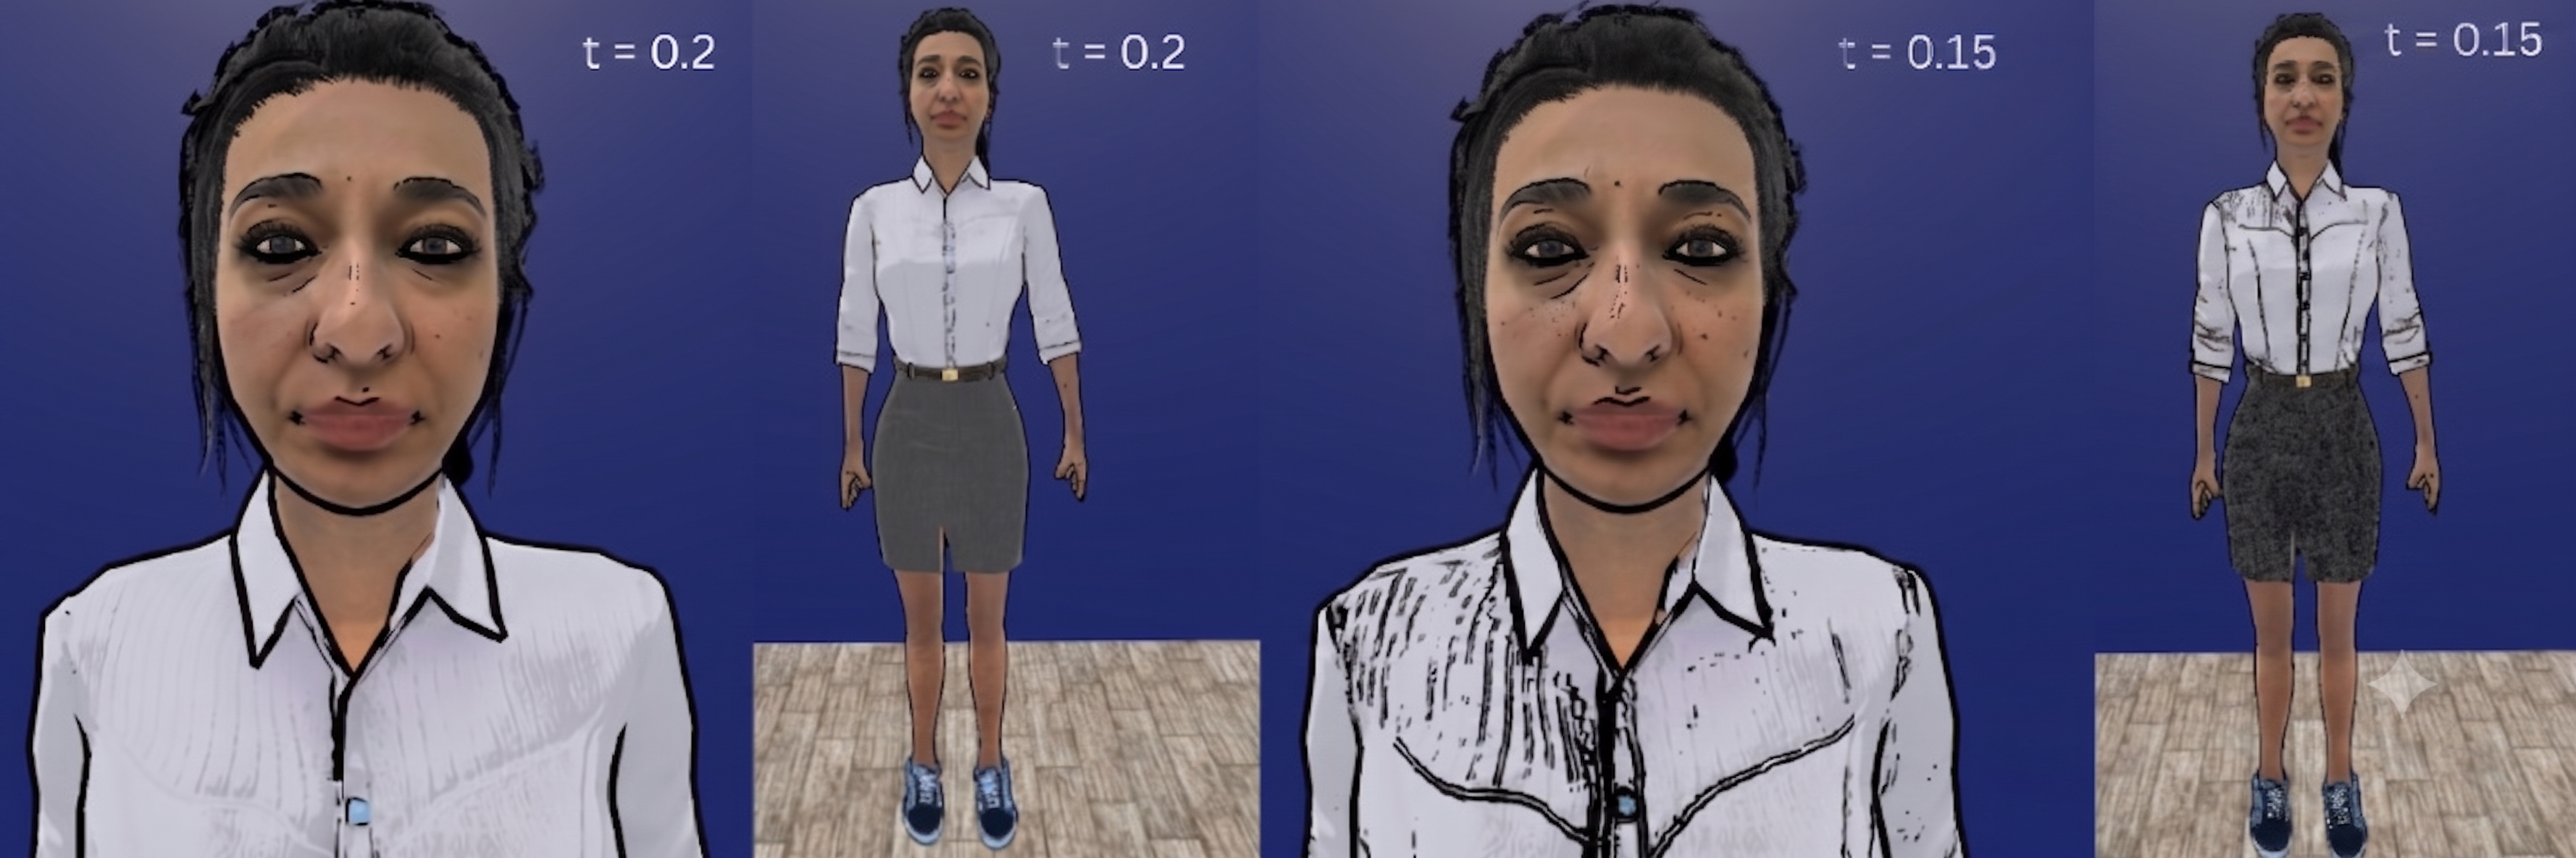
\includegraphics[width=0.96\textwidth]{Avaturn/avaturn_Gaussian.png}\\[0.15em]{\color{kngrey}\tiny Avaturn}\end{column}
  \end{columns}
\end{frame}

\begin{frame}{Backup — V5 — Hierarchical Edge Detection with Multiple Cues}{Depth, normal and colour layers merged}
  \vspace{0.5em}
  \begin{columns}[c]
    \begin{column}{0.313\textwidth}\centering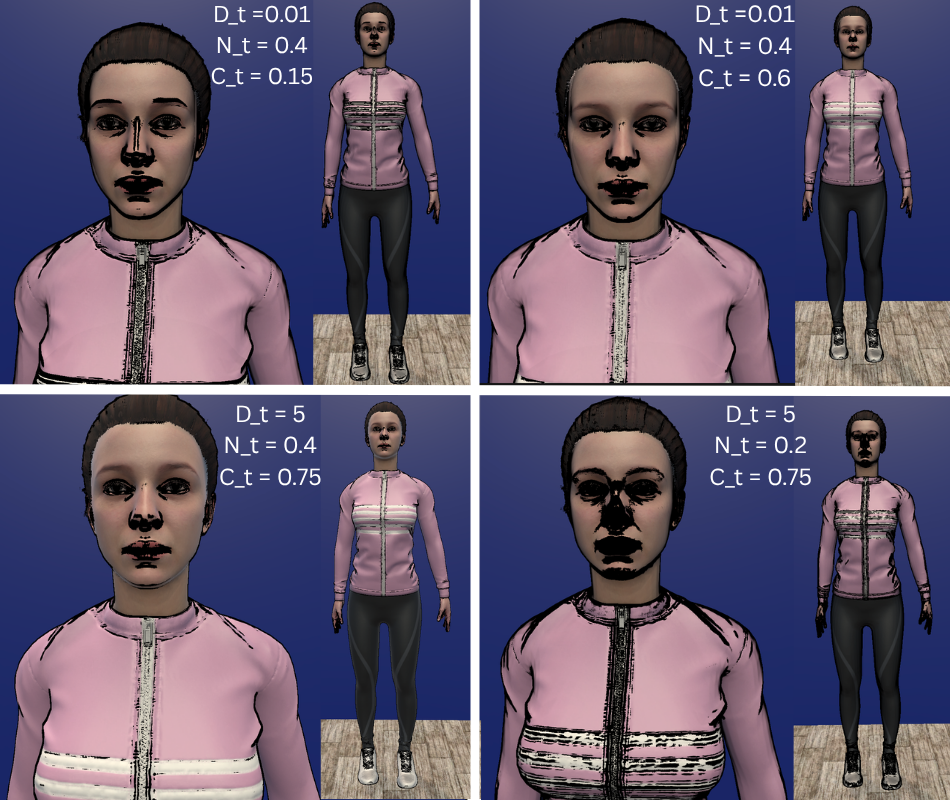
\includegraphics[height=3.60cm,width=0.95\textwidth,keepaspectratio]{Jade/jody_hier_sqr.png}\\[0.15em]{\color{kngrey}\tiny Mixamo (Jody)}\end{column}
    \begin{column}{0.313\textwidth}\centering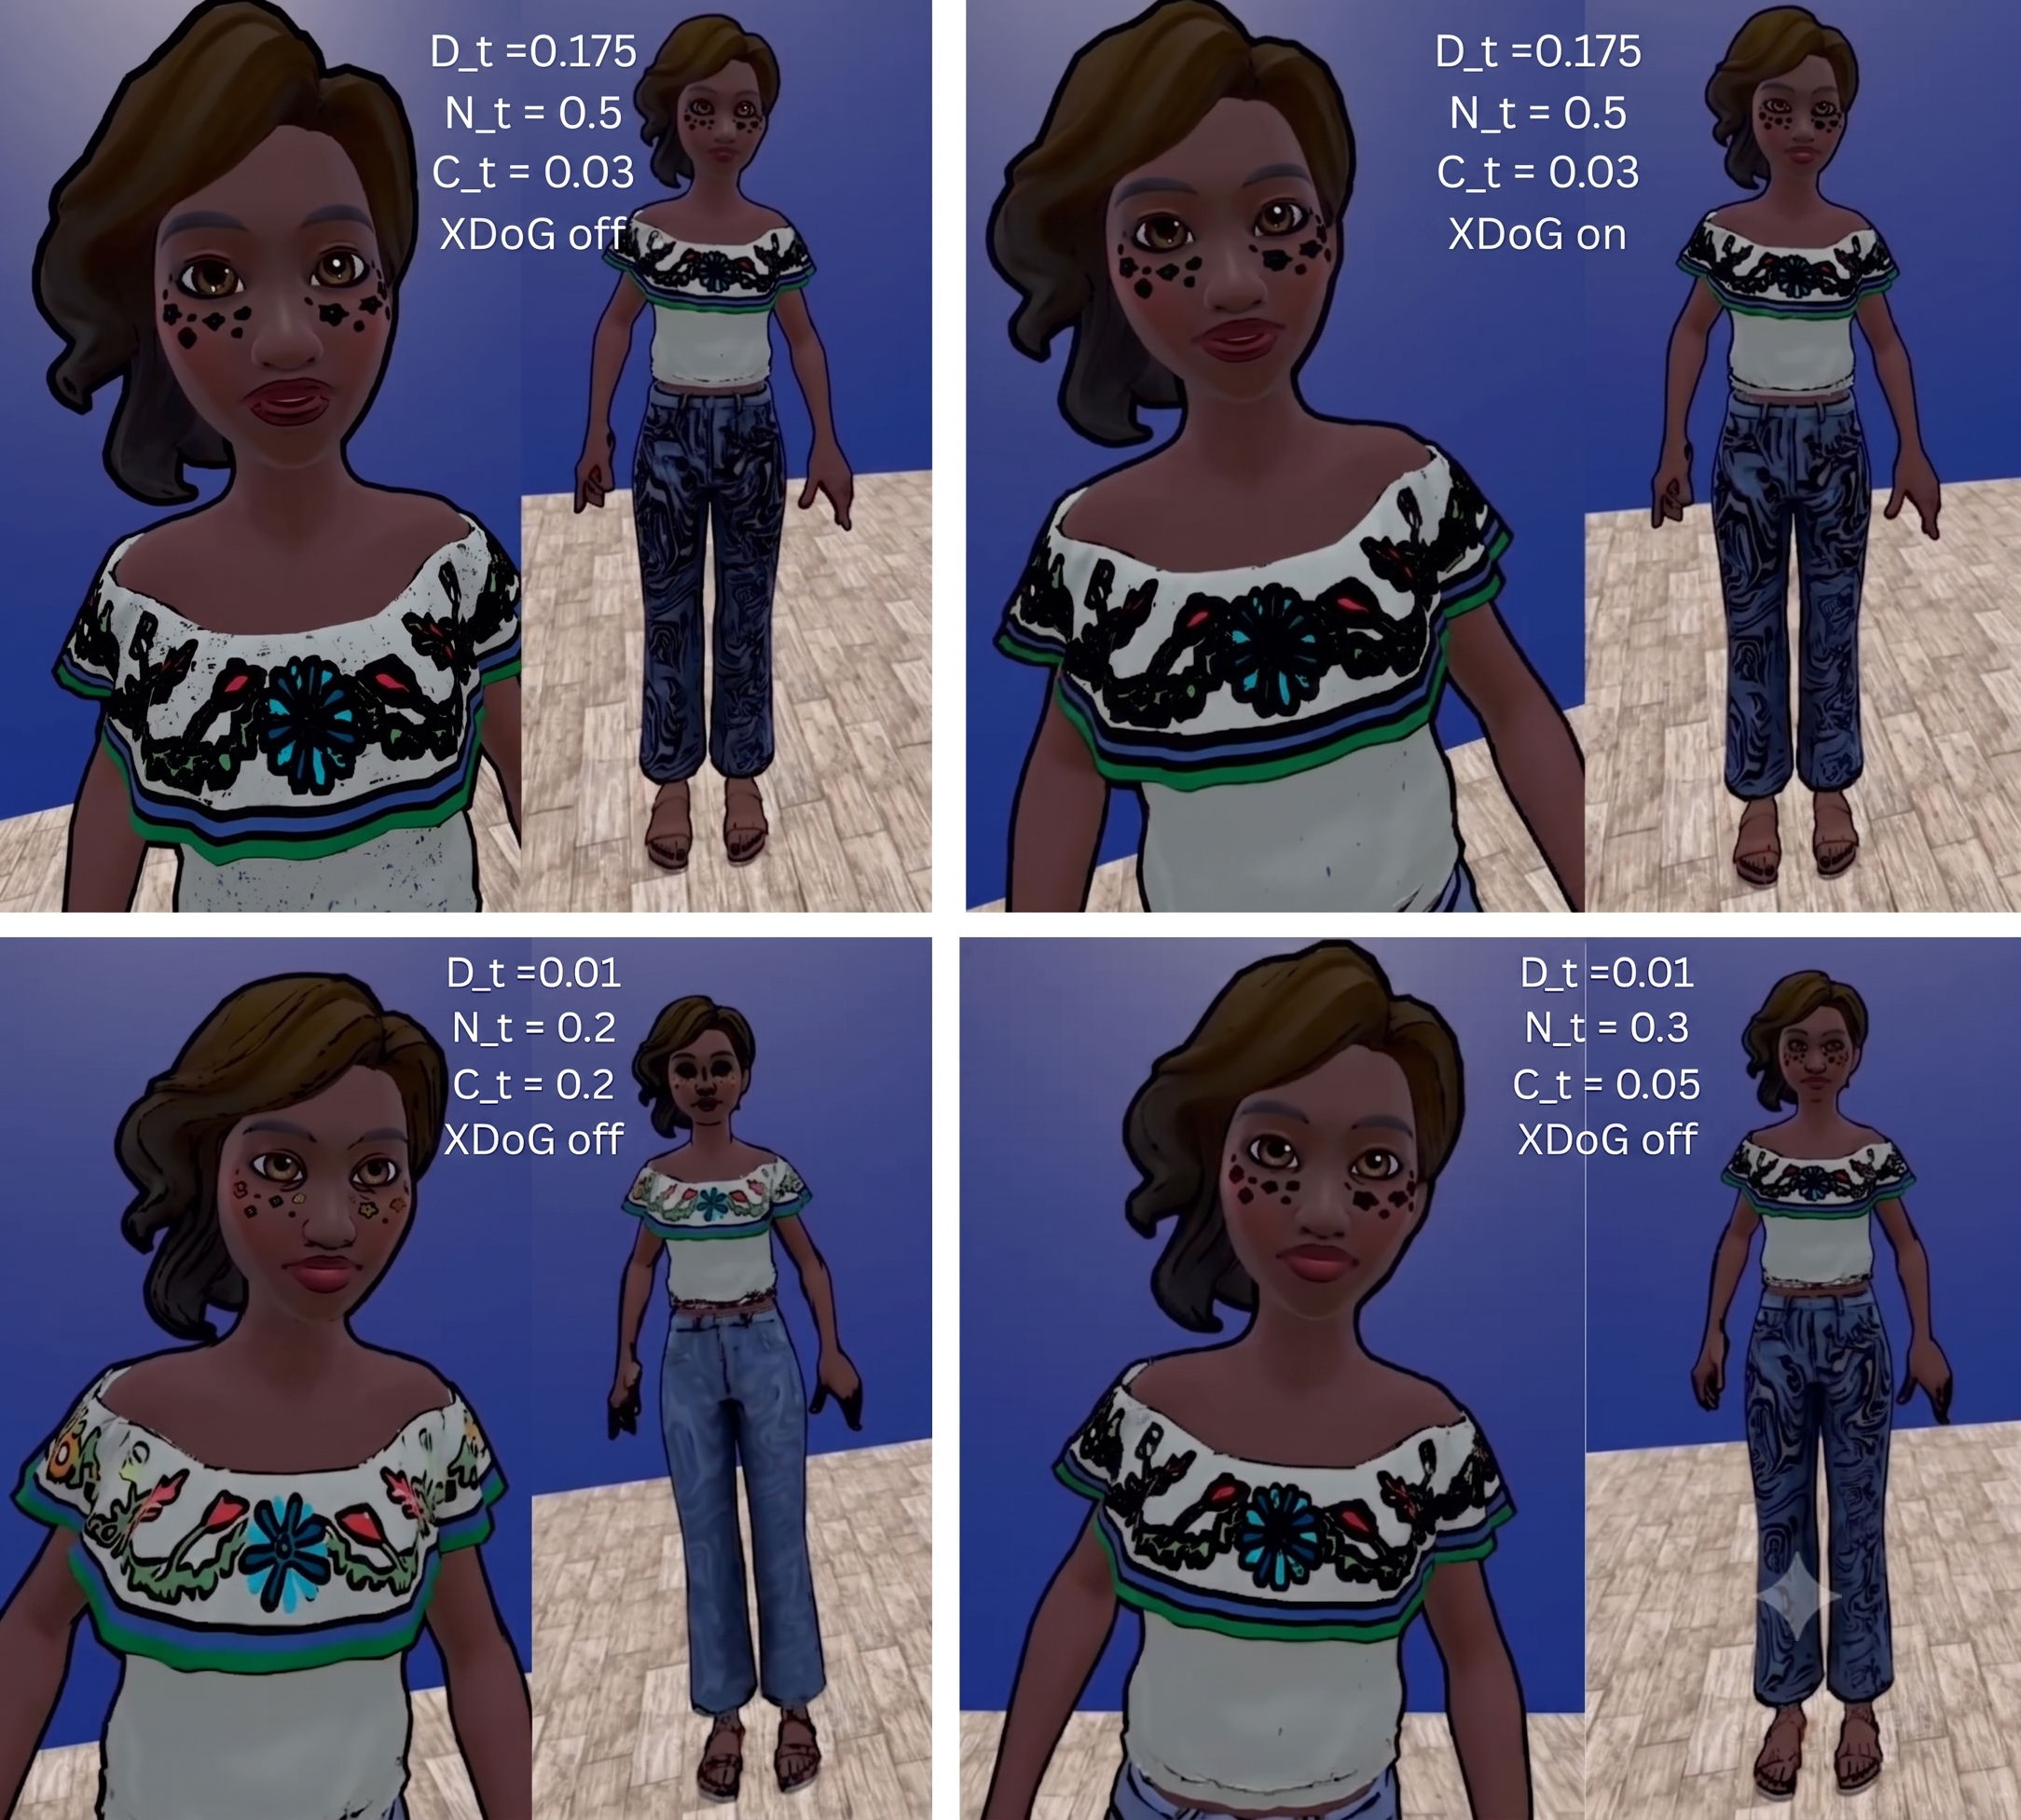
\includegraphics[height=3.60cm,width=0.95\textwidth,keepaspectratio]{mataAvatars/Matavatar_hier_sqr.png}\\[0.15em]{\color{kngrey}\tiny Meta SDK}\end{column}
    \begin{column}{0.313\textwidth}\centering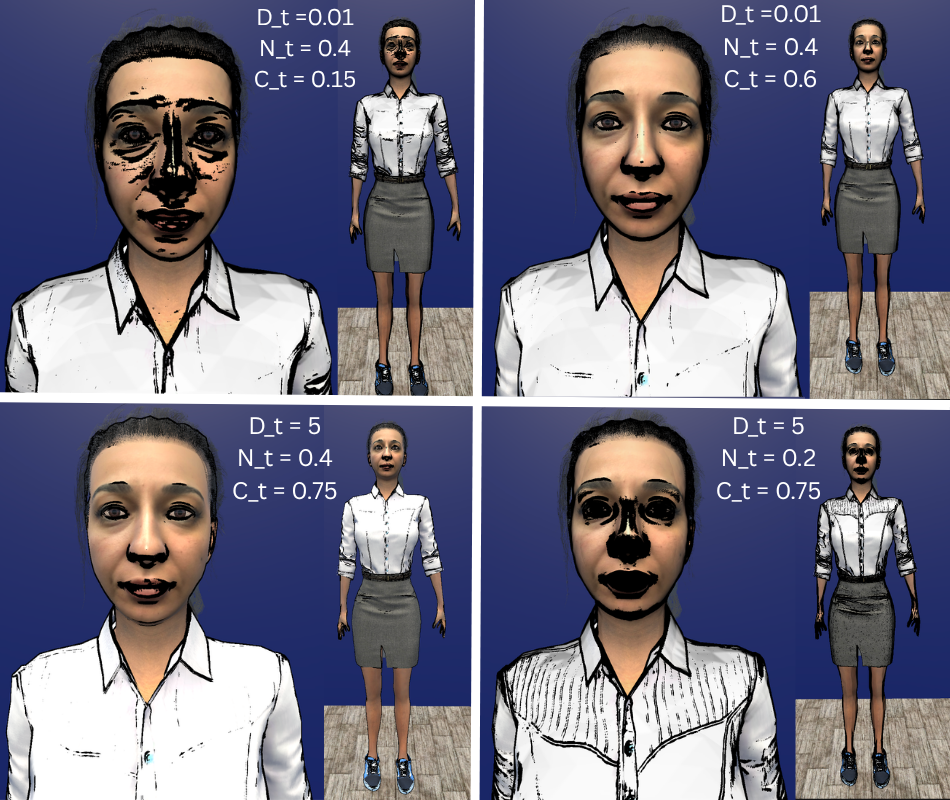
\includegraphics[height=3.60cm,width=0.95\textwidth,keepaspectratio]{Avaturn/avaturn_hier_sqr.png}\\[0.15em]{\color{kngrey}\tiny Avaturn}\end{column}
  \end{columns}
\end{frame}

\begin{frame}{Backup — V6 — Kuwahara Painterly Filter}{Anisotropic painterly filtering of the surface}
  \vspace{0.35em}
  \begin{columns}[c]
    \begin{column}{0.48\textwidth}\centering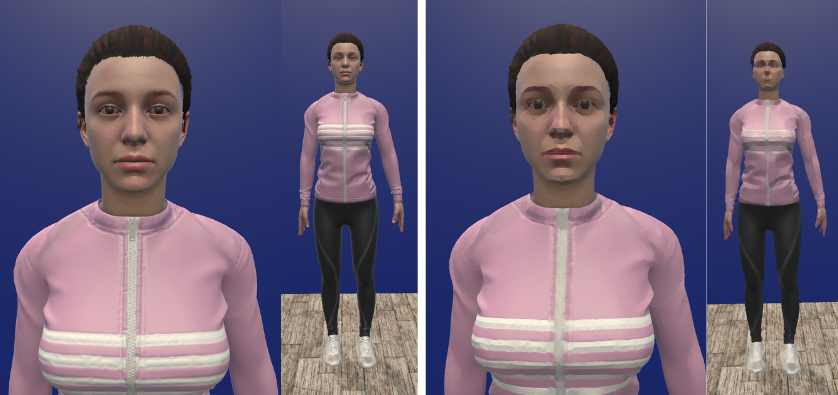
\includegraphics[width=0.90\textwidth]{Mixamo/kuw_mixamo_2.png}\\[0.15em]{\color{kngrey}\tiny Mixamo (Jody)}\end{column}
    \begin{column}{0.48\textwidth}\centering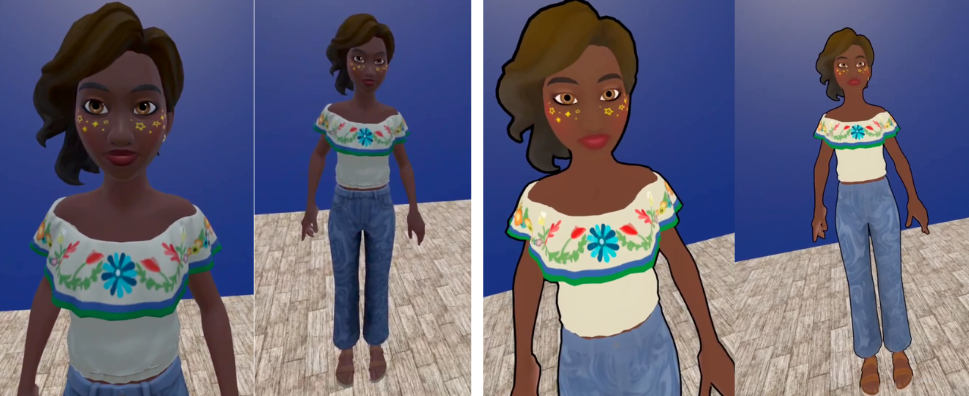
\includegraphics[width=0.90\textwidth]{Meta/Meta_Kuwahara.png}\\[0.15em]{\color{kngrey}\tiny Meta SDK}\end{column}
  \end{columns}
  \vspace{0.6em}
  \begin{columns}[c]
    \begin{column}{0.48\textwidth}\end{column}
    \begin{column}{0.48\textwidth}\centering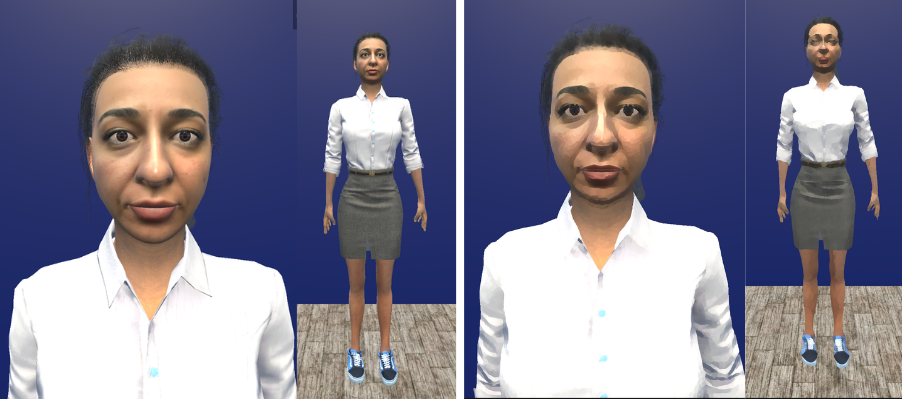
\includegraphics[width=0.90\textwidth]{Avaturn/kuw_avaturn_2.png}\\[0.15em]{\color{kngrey}\tiny Avaturn}\end{column}
  \end{columns}
\end{frame}

\begin{frame}{Backup — V1 and V2 per platform}{Technical review 2/6: built, input and result}
  \vspace{0.1em}
  \techtab{%
    \techhead{V1 Geometric Silhouette Outline}
    Built & Outline pass: front faces culled, vertices pushed out along the normal, $\mathbf{P}'=\mathbf{P}+\mathbf{N}w$, flat colour. Depth \hl{written}, standard test, depth bias against z-fighting & Same displacement and culling. Depth write \bad{disabled}, looser depth test, to avoid clashing with the SDK's depth compositing \\
    Input & Alpha cutout $0.1$ clipped in \hl{both} passes, so hair cards and eyelashes keep their shape & Transparency already \hl{resolved by the SDK}, no manual cutout \\
    Result & \multicolumn{2}{>{\raggedright\arraybackslash}m{0.88\textwidth}}{Same stable silhouette on all three, vertex stage only. Limit: outer contour only, flat planes give no outline} \\
    \rowrule
    \techhead{V2 Toon Shading}
    Built & Lambert $\mathbf{N}\cdot\mathbf{L}$ quantised, $\lfloor s\cdot n\rfloor/n$, \hl{4 bands}, a narrow smoothstep per band edge, shadow strength remap, ambient and rim highlight & \hl{Posterises the lit RGB} per channel, rounding to the nearest band (floor would darken), then a saturation control \\
    Input & The lighting term, before shading & The finished SDK colour, already containing subsurface scattering, hair shading and eye glints \\
    Result & \multicolumn{2}{>{\raggedright\arraybackslash}m{0.88\textwidth}}{Same flat-band look on all three. Limit: bands tied to the lighting, no interior edges} \\
  }
\end{frame}

\begin{frame}{Backup — V2.2 and V3 per platform}{Technical review 3/6: built, input and result}
  \vspace{0.1em}
  \techtab{%
    \techhead{V2.2 X-Toon Shading}
    Built & 2D ramp: U = remapped $\mathbf{N}\cdot\mathbf{L}$, V from \hl{depth, curvature or manual} mode. Abstraction compression flattens bands, shadow colour blend, Blinn-Phong highlight & Same ramp. World position passed in as an \hl{extra argument}, light and shadow fetched per fragment \\
    Input & Normal field abstraction with a \hl{blurred normal map} through the tangent frame. Shadow coordinate per vertex & \bad{No tangent frame} in the hook: geometric smoothing only. Depth mode equals manual, head-and-shoulders depth range too narrow \\
    Result & \multicolumn{2}{>{\raggedright\arraybackslash}m{0.88\textwidth}}{At the 1\,m study framing depth and curvature hardly vary, so \hl{manual mode} was used, detail bias 0.5} \\
    \rowrule
    \techhead{V3 Screen-Space Normal Edge Detection}
    Built & \multicolumn{2}{>{\raggedright\arraybackslash}m{0.88\textwidth}}{Identical everywhere: \texttt{ddx}/\texttt{ddy} of the world normal, magnitude $M_N$, smoothstep around threshold $\tau\pm\sigma$, blended to the line colour} \\
    Input & Normal map decoded and rotated by the tangent frame, \hl{one extra sample} & SDK's composited normal, \hl{no extra sample}, but only interpolated geometric detail \\
    Result & Rich edge network on clothing folds and seams & \bad{Much sparser} interior lines \\
    & \multicolumn{2}{>{\raggedright\arraybackslash}m{0.88\textwidth}}{All three: line width grows with distance, colour boundaries (brows, lips) missed} \\
  }
\end{frame}

\begin{frame}{Backup — V4 and V4.2 per platform}{Technical review 4/6: built, input and result}
  \vspace{0.1em}
  \techtab{%
    \techhead{V4 Sobel Edge Detection}
    Built & 8 neighbour taps at UV offsets, BT.709 luminance, $G_x$, $G_y$, magnitude against \hl{one threshold} & Same gradient, plus a \hl{band gate} (min and max) and \hl{seam rejection} on the luminance range \\
    Input & \hl{Raw albedo}: material boundaries, not lighting & \bad{Composited PBR colour}: shadows, specular and UV seams also respond \\
    Result & Mixamo clean at $t=0.2$. Avaturn: \bad{baked lighting} at the nose bridge, $t=0.3$ removes facial contours. Fixed by texture preprocessing & Lower threshold needed, edges cleaner than Avaturn, less photographic noise in the input \\
    \rowrule
    \techhead{V4.2 Gaussian Prefiltered Sobel}
    Built & \multicolumn{2}{>{\raggedright\arraybackslash}m{0.88\textwidth}}{Shared helper: each of the 8 taps a 9-tap weighted blur, weights normalised, \hl{up to 72 samples}. Band gate replaces the seam gate, four smoothsteps and a power curve sharpen the result} \\
    Controls & Four sharpening steps toggled separately. Presets Light, Moderate, Aggressive (default Light) & One \hl{tightness scalar} drives all four steps \\
    Result & Mixamo: fewer compression artefacts. Avaturn: \bad{baked illumination remains}, presets amplify it & Fewer high-frequency artefacts, cleaner clothing edges \\
  }
\end{frame}

\begin{frame}{Backup — V5 per platform}{Technical review 5/6: hierarchical edges after AHEAD, three cues fused by max-pooling}
  \vspace{0.1em}
  \techtab{%
    Architecture & \hl{URP renderer feature}, a full-screen post-processing pass & \bad{Per-fragment hook}, no extra pass \\
    \rowrule
    Depth layer & Roberts Cross on the \hl{scene depth texture}, linear eye depth, normalised & \texttt{ddx}/\texttt{ddy} of the \hl{distance to the camera}, normalised. Cannot see the background \\
    \rowrule
    Normal layer & Roberts Cross on the scene normal buffer. Replaces AHEAD's gradient structure layer, since baked light would read as geometry & V3 normal derivative plus the \hl{AHEAD dark-area gain}, $\min(1/(3L+0.1),\,4)$ \\
    \rowrule
    Colour layer & Roberts Cross on luminance plus a \hl{chromatic term} for equal-brightness edges & \hl{XDoG}: two blurs subtracted, tanh threshold, cancels broad baked lighting \\
    \rowrule
    Gain and fusion & Brightness-based factor, full on depth and colour, half on normal. Max-pooling & Max-pooling, then one extra smoothstep \\
    \rowrule
    Isolation & \hl{Avatar mask} pass on a dedicated rendering layer & Not needed, the hook only runs on avatar fragments \\
    \rowrule
    Result & Richer interior lines, but \bad{no clear facial segments}, false lines at the nose bridge & \bad{No outer silhouette}, XDoG reduces false responses \\
  }
  \vspace{0.3em}
  {\tiny\color{kngrey}Excluded by the parameter adjustment study, R5, $p<.001$. Mixamo and Avaturn source: \texttt{HierarchicalEdgeDetection.shader}.\par}
\end{frame}

\begin{frame}{Backup — V6 per platform}{Technical review 6/6: anisotropic Kuwahara after Kyprianidis}
  \vspace{0.1em}
  \techtab{%
    Passes & \hl{Three}: (1) structure tensor from a Sobel gradient, (2) 5-tap separable Gaussian blur of the tensor, (3) the filter & \bad{One}, inside the hook \\
    \rowrule
    Tensor & Sobel on luminance, \hl{blurred} before use & \texttt{ddx}/\texttt{ddy} of the lit luminance, \bad{unblurred}, carries lighting too \\
    \rowrule
    Ellipse & Orientation and anisotropy from the eigenvalues, clamped linear blend of the axes & Same eigen decomposition, Kyprianidis ratio formula with an extra eccentricity parameter \\
    \rowrule
    Sampling & Every pixel in the radius sorted into \hl{8 sectors}, cost grows with the radius & Fixed \hl{3 samples per sector} plus one shared, constant cost \\
    \rowrule
    Weight & $1/(1+\sigma^q)$, the 2009 form, variance passed in, exponent halved & $\max(\tau,\sigma)^{-q}$, the thresholded 2011 form \\
    \rowrule
    Composite & Through the avatar mask, as a post-process & Blended by a strength parameter \\
    \rowrule
    Result & Coherent painterly regions, \good{strokes follow} clothing and facial contours & \bad{No coherent regions}, local colour saturation amplified \\
  }
  \vspace{0.3em}
  {\tiny\color{kngrey}All three: the painterly look only appears at a large radius, where brows, lips and irises disappear. Excluded by the parameter adjustment study, R4, $p=.003$.\par}
\end{frame}

\begin{frame}{Backup — Statistical tests: rankings}{People ranked pictures, so the tests work on order only, not on averages}
  \vspace{-0.2em}
  \begin{columns}[T,onlytextwidth]
    \begin{column}{0.325\textwidth}
      \panelheadsm{1. Borda: who wins?}
      \noindent\colorbox{knlight}{\parbox{0.96\textwidth}{\vspace{2pt}\scriptsize\raggedright
        Rank 1 earns the most points, last place 1 point, summed over everyone. A \hl{score}, not a test.\vspace{2pt}}}
    \end{column}
    \begin{column}{0.325\textwidth}
      \panelheadsm{2. Friedman: random or not?}
      \noindent\colorbox{knlight}{\parbox{0.96\textwidth}{\vspace{2pt}\scriptsize\raggedright
        Were some pictures \hl{consistently} ranked higher? If not, people ranked at random.\vspace{2pt}}}
    \end{column}
    \begin{column}{0.325\textwidth}
      \panelheadsm{3. Wilcoxon: \#1 really ahead?}
      \noindent\colorbox{knlight}{\parbox{0.96\textwidth}{\vspace{2pt}\scriptsize\raggedright
        Did most people put the winner \hl{above the runner-up}? If not, the top two are tied.\vspace{2pt}}}
    \end{column}
  \end{columns}
  \vspace{0.45em}

  {\centering\scriptsize\setlength{\tabcolsep}{4pt}\renewcommand{\arraystretch}{1.3}
  \begin{tabular}{@{}>{\raggedright\arraybackslash}m{0.04\textwidth}>{\raggedright\arraybackslash}m{0.19\textwidth}>{\raggedright\arraybackslash}m{0.17\textwidth}>{\raggedright\arraybackslash}m{0.17\textwidth}>{\raggedright\arraybackslash}m{0.15\textwidth}>{\raggedright\arraybackslash}m{0.19\textwidth}@{}}
    \toprule
    & \textbf{What changed} & \textbf{1. Borda winner} & \textbf{2. Friedman} & \textbf{3. Wilcoxon} & \textbf{Decision} \\
    \midrule
    R1 & Sobel inner line threshold & 0.03 (160 vs 149 points) & \good{not random}, $p<.001$ & tie with 0.05, $p=.31$ & \hl{0.05}, by appeal question \\
    R2 & Outline width, depth offset & 0.003, offset on & \good{not random}, $p<.001$ & tie with 0.005, $p=.82$ & \textbf{0.003, on}, Borda winner kept \\
    R3 & Shadow strength, detail bias & 0.5 / 1.0 & \bad{random}, $p=.53$ & --- & \hl{0.0 / 0.5}, by appeal question \\
    R4 & Kuwahara hardness, sharpness & \bad{none} & \good{not random}, $p<.001$ & \good{real win}, $p=.003$ & Kuwahara \bad{dropped} \\
    R5 & Hierarchical depth threshold & \bad{none} & \good{not random}, $p<.001$ & \good{real win}, $p<.001$ & Hierarchical layer \bad{dropped} \\
    \bottomrule
  \end{tabular}\par}
  \vspace{0.3em}
  {\centering\tiny\color{kngrey}45 participants, 40 to 44 valid ballots per round. Tests after Dem\v{s}ar~[24]. One Wilcoxon per round, no correction. Main study: same tests, Holm (slide 26).\par}
\end{frame}

\begin{frame}{Backup — Design compared with Canales}{Canales et al.\ 2024~[7]: what was adopted, and what was changed}
  \vspace{0.1em}
  {\tiny
  \setlength{\tabcolsep}{4pt}\renewcommand{\arraystretch}{1.3}
  \begin{tabular}{@{}>{\raggedright\arraybackslash}m{0.15\textwidth}>{\raggedright\arraybackslash}m{0.38\textwidth}>{\raggedright\arraybackslash}m{0.41\textwidth}@{}}
    \toprule
    & \textbf{Canales et al.\ 2024~[7]} & \textbf{This study} \\
    \midrule
    \good{Adopted} & & \\
    Trust model & Mayer et al.: ability, benevolence, integrity & same \\
    Rating scale & 7-point Likert & same \\
    Behaviour & choose one doctor for a second opinion, and the least preferred & \hl{rank} all three advisors: consult, trustworthy, unsettling \\
    Propensity & 7-item propensity to trust survey & single item: \emph{In general, I tend to trust people I meet for the first time} \\
    \midrule
    \hl{Changed} & & \\
    Medium & immersive VR, Meta Quest 2, interactive interview & prerecorded video in a browser, no interaction \\
    Identity & three doctors, identity crossed with style & \hl{one speaker}, identity held constant \\
    Conditions & caricature, mid, realistic & real video, photorealistic avatar, NPR avatar \\
    Scenario & one medical scenario, kidney lump, second opinion & three everyday decisions: career, travel, learning \\
    Speech & answers to three questions, one per trust dimension & one recommendation, about 22 s \\
    Trust items & 5 ability, 5 benevolence, 6 integrity, 4 overall trust & 3 + 3 + 3, no overall trust items \\
    Order & six identity and style combinations & $3\times3$ Latin square, three versions \\
    Analysis & linear mixed models, exact multinomial test & RM-ANOVA with Holm, TOST, multilevel regression, Friedman and Wilcoxon \\
    Sample & $n=66$ & $n=41$ \\
    \bottomrule
  \end{tabular}\par}
\end{frame}

\begin{frame}{Backup — The three scenarios}{Order held constant, conditions rotated by version}
  \vspace{-0.3em}
  {\centering\scriptsize
  \setlength{\tabcolsep}{4pt}\renewcommand{\arraystretch}{1.12}
  \begin{tabular}{@{}>{\raggedright\arraybackslash}m{0.07\textwidth}>{\raggedright\arraybackslash}m{0.15\textwidth}>{\raggedright\arraybackslash}m{0.33\textwidth}>{\raggedright\arraybackslash}m{0.21\textwidth}>{\raggedright\arraybackslash}m{0.17\textwidth}@{}}
    \toprule
    & \textbf{Scenario} & \textbf{The two options} & \textbf{Advisor picks} & \textbf{Written with in mind} \\
    \midrule
    Video 1 & Career choice    & Job A generalist, lower pay \newline Job B specialist, higher pay      & \hl{Job A}, presented first    & Ability \\
    \rowrule
    Video 2 & Travel route     & Route A direct, 10 min spare \newline Route B one transfer, 40 min spare & \hl{Route B}, presented second  & Benevolence, Ability \\
    \rowrule
    Video 3 & Learning resource & Option A course, EUR 350, certificate \newline Option B free videos, no certificate & \hl{Option A}, presented first & Integrity \\
    \bottomrule
  \end{tabular}\par}
  \vspace{0.6em}

  \begin{columns}[T]
    \begin{column}{0.52\textwidth}
      \panelheadsm{Counterbalancing}
      \noindent\colorbox{knlight}{\parbox{0.96\textwidth}{\vspace{2pt}\scriptsize
      \setlength{\tabcolsep}{4pt}\renewcommand{\arraystretch}{1.25}
      \begin{tabular}{@{}llll@{}}
        \textbf{Version} & \textbf{Video 1} & \textbf{Video 2} & \textbf{Video 3} \\
        A & C2 & C1 & C3 \\
        B & C3 & C2 & C1 \\
        C & C1 & C3 & C2 \\
      \end{tabular}\vspace{2pt}}}
    \end{column}
    \begin{column}{0.44\textwidth}
      \panelheadsm{Design Rules}
      \noindent\colorbox{knlight}{\parbox{0.96\textwidth}{\vspace{2pt}\scriptsize
      \begin{itemize}\setlength{\itemsep}{0.1em}\setlength{\leftmargini}{1.0em}
        \item \hl{Everyday decisions} for a 20 to 35 year old student sample
        \item Equal detail, \hl{one clear cost} per option
        \item Recommendation alternates \hl{A, B, A}, not always presented last
        \item Same \hl{five-step script} every time, see the vignette slides
        \item Baseline recorded \hl{before} the advisor speaks
      \end{itemize}\vspace{2pt}}}
    \end{column}
  \end{columns}
\end{frame}

\begin{frame}{Backup — Vignette 1, Career choice}{Shown on screen before the video}
  \vspace{0.4em}
  \noindent\colorbox{knlight}{\parbox{0.975\textwidth}{\vspace{3pt}\scriptsize
  You recently completed your master's degree and have received two job offers. Both start in one month. You have five days to decide.\\[0.5em]
  \textbf{Job A} is a generalist role at a smaller company. You would define your own work area, your contributions would be directly visible to the team, and the skills you build would transfer across industries. The starting salary is below the industry average for your field.\\[0.5em]
  \textbf{Job B} is a specialist role at a large, well-known company. The employer name carries weight on a CV and the role is in a high-demand field. However, the position involves deep specialisation within a large team, with limited individual visibility. The starting salary is above the industry average for your field.\vspace{3pt}}}
  \vspace{0.8em}

  \panelhead{Advisor, spoken in the video}
  \noindent\colorbox{knpale}{\parbox{0.975\textwidth}{\vspace{3pt}\scriptsize\itshape
  \stp{1}``I'd go with Job A. \stp{2}Yes, the salary is lower right now, \stp{3}but the generalist role gives you a range of experience that is genuinely hard to get later. Salary gaps can be closed in the future. \stp{4}But once you specialise, switching back is costly. \stp{5}Take the pivot while you can.''\vspace{3pt}}}
  \scriptlegend
\end{frame}

\begin{frame}{Backup — Vignette 2, Travel route}{Shown on screen before the video}
  \vspace{0.4em}
  \noindent\colorbox{knlight}{\parbox{0.975\textwidth}{\vspace{3pt}\scriptsize
  You have just arrived by train in a city you have never visited. You need to reach your hotel, where colleagues are expecting you in one hour.\\[0.5em]
  \textbf{Route A} is a direct route on a single line with no transfers. It is straightforward to navigate in an unfamiliar city. If the journey runs on time, you would arrive approximately 10 minutes before your meeting begins.\\[0.5em]
  \textbf{Route B} involves one transfer at a mid-size station you have not used before. If the connection runs on time, you would arrive approximately 40 minutes before your meeting begins. However, the transfer station is unfamiliar and a missed connection could leave you with very little time.\vspace{3pt}}}
  \vspace{0.8em}

  \panelhead{Advisor, spoken in the video}
  \noindent\colorbox{knpale}{\parbox{0.975\textwidth}{\vspace{3pt}\scriptsize\itshape
  \stp{1}``I'd take Route B. \stp{2}Yes, it has a transfer at a station you have never used. \stp{3}But it gets you there forty minutes early. If something goes wrong, you still have enough time to recover. \stp{4}Route A is direct but leaves only ten minutes. That may not be enough. \stp{5}Take the buffer.''\vspace{3pt}}}
  \scriptlegend
\end{frame}

\begin{frame}{Backup — Vignette 3, Learning resource}{Shown on screen before the video}
  \vspace{0.4em}
  \noindent\colorbox{knlight}{\parbox{0.975\textwidth}{\vspace{3pt}\scriptsize
  You want to develop a professional skill that would strengthen your CV and improve your career prospects. You have a few weeks available and you are a student with a limited budget.\\[0.5em]
  \textbf{Option A} is a structured online course from a well-known learning platform. It follows a clear curriculum and awards a recognised certificate you can add to your CV. It costs EUR 350.\\[0.5em]
  \textbf{Option B} is a video tutorial series by a practitioner with a strong reputation. It covers the same material at no cost and you set your own pace. However, there is no certificate and no structured curriculum.\vspace{3pt}}}
  \vspace{0.8em}

  \panelhead{Advisor, spoken in the video}
  \noindent\colorbox{knpale}{\parbox{0.975\textwidth}{\vspace{3pt}\scriptsize\itshape
  \stp{1}``I would take Option A. \stp{2}Yes, 350 euros is a real cost. \stp{3}But the certificate is what matters here. It is not just about what you learn, it is about what you can show. \stp{4}A recruiter cannot verify a free tutorial series. \stp{5}That is worth it.''\vspace{3pt}}}
  \scriptlegend
\end{frame}

\begin{frame}{Backup — Hypotheses and their tests}{Each prediction follows a prior finding}
  \vspace{0.1em}
  {\tiny
  \setlength{\tabcolsep}{4pt}\renewcommand{\arraystretch}{1.45}
  \begin{tabular}{@{}>{\raggedright\arraybackslash}m{0.25\textwidth}>{\raggedright\arraybackslash}m{0.27\textwidth}>{\raggedright\arraybackslash}m{0.21\textwidth}>{\raggedright\arraybackslash}m{0.21\textwidth}@{}}
    \toprule
    \textbf{Hypothesis} & \textbf{Grounded in} & \textbf{Test} & \textbf{Why this test} \\
    \midrule
    H1: C3 less eerie than C2 & Dubosc 2025~[8]: stylised avatars rated less eerie & RM-ANOVA, Holm pairwise & one subscale, three related conditions \\
    H2: C3 no lower trust than C2 & Canales 2024~[7]: style did not lower self-reported trust & pairwise + TOST, $d=0.3$ & a null needs an equivalence test \\
    H3: eeriness lowers, likeability raises trust & Ho 2010~[3]: eeriness distinct from dislike; Alipour 2026~[21]: link not uniform & person-centred multilevel regression & separates within-person change from general trustingness \\
    H4: C3 no lower trust than C1 & Gao 2025~[9]: real speaker above the stylised agent & pairwise + TOST, $d=0.3$ & same as H2, against the real speaker \\
    \bottomrule
  \end{tabular}\par}
  \vspace{0.5em}
  {\scriptsize\color{knblue}H2 and H4 predict \emph{no difference}. A non-significant $p$ is not evidence of equality, so both carry a TOST.\par}
\end{frame}

\begin{frame}{Backup — The rating instruments, and why each}{Canales~[7] supplied the trust battery only, so the remaining scales come from elsewhere}
  \vspace{0.2em}
  {\scriptsize
  \setlength{\tabcolsep}{4pt}\renewcommand{\arraystretch}{1.25}
  \begin{tabular}{@{}>{\raggedright\arraybackslash}m{0.16\textwidth}>{\raggedright\arraybackslash}m{0.22\textwidth}>{\raggedright\arraybackslash}m{0.13\textwidth}>{\raggedright\arraybackslash}m{0.40\textwidth}@{}}
    \toprule
    \textbf{Part} & \textbf{Source} & \textbf{Format} & \textbf{Why this one} \\
    \midrule
    B \ Likeability & \hl{Godspeed}, Bartneck et al.\ 2009~[14] & 5 items, semantic differential 1--5 & Canales measured no likeability. Zell~[15] shows appeal moves with material while realism does not \\
    D \ Eeriness & Ho \& MacDorman 2010~[3] & 8 items, semantic differential 1--5 & Built to separate \hl{eeriness from human likeness}, which the Godspeed indices confound. H1 needs that \\
    E--G \ Trust & Mayer et al.\ 1995~[6], wording after Canales~[7] & 3+3+3, Likert 1--7 & Three separable dimensions, so no single trust score is ever reported \\
    H \ Stylisation & own item & 1 item, Likert 1--7 & Manipulation check: verifies the difference was \hl{seen}, so a null is not an unnoticed manipulation \\
    \bottomrule
  \end{tabular}\par}
  \vspace{0.45em}
  \begin{columns}[T]
    \begin{column}{0.32\textwidth}
      \panelheadsm{Why Godspeed, not an ad hoc scale}
      \panel{%
        \item Published reliability and validity, and widely reused, so results stay comparable
        \item One response format shared by B and D}
    \end{column}
    \begin{column}{0.32\textwidth}
      \panelheadsm{Why no human-likeness scale}
      \panel{%
        \item Godspeed's anthropomorphism subscale was \bad{dropped} before the study ran, and it \bad{confounds} with the eeriness items
        \item Human likeness is a \hl{concept} here, never a measured variable}
    \end{column}
    \begin{column}{0.32\textwidth}
      \panelheadsm{What the form calls them}
      \panel{%
        \item Titles are \hl{neutral} so nobody is primed by a construct name
        \item \emph{Warmth and Appeal} $=$ B, \emph{Impression} $=$ D, \emph{Trust} $=$ E--G, \emph{Overall Impressions} $=$ rankings}
    \end{column}
  \end{columns}
\end{frame}

\begin{frame}{Backup — Trust items: Ability and Benevolence}{Canales et al.\ 2024~[7] next to this study, word for word}
  \vspace{0.1em}
  {\tiny
  \setlength{\tabcolsep}{4pt}\renewcommand{\arraystretch}{1.35}
  \begin{tabular}{@{}>{\raggedright\arraybackslash}m{0.31\textwidth}>{\raggedright\arraybackslash}m{0.36\textwidth}>{\raggedright\arraybackslash}m{0.27\textwidth}@{}}
    \toprule
    \textbf{This study} & \textbf{Closest Canales et al.\ 2024 item} & \textbf{What changed} \\
    \midrule
    \multicolumn{3}{@{}l}{\textbf{\color{knblue}Ability}} \\
    This advisor is capable and competent. & A1: The doctor is very capable of performing his/her job. & doctor $\to$ advisor, no job reference, \emph{competent} added \\
    This advisor seems knowledgeable. & A2: The doctor has much knowledge about the work that needs done. & shortened, no task reference \\
    This advisor seems to have the expertise needed to give sound advice on this kind of decision. & A4: The doctor has specialized capabilities that can increase performance. \newline A5: The doctor is well qualified. & tied to the advice decision, not medical performance \\
    \midrule
    \multicolumn{3}{@{}l}{\textbf{\color{knblue}Benevolence}} \\
    This advisor will act in a benevolent (well meaning) manner. & Pretest prompt: This person will behave in a benevolent (well meaning) manner. & \emph{behave} $\to$ \emph{act} \\
    This advisor would act in my best interest. & B4: The doctor really looks out for what is important to me. & rephrased after the benevolence definition, \emph{best interest of the trustor} \\
    This advisor appears to have good intentions. & B1: The doctor is very concerned about my welfare. & \bad{no direct counterpart}, closest item shown \\
    \bottomrule
  \end{tabular}\par}
  \vspace{0.3em}
  {\tiny\color{kngrey}Canales items from their Supplement 11.1 (post-doctor surveys). Pretest prompts from their Section 3.2, used to rate the doctors' dialogue.\par}
\end{frame}

\begin{frame}{Backup — Trust items: Integrity}{And what was left out of Canales et al.\ 2024~[7]}
  \vspace{0.1em}
  {\tiny
  \setlength{\tabcolsep}{4pt}\renewcommand{\arraystretch}{1.35}
  \begin{tabular}{@{}>{\raggedright\arraybackslash}m{0.31\textwidth}>{\raggedright\arraybackslash}m{0.36\textwidth}>{\raggedright\arraybackslash}m{0.27\textwidth}@{}}
    \toprule
    \textbf{This study} & \textbf{Closest Canales et al.\ 2024 item} & \textbf{What changed} \\
    \midrule
    \multicolumn{3}{@{}l}{\textbf{\color{knblue}Integrity}} \\
    This advisor adheres to a set of principles that I find acceptable. & Pretest prompt: The person adheres to a set of principles that I find acceptable. \newline I6: Sound principles seem to guide the doctor's behavior. & subject only \\
    This advisor appears to be honest. & \bad{no direct counterpart} & --- \\
    This advisor seems sincere. & \bad{no direct counterpart} & --- \\
    \bottomrule
  \end{tabular}\par}
  \vspace{0.6em}
  \begin{columns}[T,onlytextwidth]
    \begin{column}{0.485\textwidth}
      \panelhead{Not Carried Over}
      \panel{%
        \item A3: I feel very confident about the doctor's skills
        \item B2, B3, B5: needs and desires, not hurt me, go out of his/her way
        \item I2 to I5: sense of justice, stick to word, fair dealings, values
        \item All four \hl{overall trust} items, two of them reverse scored
        \item I1 is \bad{blank} in the published supplement}
    \end{column}
    \begin{column}{0.485\textwidth}
      \panelhead{Kept the Same}
      \panel{%
        \item Mayer et al.\ 1995~[6]: ability, benevolence, integrity
        \item 7-point Likert, agree to disagree
        \item Rated once per advisor, after each advisor
        \item Three dimensions analysed separately}
    \end{column}
  \end{columns}
\end{frame}

\begin{frame}{Backup — Composite reliability}{Chapter 6.2.3 — Cronbach's $\alpha$ per subscale}
  \vspace{0.6em}
  \begin{columns}[T]
    \begin{column}{0.46\textwidth}
      \centering
      \begin{tabular}{@{}lcc@{}}
        \toprule
        \textbf{Subscale} & \textbf{Items $k$} & \textbf{$\alpha$} \\
        \midrule
        Likeability & 5 & $.94$ \\
        Eeriness    & 8 & $.87$ \\
        Ability     & 3 & $.96$ \\
        Benevolence & 3 & $.95$ \\
        Integrity   & 3 & $.92$ \\
        \bottomrule
      \end{tabular}
    \end{column}
    \begin{column}{0.50\textwidth}
      \small
      Every subscale clears the conventional $.70$ threshold, and each one was recomputed separately within C1, C2 and C3 rather than on the pooled data alone. All five held in every condition.
      \vspace{0.6em}

      Averaging the items of each subscale into a single composite is therefore justified, and every test reported in this talk runs on those five composites.
    \end{column}
  \end{columns}
\end{frame}

\begin{frame}{Backup — Statistical analysis, step by step}{The order in which the main study was analysed, $n=41$}
  \vspace{-0.4em}
  {\scriptsize\setlength{\tabcolsep}{3pt}\renewcommand{\arraystretch}{1.05}
  \begin{tabular}{@{}>{\raggedright\arraybackslash}m{0.03\textwidth}>{\raggedright\arraybackslash}m{0.25\textwidth}>{\raggedright\arraybackslash}m{0.31\textwidth}>{\raggedright\arraybackslash}m{0.37\textwidth}@{}}
    \toprule
    & \textbf{Method} & \textbf{Question it answers} & \textbf{Result here} \\
    \midrule
    1 & \hl{Cronbach's $\alpha$}, overall and per condition & Do the items of one subscale measure one thing? Minimum $.70$~[3,14] & $.87$ to $.96$ overall, never below $.80$ per condition. Composites formed \\
    \rowrule
    2 & \hl{One-way RM-ANOVA}, one per subscale & Does condition change the rating at all? Same people in all three & All five subscales significant, $p<.001$ \\
    \rowrule
    3 & \hl{Mauchly}, \hl{Greenhouse-Geisser} & Do the pairwise differences vary about equally? Correct the test if not & Correction applied where violated, e.g.\ stylisation question, $W=.53$ \\
    \rowrule
    4 & \hl{Holm} pairwise, $\eta^2_p$, Hedges' $g$ & Which pairs differ, and by how much? & C1 differs from both avatars on all five. \bad{C2 vs C3 on none} \\
    \rowrule
    5 & \hl{TOST}, $d=0.3$~[23] & Are two conditions practically equal? H2, H4 & H2 inconclusive, $p=.240$. H4 not equivalent, $p=.998$ \\
    \rowrule
    6 & \hl{Person-centred multilevel} regression & Within a person, do eeriness and likeability predict trust? H3 & All slopes $p<.001$, in the predicted directions \\
    \rowrule
    7 & \hl{Friedman}, Holm \hl{Wilcoxon} & Do the three rankings differ from chance? Which pairs? & C1 first on consulting and trust. C2 and C3 tied \\
    \rowrule
    8 & ANOVA on \hl{position} and \hl{study version} & Did the order of the videos matter? & Position: no effect. Version: likeability and eeriness \\
    \bottomrule
  \end{tabular}\par}
  \takeaway{Ratings are parametric, one subscale at a time. Ranks are non-parametric. A null prediction gets an equivalence test.}
\end{frame}

\begin{frame}{Backup — Statistical tests: ratings}{Main study, five subscales, three conditions}
  \vspace{0.1em}
  {\tiny
  \setlength{\tabcolsep}{4pt}\renewcommand{\arraystretch}{1.3}
  \begin{tabular}{@{}>{\raggedright\arraybackslash}m{0.20\textwidth}>{\raggedright\arraybackslash}m{0.30\textwidth}>{\centering\arraybackslash}m{0.09\textwidth}>{\centering\arraybackslash}m{0.09\textwidth}>{\raggedright\arraybackslash}m{0.22\textwidth}@{}}
    \toprule
    \textbf{Test} & \textbf{What it answered} & \textbf{Param.\ study} & \textbf{Main study} & \textbf{Source or precedent} \\
    \midrule
    Power analysis & Minimum sample: $n=38$ at $\eta^2_p=.06$, power .90 & --- & \good{\checkmark} & --- \\
    Cronbach's $\alpha$ & Do the items of a subscale measure one thing? ($\geq .70$) & --- & \good{\checkmark} & Bartneck 2009~[14], Ho 2010~[3] \\
    Repeated-measures ANOVA & Effect of condition, one subscale at a time & --- & \good{\checkmark} & Zell 2015~[15], McDonnell 2012~[19], Latoschik 2017~[22] \\
    Mauchly, Greenhouse-Geisser & Sphericity check, and correction where violated & --- & \good{\checkmark} & --- \\
    Holm pairwise, $\eta^2_p$, Hedges' $g$ & Which conditions differ, and by how much & --- & \good{\checkmark} & --- \\
    TOST, $d=0.3$ & Are two conditions equivalent? H2 and H4 & --- & \good{\checkmark} & Lakens 2017~[23] \\
    Multilevel regression & H3: eeriness and likeability predicting trust within each person & --- & \good{\checkmark} & --- \\
    ANOVA on position and version & Order checks: video slot, and study version group & --- & \good{\checkmark} & --- \\
    Pearson correlation & Does trust propensity predict the trust composite? & --- & \good{\checkmark} & Mayer 1995~[6], same check in Canales 2024~[7] \\
    \bottomrule
  \end{tabular}\par}
\end{frame}

\begin{frame}{Backup — Power analysis}{How many participants the study needed, and for which test}
  \vspace{-0.2em}
  \begin{columns}[T,onlytextwidth]
    \begin{column}{0.48\textwidth}
      \panelheadsm{What Power Means}
      \noindent\colorbox{knlight}{\parbox{0.96\textwidth}{\vspace{3pt}\scriptsize\raggedright
        Power is the chance that the study \hl{detects an effect}, if the effect is real. Fix the test, the effect size, $\alpha$ and the power, and the analysis returns the sample size.\vspace{3pt}}}
      \vspace{0.4em}

      {\centering\scriptsize\setlength{\tabcolsep}{4pt}\renewcommand{\arraystretch}{1.25}
      \begin{tabular}{@{}>{\raggedright\arraybackslash}m{0.30\textwidth}>{\raggedright\arraybackslash}m{0.62\textwidth}@{}}
        \toprule
        \textbf{Input} & \textbf{Value} \\
        \midrule
        Test & RM-ANOVA, 3 conditions, within subjects \\
        Effect size & $\eta^2_p=0.06$, medium \\
        $\alpha$ & $.05$ \\
        Power & $0.90$ \\
        \midrule
        \textbf{Minimum} & \hl{$n=38$} \\
        \bottomrule
      \end{tabular}\par}
    \end{column}
    \begin{column}{0.48\textwidth}
      \panelheadsm{Difference versus Equivalence}
      {\centering\scriptsize\setlength{\tabcolsep}{4pt}\renewcommand{\arraystretch}{1.3}
      \begin{tabular}{@{}>{\raggedright\arraybackslash}m{0.42\textwidth}>{\raggedright\arraybackslash}m{0.22\textwidth}>{\raggedright\arraybackslash}m{0.26\textwidth}@{}}
        \toprule
        \textbf{Question} & \textbf{Needed} & \textbf{At $n=41$} \\
        \midrule
        Is there a medium difference? \newline RM-ANOVA, H1 & $n=38$ & \good{covered} \\
        Are two conditions equal? \newline paired TOST, $d=0.3$, H2 and H4 & $n\approx120$ & \bad{power $\approx0.20$} \\
        \bottomrule
      \end{tabular}\par}
      \vspace{0.4em}
      \panelheadsm{Recruitment}
      \noindent\colorbox{knlight}{\parbox{0.96\textwidth}{\vspace{3pt}\scriptsize\raggedright
        Target \hl{48}, 16 per study version, to allow for exclusions. 52 took part, 11 excluded, \hl{41 valid}. The target was set by the ANOVA, which the primary hypotheses depend on.\vspace{3pt}}}
    \end{column}
  \end{columns}
  \takeaway{Planned to detect a medium difference, not to prove equality. C2 vs C3 came out small ($g\approx0.07$ to $0.20$), so: no difference \emph{detected}, equivalence inconclusive.}
\end{frame}

\begin{frame}{Backup — Why the bound is $d=0.3$}
  \keymsg{The bound is the smallest trust difference that would matter, fixed before the data.}
  \begin{columns}[T,onlytextwidth]
    \begin{column}{0.52\textwidth}
      \pts{%
        \item The bound says \hl{how small} a difference counts as \emph{no difference}, and is set \hl{in advance}~[23]
        \item $d=0.3$ follows \hl{Lakens's own example} of a smallest effect of interest~[23]
        \item Thesis: the smallest difference in trust treated as \hl{practically meaningful}}
    \end{column}
    \begin{column}{0.45\textwidth}
      \stat{$\pm0.51$}{trust points, C2 vs C3: $0.3\times$ the average SD}{knblue}\\[0.25em]
      \stat{$\pm0.47$}{trust points, C1 vs C3: about half a scale point}{knblue}
    \end{column}
  \end{columns}
  \vspace{0.25em}
  \begin{columns}[T,onlytextwidth]
    \begin{column}{0.32\textwidth}\stat{$d=0.2$}{stricter, but needs about \textbf{2.25$\times$} the people, well over 250}{kngrey}\end{column}
    \begin{column}{0.32\textwidth}\stat{$d=0.3$}{\textbf{chosen}: meaningful, about 120 people for power .90}{kngreen}\end{column}
    \begin{column}{0.32\textwidth}\stat{$d=0.5$}{too generous: would call about \textbf{0.85 points} \emph{equal}}{knred}\end{column}
  \end{columns}
\end{frame}

\begin{frame}{Backup — Why a multilevel model for H3}
  \keymsg{H3 is about what happens inside one person, so a simple correlation would mix two things.}
  \begin{columns}[T,onlytextwidth]
    \begin{column}{0.55\textwidth}
      \panelheadsm{The problem with a simple correlation}
      \pts{%
        \item 41 people $\times$ 3 advisors $=$ \hl{123 ratings}, three from each person
        \item A pooled correlation mixes \emph{``I trust \hl{this advisor} less''} with \emph{``I am a \hl{less trusting person}''}
        \item Ratings from one person are \bad{not independent}}
      \vspace{0.3em}
      \panelheadsm{What the model does}
      \pts{%
        \item \hl{Person-centring:} each rating minus that person's own mean
        \item \hl{Random intercept:} every person keeps their own baseline trust}
    \end{column}
    \begin{column}{0.42\textwidth}
      \stat{123}{ratings from 41 people}{knblue}\\[0.4em]
      \stat{.48 to .63}{intraclass correlation: half or more of the trust variance is \textbf{between} people}{knred}\\[0.3em]
      {\centering\scriptsize\color{kngrey}That share is why the random intercept was needed. Results on slide 24.\par}
    \end{column}
  \end{columns}
\end{frame}

\begin{frame}{Backup — Eeriness against likeability}
  \keymsg{The two move together ($r=-.72$), so I cannot say which one drives trust.}
  \begin{center}
    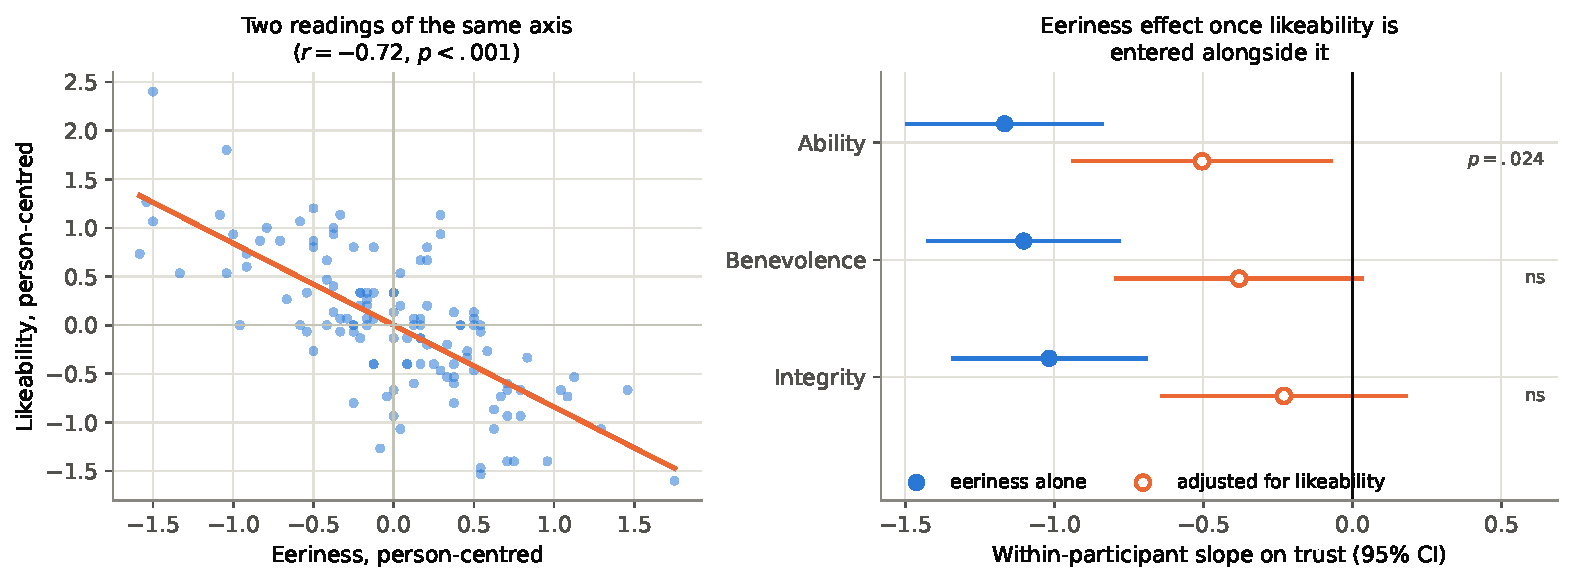
\includegraphics[width=0.74\textwidth]{fig_h3_likeability}
  \end{center}
  \vspace{-0.4em}
  \begin{columns}[T,onlytextwidth]
    \begin{column}{0.32\textwidth}\stat{52\%}{shared variance}{knblue}\end{column}
    \begin{column}{0.32\textwidth}\stat{$-0.50$}{eeriness on ability, joint model}{knred}\end{column}
    \begin{column}{0.32\textwidth}\stat{3 of 3}{trust subscales where likeability holds}{kngreen}\end{column}
  \end{columns}
  \vspace{0.3em}
  {\centering\scriptsize\color{kngrey}Joint model: eeriness holds on ability ($p=.024$), drops out on benevolence ($p=.075$) and integrity ($p=.273$).\par}
\end{frame}

\begin{frame}{Backup — Why a ranking, and how it was read}
  \keymsg{A ranking of all three, because a single choice would all go to the real speaker.}
  \begin{columns}[T,onlytextwidth]
    \begin{column}{0.55\textwidth}
      \panelheadsm{Why rank, not pick one}
      \pts{%
        \item C1 was expected to win, so a single pick would \hl{pile onto C1}
        \item Then nothing would be left to separate \hl{C2 from C3}
        \item Adapted from the single-choice task of Canales~[7]}
      \vspace{0.3em}
      \panelheadsm{What it measures}
      \pts{%
        \item Ratings: what people \hl{believe} about the advisor
        \item \emph{Most want to consult}: whether they would \hl{act} on it, the primary behavioural measure}
    \end{column}
    \begin{column}{0.42\textwidth}
      \stat{3}{rankings: consult, trustworthy, unsettling}{knblue}\\[0.4em]
      \stat{Friedman}{then Holm-corrected Wilcoxon on the three pairs. Ranks are ordinal}{knblue}\\[0.4em]
      \noindent\colorbox{knlight}{\parbox{\dimexpr\linewidth-2\fboxsep\relax}{\vspace{3pt}\scriptsize\raggedright
        \bad{Unsettling:} the question read \emph{most to least}, but the columns said 1 (Best) to 3 (Worst). Null either way, $p=.60$.\vspace{3pt}}}
    \end{column}
  \end{columns}
\end{frame}

\begin{frame}{Backup — Full statistics table}
  \keymsg{The real speaker differs from both avatars on every subscale. The avatars differ on none.}
  {\centering\footnotesize\setlength{\tabcolsep}{5pt}\renewcommand{\arraystretch}{1.2}
  \begin{tabular}{@{}lllll@{}}
    \toprule
    \textbf{Subscale} & \textbf{Omnibus} & \textbf{C1 vs C2} & \textbf{C1 vs C3} & \textbf{C2 vs C3} \\
    \midrule
    Likeability  & $F(2,80)=26.85$, $\eta^2_p=.40$ & $g=0.92$ & $g=1.02$ & \bad{$p=.54$, $g=0.08$} \\
    Eeriness     & $F(2,80)=20.39$, $\eta^2_p=.34$ & $g=0.98$ & $g=0.98$ & \bad{$p=.66$, $g=0.07$} \\
    Ability      & $F(2,80)=10.91$, $\eta^2_p=.21$ & $g=0.53$ & $g=0.75$ & \bad{$p=.21$, $g=0.20$} \\
    Benevolence  & $F(2,80)=14.31$, $\eta^2_p=.26$ & $g=0.59$ & $g=0.79$ & \bad{$p=.18$, $g=0.19$} \\
    Integrity    & $F(2,80)=12.47$, $\eta^2_p=.24$ & $g=0.66$ & $g=0.80$ & \bad{$p=.27$, $g=0.16$} \\
    \bottomrule
  \end{tabular}\par}
  {\centering\tiny\color{kngrey}All omnibus $p<.001$. All C1 comparisons significant: $p=.004$ and $p=.001$ on C1 vs C2 ability and integrity, otherwise $p<.001$.\par}
  \vspace{0.5em}
  \begin{columns}[T,onlytextwidth]
    \begin{column}{0.49\textwidth}
      \panelheadsm{Order checks}
      \pts{%
        \item Video position: \good{no effect} on any subscale
        \item Study version: likeability ($p=.002$) and eeriness ($p=.008$), \good{no trust subscale}}
    \end{column}
    \begin{column}{0.49\textwidth}
      \panelheadsm{H3 models}
      \pts{%
        \item ICC: eeriness $.48$ to $.57$, likeability $.57$ to $.63$
        \item Half or more of trust variance is \hl{between} people}
    \end{column}
  \end{columns}
\end{frame}

\begin{frame}{Backup — The mismatch evidence}
  \keymsg{Eeriness comes from a mismatch between features, not from realism itself.}
  \begin{columns}[T,onlytextwidth]
    \begin{column}{0.58\textwidth}
      \panelheadsm{K\"atsyri et al.\ 2015~[17]}
      \pts{%
        \item Review of \hl{17 studies}, testing the competing valley explanations
        \item \emph{More human-like means a dip}: held in only \bad{1 of 8}
        \item \hl{Perceptual mismatch}, features at different realism levels: \good{4 of 4}
        \item One study: a \hl{mismatched face and voice} was rated eerier}
      \vspace{0.3em}
      \panelheadsm{Cihodaru-\c{S}tefanache \& Podina 2025~[16]}
      \pts{%
        \item Recent review of embodied conversational agents
        \item Reaches the \hl{same conclusion}: mismatch, not realism}
    \end{column}
    \begin{column}{0.39\textwidth}
      \centering
      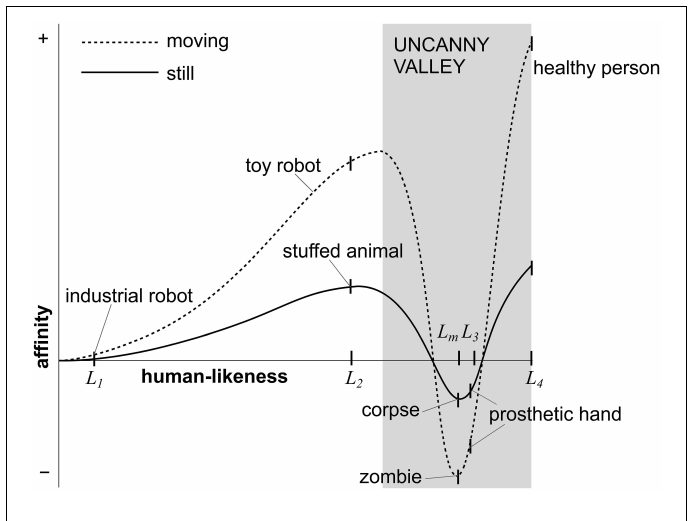
\includegraphics[width=\textwidth]{05-4_katsyri_2015_valley_turning_points}\\[-0.1em]
      {\scriptsize\color{kngrey}K\"atsyri et al.~[17]\par}
      \vspace{0.5em}
      \noindent\colorbox{knlight}{\parbox{\dimexpr\linewidth-2\fboxsep\relax}{\vspace{3pt}\scriptsize\raggedright
        \textbf{\color{knblue}Link to C3:} a human voice and human motion on an abstracted face is exactly such a mismatch.\vspace{3pt}}}
    \end{column}
  \end{columns}
\end{frame}

\begin{frame}{Backup — Design compared with Zibrek}
  \keymsg{Same manipulation as Zibrek \& McDonnell~[18], but on a flat screen instead of in VR.}
  \begin{columns}[T,onlytextwidth]
    \begin{column}{0.58\textwidth}
      \centering
      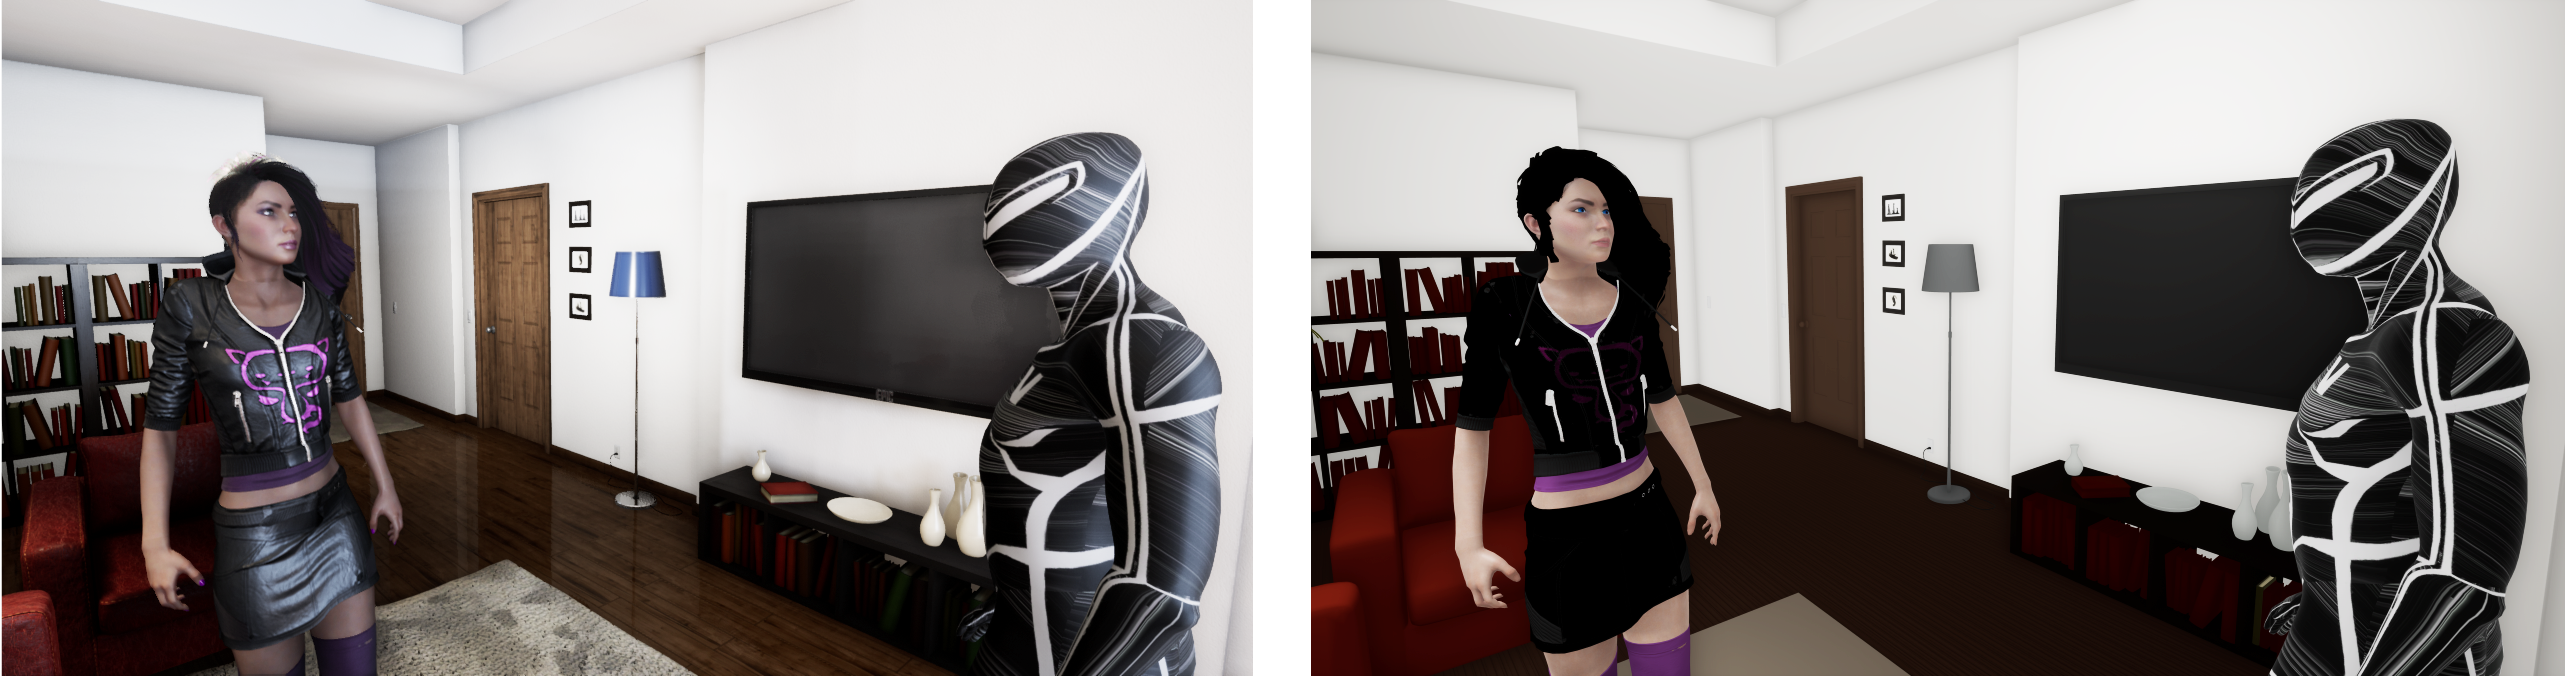
\includegraphics[width=\textwidth]{B-zibrek_2019_render_styles}\\[-0.1em]
      {\scriptsize\color{kngrey}Zibrek \& McDonnell~[18]: realistic and simple\par}
      \vspace{0.4em}
      \begin{columns}[T,onlytextwidth]
        \begin{column}{0.48\textwidth}
          \panelheadsm{Same}
          \pts{%
            \item Only render style changes
            \item One recorded performance
            \item Self-report plus behaviour}
        \end{column}
        \begin{column}{0.48\textwidth}
          \panelheadsm{Different}
          \pts{%
            \item VR body vs \hl{flat video}
            \item Room stylised too
            \item Presence, not trust}
        \end{column}
      \end{columns}
    \end{column}
    \begin{column}{0.40\textwidth}
      \centering
      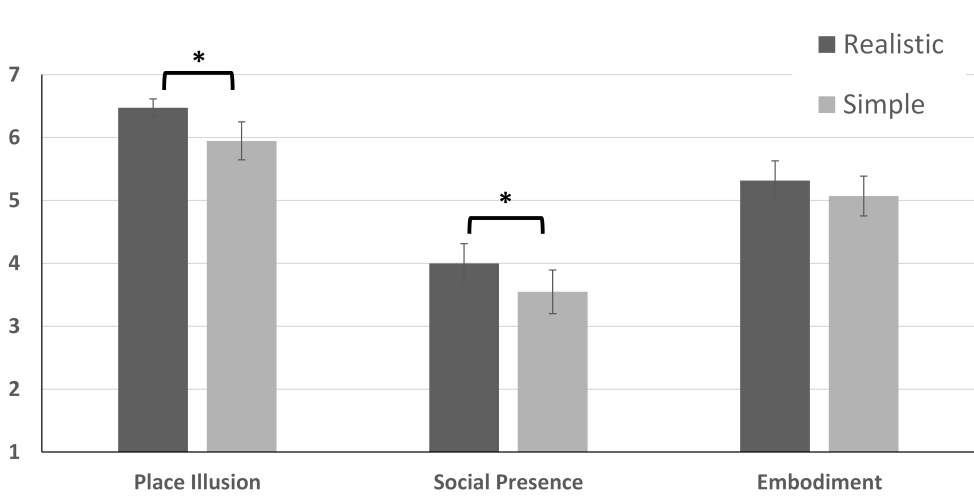
\includegraphics[width=\textwidth]{B-zibrek_2019_results}\\[-0.1em]
      {\scriptsize\color{kngrey}Their result~[18]\par}
      \vspace{0.4em}
      \stat{$d=0.56$}{realism raised social presence. Behaviour did not change}{knblue}\\[0.3em]
      {\centering\scriptsize\color{kngrey}$n=19$ in VR, against $n=41$ here\par}
    \end{column}
  \end{columns}
\end{frame}

\begin{frame}{Backup — Counterbalancing options}
  \keymsg{Three versions was what 41 participants allowed.}
  \begin{columns}[T,onlytextwidth]
    \begin{column}{0.32\textwidth}\stat{3}{versions, Latin square, about 14 people each. \textbf{Used}}{knblue}\end{column}
    \begin{column}{0.32\textwidth}\stat{6}{versions, all condition orders, about 7 people each}{kngrey}\end{column}
    \begin{column}{0.32\textwidth}\stat{36}{versions, every condition and scenario order ($3!\times3!$), about 1 each}{kngrey}\end{column}
  \end{columns}
  \vspace{0.8em}
  \pts{%
    \item The Latin square puts each condition \hl{once in each position}
    \item Scenario order was held fixed, so only the conditions rotated
    \item Six versions would need about \hl{twice the sample}
    \item \bad{Cost:} carryover between specific pairs, such as C1 $\to$ C3, cannot be estimated}
\end{frame}

\begin{frame}{Backup — Which version differed, and on what}
  \keymsg{The groups differed on eeriness and likeability, not on trust.}
  \begin{columns}[T,onlytextwidth]
    \begin{column}{0.42\textwidth}
      {\centering\small\setlength{\tabcolsep}{5pt}\renewcommand{\arraystretch}{1.3}
      \begin{tabular}{@{}llccc@{}}
        \toprule
        \textbf{C1 sat} & \textbf{Ver.} & \textbf{n} & \textbf{Eerie} & \textbf{Liked} \\
        \midrule
        1st & C & 14 & \bad{3.01} & \bad{2.91} \\
        2nd & A & 15 & 2.76 & 3.33 \\
        3rd & B & 12 & \good{2.32} & \good{4.04} \\
        \bottomrule
      \end{tabular}\par}
      \vspace{0.5em}
      \pts{%
        \item Likeability $p=.002$, eeriness $p=.008$
        \item Trust: \good{all null}, $p=.14$ to $.30$}
    \end{column}
    \begin{column}{0.55\textwidth}
      \pts{%
        \item The \hl{later the real speaker} came, the milder the ratings
        \item Versions B and C carry it: $g=1.50$ likeability, $g=-1.11$ eeriness
        \item Fits an \hl{anchoring} effect: a real human first makes what follows look worse
        \item \good{H1 survives:} C2 minus C3 eeriness does not follow it, $p=.244$
        \item \bad{Cannot rule out:} a version is a group \emph{and} an order}
    \end{column}
  \end{columns}
  \vfill
  {\tiny\color{kngrey}Supplementary analysis, not in the thesis. Likeability's C2 minus C3 contrast does vary, $F=3.43$, $p=.043$, uncorrected.\par}
\end{frame}

\begin{frame}{Backup — Which condition moved}
  \keymsg{Both avatars moved together, so the contrast H1 tests was preserved.}
  \begin{columns}[T,onlytextwidth]
    \begin{column}{0.32\textwidth}
      \panelheadsm{Eeriness, 1--5}
      {\centering\scriptsize\setlength{\tabcolsep}{3.5pt}\renewcommand{\arraystretch}{1.2}
      \begin{tabular}{@{}lccc@{}}
        \toprule
        \textbf{C1 sat} & \textbf{C1} & \textbf{C2} & \textbf{C3} \\
        \midrule
        1st (C) & 2.47 & \bad{3.37} & 3.18 \\
        2nd (A) & 2.12 & 2.92 & 3.23 \\
        3rd (B) & 2.01 & \good{2.46} & \good{2.48} \\
        \midrule
        $p$ & .24 & \bad{.005} & \bad{.039} \\
        \bottomrule
      \end{tabular}\par}
      \pts{\item C1 \good{holds still}\item Both avatars move \hl{together}}
    \end{column}
    \begin{column}{0.32\textwidth}
      \panelheadsm{Likeability, 1--5}
      {\centering\scriptsize\setlength{\tabcolsep}{3.5pt}\renewcommand{\arraystretch}{1.2}
      \begin{tabular}{@{}lccc@{}}
        \toprule
        \textbf{C1 sat} & \textbf{C1} & \textbf{C2} & \textbf{C3} \\
        \midrule
        1st (C) & 3.61 & \bad{2.36} & 2.77 \\
        2nd (A) & 4.04 & 3.23 & 2.73 \\
        3rd (B) & \good{4.53} & \good{3.90} & \good{3.70} \\
        \midrule
        $p$ & \bad{.009} & \bad{.001} & .050 \\
        \bottomrule
      \end{tabular}\par}
      \pts{\item Even C1 shifts\item Strongest on \hl{C2}}
    \end{column}
    \begin{column}{0.32\textwidth}
      \panelheadsm{Trust composite, 1--7}
      {\centering\scriptsize\setlength{\tabcolsep}{3.5pt}\renewcommand{\arraystretch}{1.2}
      \begin{tabular}{@{}lccc@{}}
        \toprule
        \textbf{C1 sat} & \textbf{C1} & \textbf{C2} & \textbf{C3} \\
        \midrule
        1st (C) & 4.94 & 3.48 & 3.75 \\
        2nd (A) & 5.28 & 4.73 & 3.73 \\
        3rd (B) & 5.64 & 4.70 & 4.50 \\
        \midrule
        $p$ & .46 & .08 & .45 \\
        \bottomrule
      \end{tabular}\par}
      \pts{\item \good{Nothing significant}\item H2 to H4 untouched}
    \end{column}
  \end{columns}
  \vfill
  {\tiny\color{kngrey}C2 minus C3 eeriness by version: $-0.31$, $-0.02$, $+0.19$, $F(2,38)=1.46$, $p=.244$. Likeability contrast varies ($p=.043$), trust contrast does not ($p=.091$). Supplementary analysis, not in the thesis.\par}
\end{frame}

\end{document}
